\chapter{Streszczenie w języku polskim i angielskim}
\label{cha:Lab001}
\makeatletter

W danym projekcie zrealizowany został system zarządzania biblioteką. Wszystkie dane są pobierane z bazy, co umożliwia mobilność programu dla użytkowników. System pozwala na łatwe założenie konta czytelnika. Wyszukiwarka umożliwia znalezienie książek po tytule, autorze i kategorii. Wypożyczeń można dokonywać z poziomu konta czytelnika, gdzie wyświetlane są również ewentualne zaległości. Zwrotu książek dokonuje konto bibliotekarza. Bibliotekarz ma możliwość dodawania, edytowania i usuwania książek z bazy. Może także przeglądać wypożyczenia czytelników oraz oznaczać książki jako zwrócone. System pozwala bibliotekarzowi na eksportowanie i importowanie danych (użytkownicy, wypożyczenia, książki).\bigskip

In a given project, a library management system is realized. All data is extracted from the database, which allows mobility of the program for users. Also, it allows easy creation of a reader's account. Search allows finding books by title, author, and category. Borrowing can be done via the reader's account, and backlogs are displayed. Returning books is done through the librarian's account. The librarian can add, edit, and delete books. Also, they can see the readers' loans and mark a book as returned. The librarian can export and import data (users, loans, books).


\chapter{Wprowadzenie i analiza problemu}
Celem tego projektu jest efektywne zarządzanie danymi biblioteki. Aplikacja umożliwia łatwe przeglądanie, edytowanie oraz dodawanie danych do bazy. Dzięki intuicyjnemu interfejsowi użytkownik nie musi posiadać zaawansowanej wiedzy na temat systemów zarządzania bazami danych. Obecnie baza działa lokalnie, jednak architektura pozwala na wdrożenie jej na serwer online. 

\noindent \textbf{Wymagania funkcjonalne}
\begin{itemize}
    \item Umożliwia zakładanie kont czytelników i logowanie do systemu (z uwzględnieniem ról).
    \item Pozwala na wyszukiwanie książek według tytułu, autora i kategorii.
    \item Pozwala wyszukiwać użytkowników według imienia, nazwiska, nazwy użytkownika i roli.
    \item Użytkownicy mogą wypożyczać książki, a system śledzi zaległości i ewentualne kary. 
    \item Bibliotekarz ma możliwość dodawania, edytowania i usuwania książek. 
    \item System umożliwia zwrot książek poprzez konto bibliotekarza.
    \item Eksportowanie i importowanie danych do bazy biblioteki poprzez konto bibliotekarza.
    \item Zmiana hasła.
\end{itemize}

\noindent \textbf{Wymagania niefunkcjonalne}
\begin{itemize}
    \item System powinien zapewniać wysoką wydajność w przetwarzaniu zapytań do bazy danych.     
    \item Interfejs użytkownika (GUI) powinien być intuicyjny, estetyczny i łatwy w obsłudze.
    \item System powinien być skalowalny i bezpieczny, aby obsłużyć rosnącą liczbę użytkowników.
\end{itemize}

\noindent \textbf{Analiza rozwiązań o podobnym przeznaczeniu}
\bigskip
W celu zdefiniowania wymagań funkcjonalnych systemu, przeanalizowano trzy popularne rozwiązania biblioteczne:
\begin{itemize}
    \item Koha (Open-Source) \cite{Koha} – globalny system webowy. Oferuje pełną obsługę cyklu wypożyczeń, automatyczną kontrolę stanów magazynowych oraz automatyczne naliczanie kar za przetrzymanie książek. Opiera się na skomplikowanych formatach bibliotecznych (MARC21).
    \item MAK+ (MakPlus) \cite{MAK+} – polski system chmurowy Instytutu Książki. Wdraża system ról (bibliotekarz/czytelnik) oraz automatyczne blokady kont dla dłużników. Umożliwia pobieranie danych o książkach bezpośrednio z bazy centralnej po kodzie ISBN.
    \item MOL NET+ \cite{MOLNET+} – komercyjny system chmurowy, standard w polskich szkołach. Posiada intuicyjny panel administratora, automatyczną integrację z e-dziennikami oraz moduły do zarządzania kopiami zapasowymi.
\end{itemize}


\chapter{Wymagania systemowe} \label{sec:wymagania}
Aplikacja została zaprojektowana na platformę .NET. Minimalne wymagania do uruchomienia to:
\begin{itemize}
    \item Procesor: Intel i3 / AMD Ryzen 3. 
    \item Pamięć RAM: Minimum 4 GB.
    \item System operacyjny: Windows 10/11.
    \item .NET Desktop Runtime (kompatybilny z wersją użytą w projekcie).
\end{itemize}

Do otwarcia projektu i jego dalszego rozwoju zalecane jest pobranie środowiska Microsoft Visual Studio (18.5.2) ze strony \url{https://visualstudio.microsoft.com/downloads/}. 
Dodatkowe narzędzie to SQL Server Management Studio 22 (22.5.2) można pobrać na stronie \url{https://learn.microsoft.com/en-us/ssms/install/install}.


\chapter{Architektura i struktura aplikacji}
Architektura aplikacji została podzielona na warstwy zgodnie z dobrymi praktykami programowania w C\# (WPF). Wyróżniamy podział na modele, bazę danych, interfejs graficzny i logikę biznesową.

\begin{figure}[H]
    \centering
    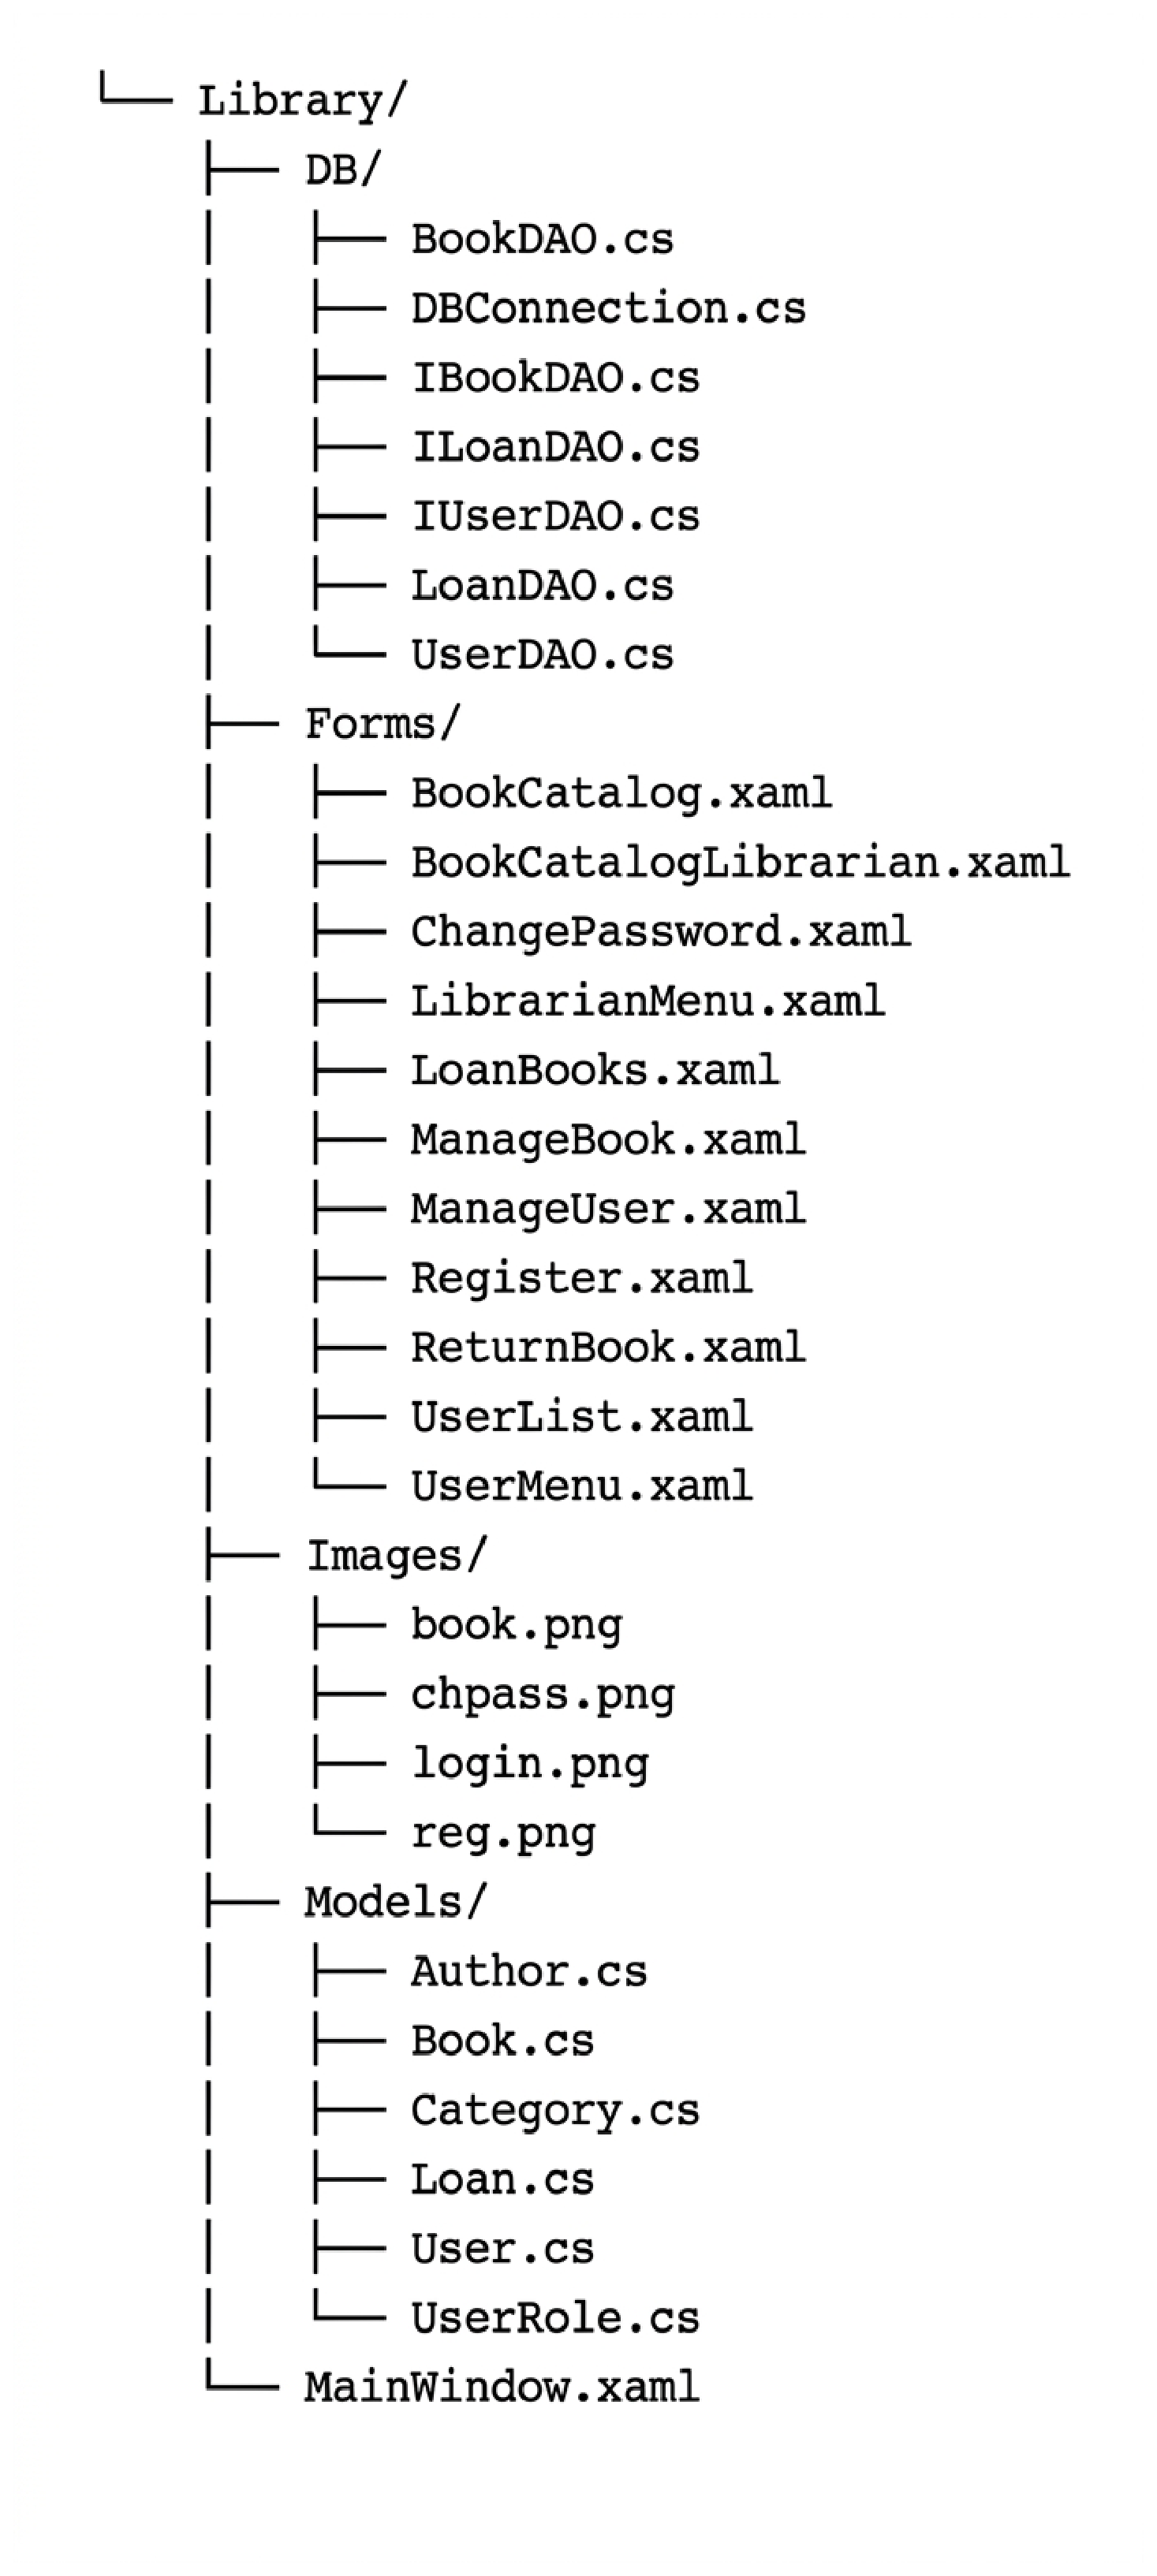
\includegraphics[width=0.4\linewidth]{figures/folders.eps}
    \caption{Struktura folderów.\label{fig:folders}}
\end{figure}

W folderze \texttt{Models} zdefiniowano obiekty (klasy encyjne) reprezentujące 
tabele z bazy danych. Są to: \texttt{User}, \texttt{Loan}, \texttt{Category}, 
\texttt{Book}, \texttt{Author} oraz \texttt{UserRole}. 
Klasy te odzwierciedlają strukturę relacyjną; zawierają właściwości 
odpowiadające kolumnom w tabelach (np. \texttt{FirstName}, \texttt{LastName}, \texttt{ISBN}) 
oraz właściwości nawigacyjne używane przez Entity Framework do obsługi 
relacji między obiektami (np. kolekcja \texttt{Loans} w klasie \texttt{User}).

\begin{figure}[H]
    \centering
    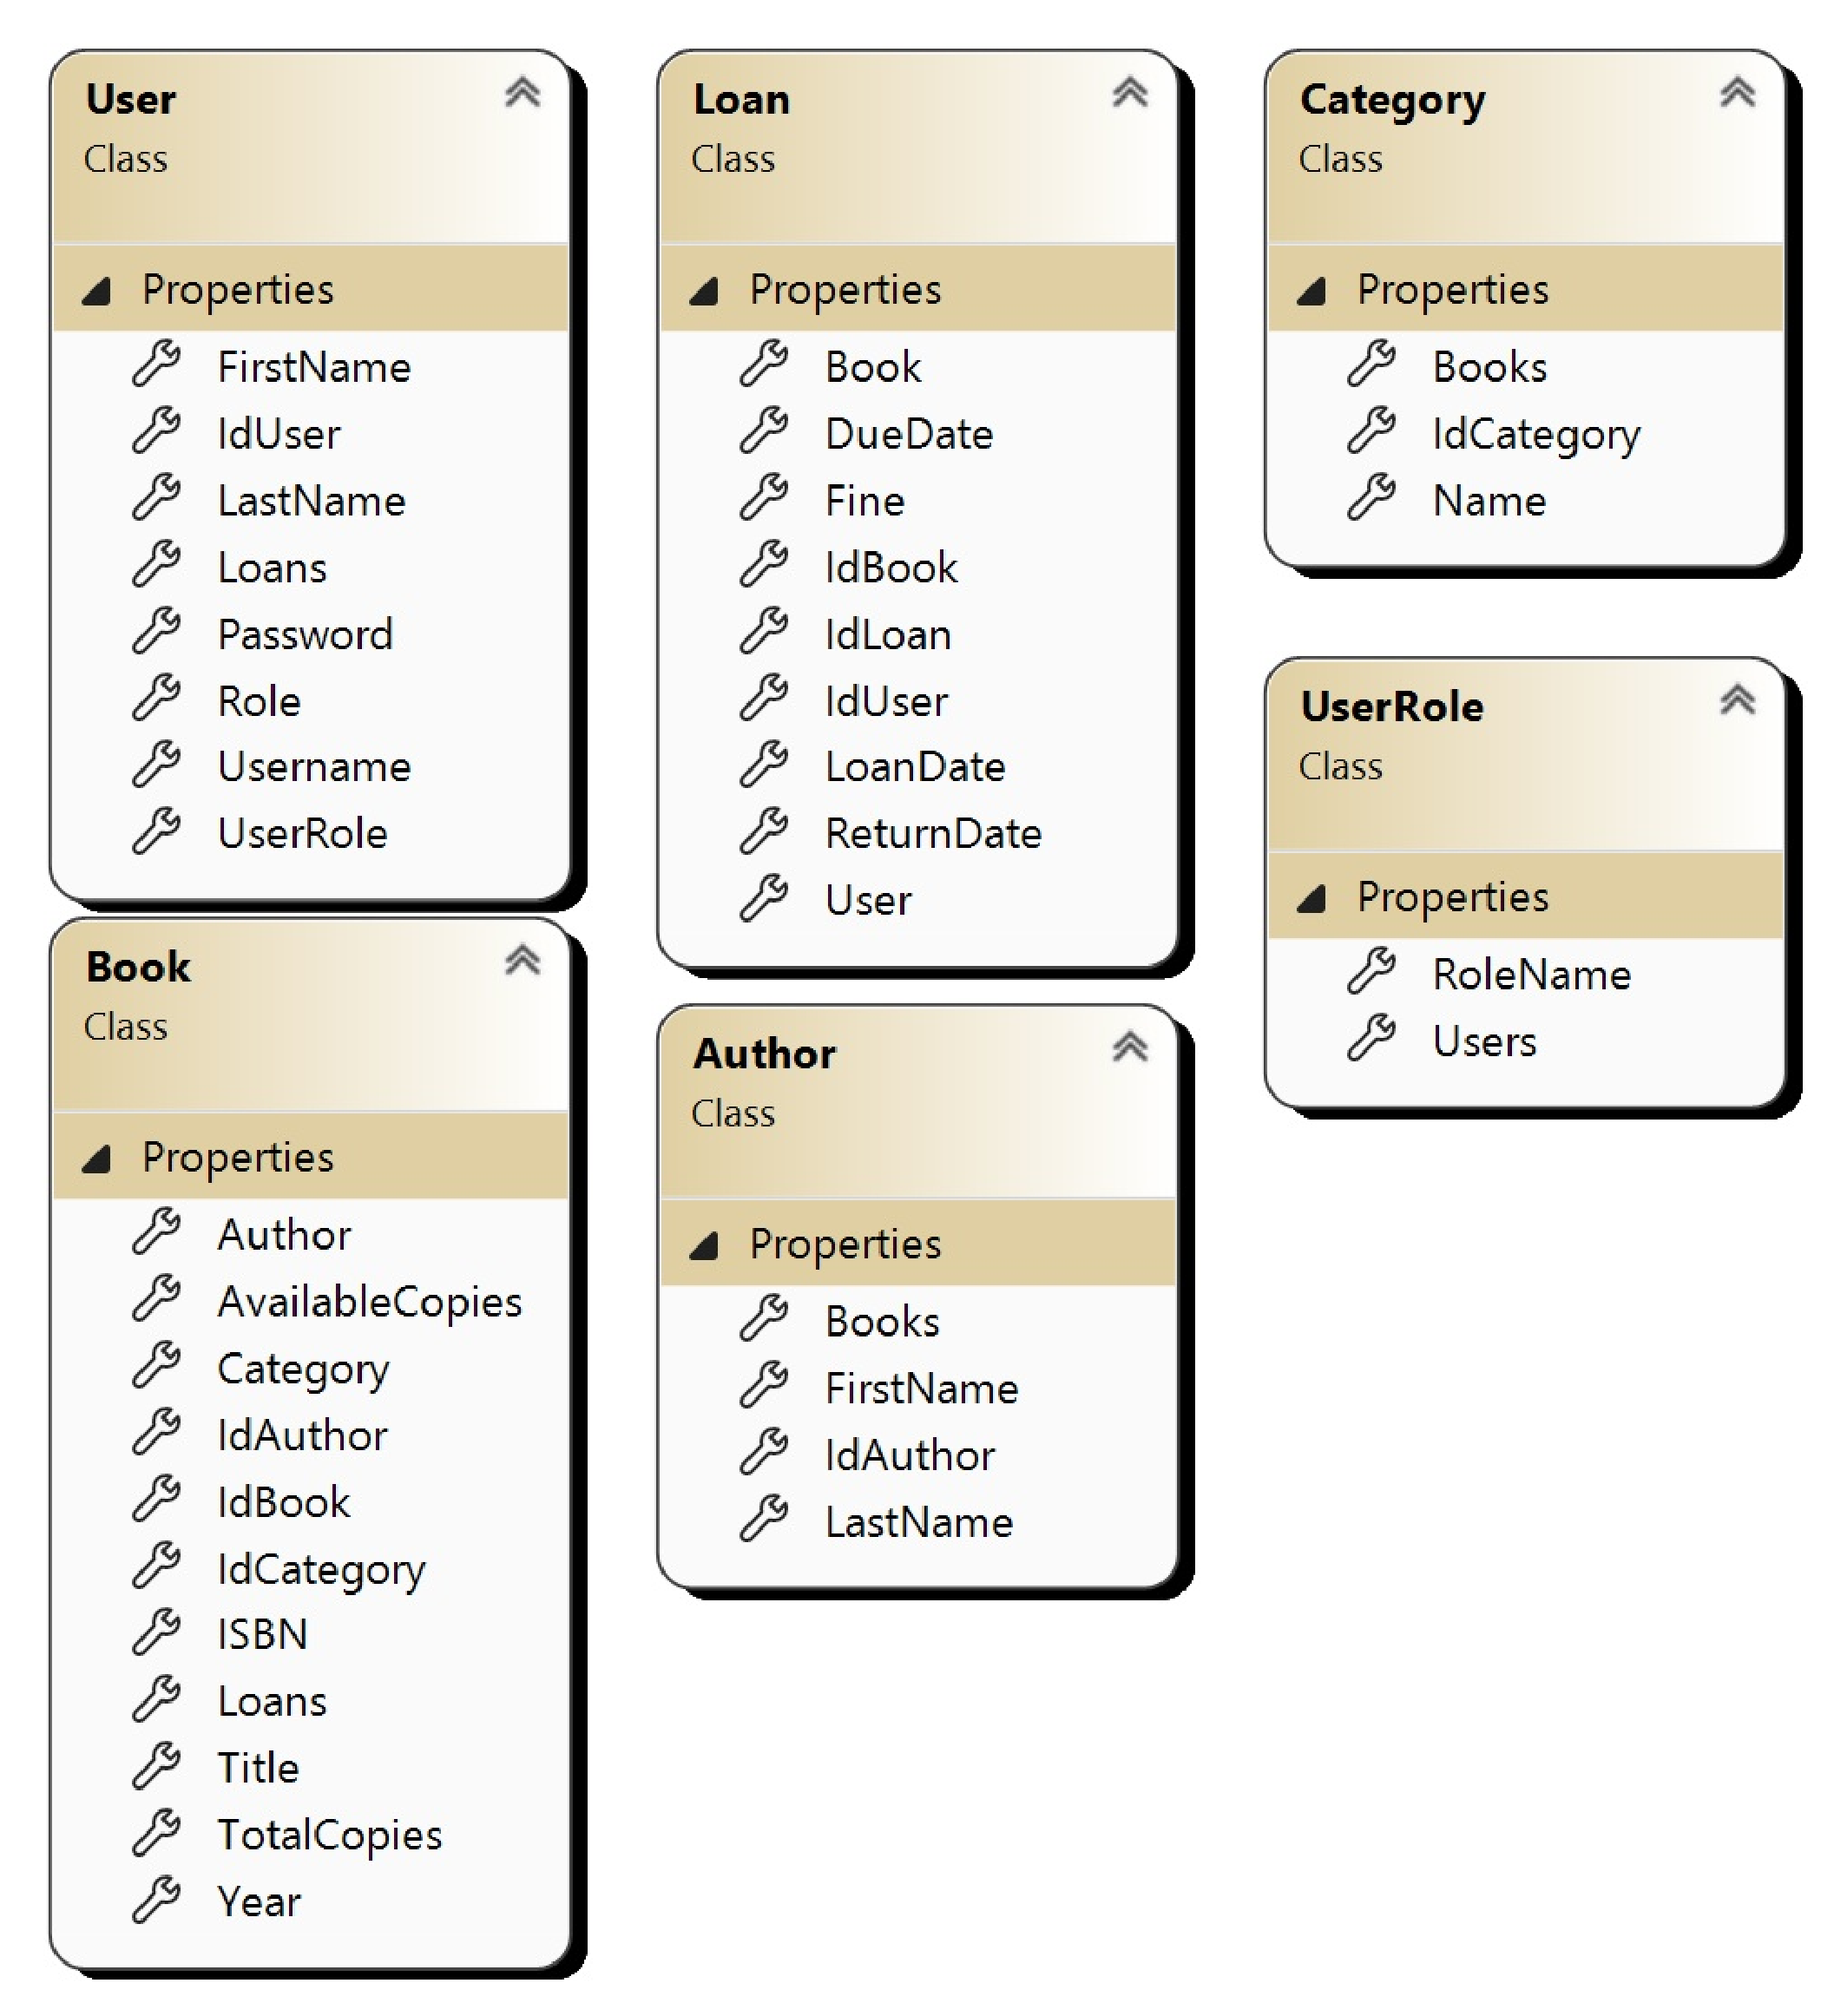
\includegraphics[width=0.8\linewidth]{figures/UML.eps}
    \caption{Diagram klas - modele bazodanowe.\label{fig:uml_models}}
\end{figure}

W folderze \texttt{DB} znajduje się logika dostępu do danych, a \texttt{Forms} zawiera definicje widoków interfejsu. Mechanizmy walidacji wprowadzanych danych i obsługa wyjątków zostały zaimplementowane tak, aby system był stabilny i informował użytkownika o błędach.

\chapter{Technologie wykorzystane w projekcie}
\begin{itemize}
    \item \textbf{C\# (.NET)} \cite{CSharpDocs}: Główny język programowania aplikacji. Został wybrany ze względu na jego silne typowanie, pełne wsparcie dla paradygmatu programowania obiektowego oraz bogaty zbiór wbudowanych bibliotek w środowisku .NET, które znacznie przyspieszają proces tworzenia zaawansowanych i stabilnych aplikacji desktopowych.
    \item \textbf{WPF (Windows Presentation Foundation)} \cite{WPFDocs}: Technologia użyta do zaprojektowania interfejsu użytkownika. Zdecydowano się na WPF ze względu na elastyczność i wyraźne oddzielenie warstwy wizualnej (zapisanej w deklaratywnym języku XAML) od logiki biznesowej w C\#. Dodatkowo WPF posiada zaawansowane mechanizmy wiązania danych (Data Binding), co idealnie współgra z dynamicznym wyświetlaniem informacji z bazy.
    \item \textbf{Microsoft SQL Server} \cite{SQLServerDocs}: Relacyjny system zarządzania bazą danych (RDBMS). Wykorzystano go do trwałego i bezpiecznego przechowywania wszelkich informacji systemowych (użytkownicy, książki, operacje wypożyczeń). Jego wybór podyktowany był bardzo dobrą, natywną integracją z platformą .NET, wysoką wydajnością i świetnymi mechanizmami zabezpieczającymi integralność relacyjną tabel.
    \item \textbf{Entity Framework Core} \cite{EFCoreDocs}: Narzędzie typu ORM (Object-Relational Mapping). Użyto go, aby móc operować na bazie danych bezpośrednio za pomocą bezpiecznie typowanych obiektów w języku C\#, zamiast pisać skomplikowane zapytania SQL w tekście. Usprawniło to proces mapowania struktury bazy na klasy modelu (tzw. encje) oraz przyspieszyło tworzenie operacji CRUD, dodatkowo eliminując ryzyko błędów pokroju SQL Injection.
\end{itemize}

\chapter{Projekt bazy danych}
Baza danych została zaprojektowana z zachowaniem zasad normalizacji i integralności danych, wykorzystując możliwości silnika SQL. Składa się z następujących tabel:

\begin{itemize}
    \item \textbf{user\_role} -- słownik ról systemowych (zawiera wartości \texttt{'reader'} i \texttt{'librarian'}). Posiada jedno pole \texttt{role\_name} pełniące funkcję klucza głównego.
    \item \textbf{Users} -- przechowuje informacje o użytkownikach (bibliotekarzach i czytelnikach). Zawiera unikalną nazwę użytkownika (\texttt{username}), zahashowane hasło (\texttt{password}), imię, nazwisko oraz przypisaną rolę, która jest kluczem obcym powiązanym z tabelą \texttt{user\_role}.
    \item \textbf{Author} -- słownik autorów książek, zawierający imię i nazwisko autora wraz z automatycznie generowanym kluczem \texttt{id\_author} (IDENTITY).
    \item \textbf{Category} -- słownik kategorii literackich, dbający o to, by nazwa każdej kategorii była unikalna (\texttt{UNIQUE}).
    \item \textbf{Book} -- główna tabela przechowująca zasoby biblioteki. Posiada klucze obce do tabel \texttt{Author} oraz \texttt{Category}. Gwarantuje unikalność 13-znakowego numeru \texttt{isbn} oraz dba o integralność liczbową za pomocą ograniczeń \texttt{CHECK} (całkowita i dostępna liczba kopii nie może być mniejsza od zera, a liczba dostępna nie może przekroczyć całkowitej).
    \item \textbf{Loan} -- tabela asocjacyjna realizująca relację wypożyczeń między użytkownikami a książkami. Zapisuje datę wypożyczenia (\texttt{loan\_date}), przewidywany termin zwrotu (\texttt{due\_date}) oraz rzeczywistą datę zwrotu (\texttt{return\_date}). Zawiera także kwotę ewentualnej kary (\texttt{fine}). Zastosowano tutaj mechanizmy kaskadowego usuwania (\texttt{ON DELETE CASCADE}).
\end{itemize}

Aby zapewnić ścisłą kontrolę nad wprowadzanymi danymi, szeroko wykorzystano więzy spójności typu \texttt{CHECK} (np. sprawdzenie poprawności długości numeru ISBN oraz relacji czasowych między datami wypożyczenia a terminem zwrotu) oraz restrykcje kluczy obcych.
\begin{figure}[H]
    \centering
    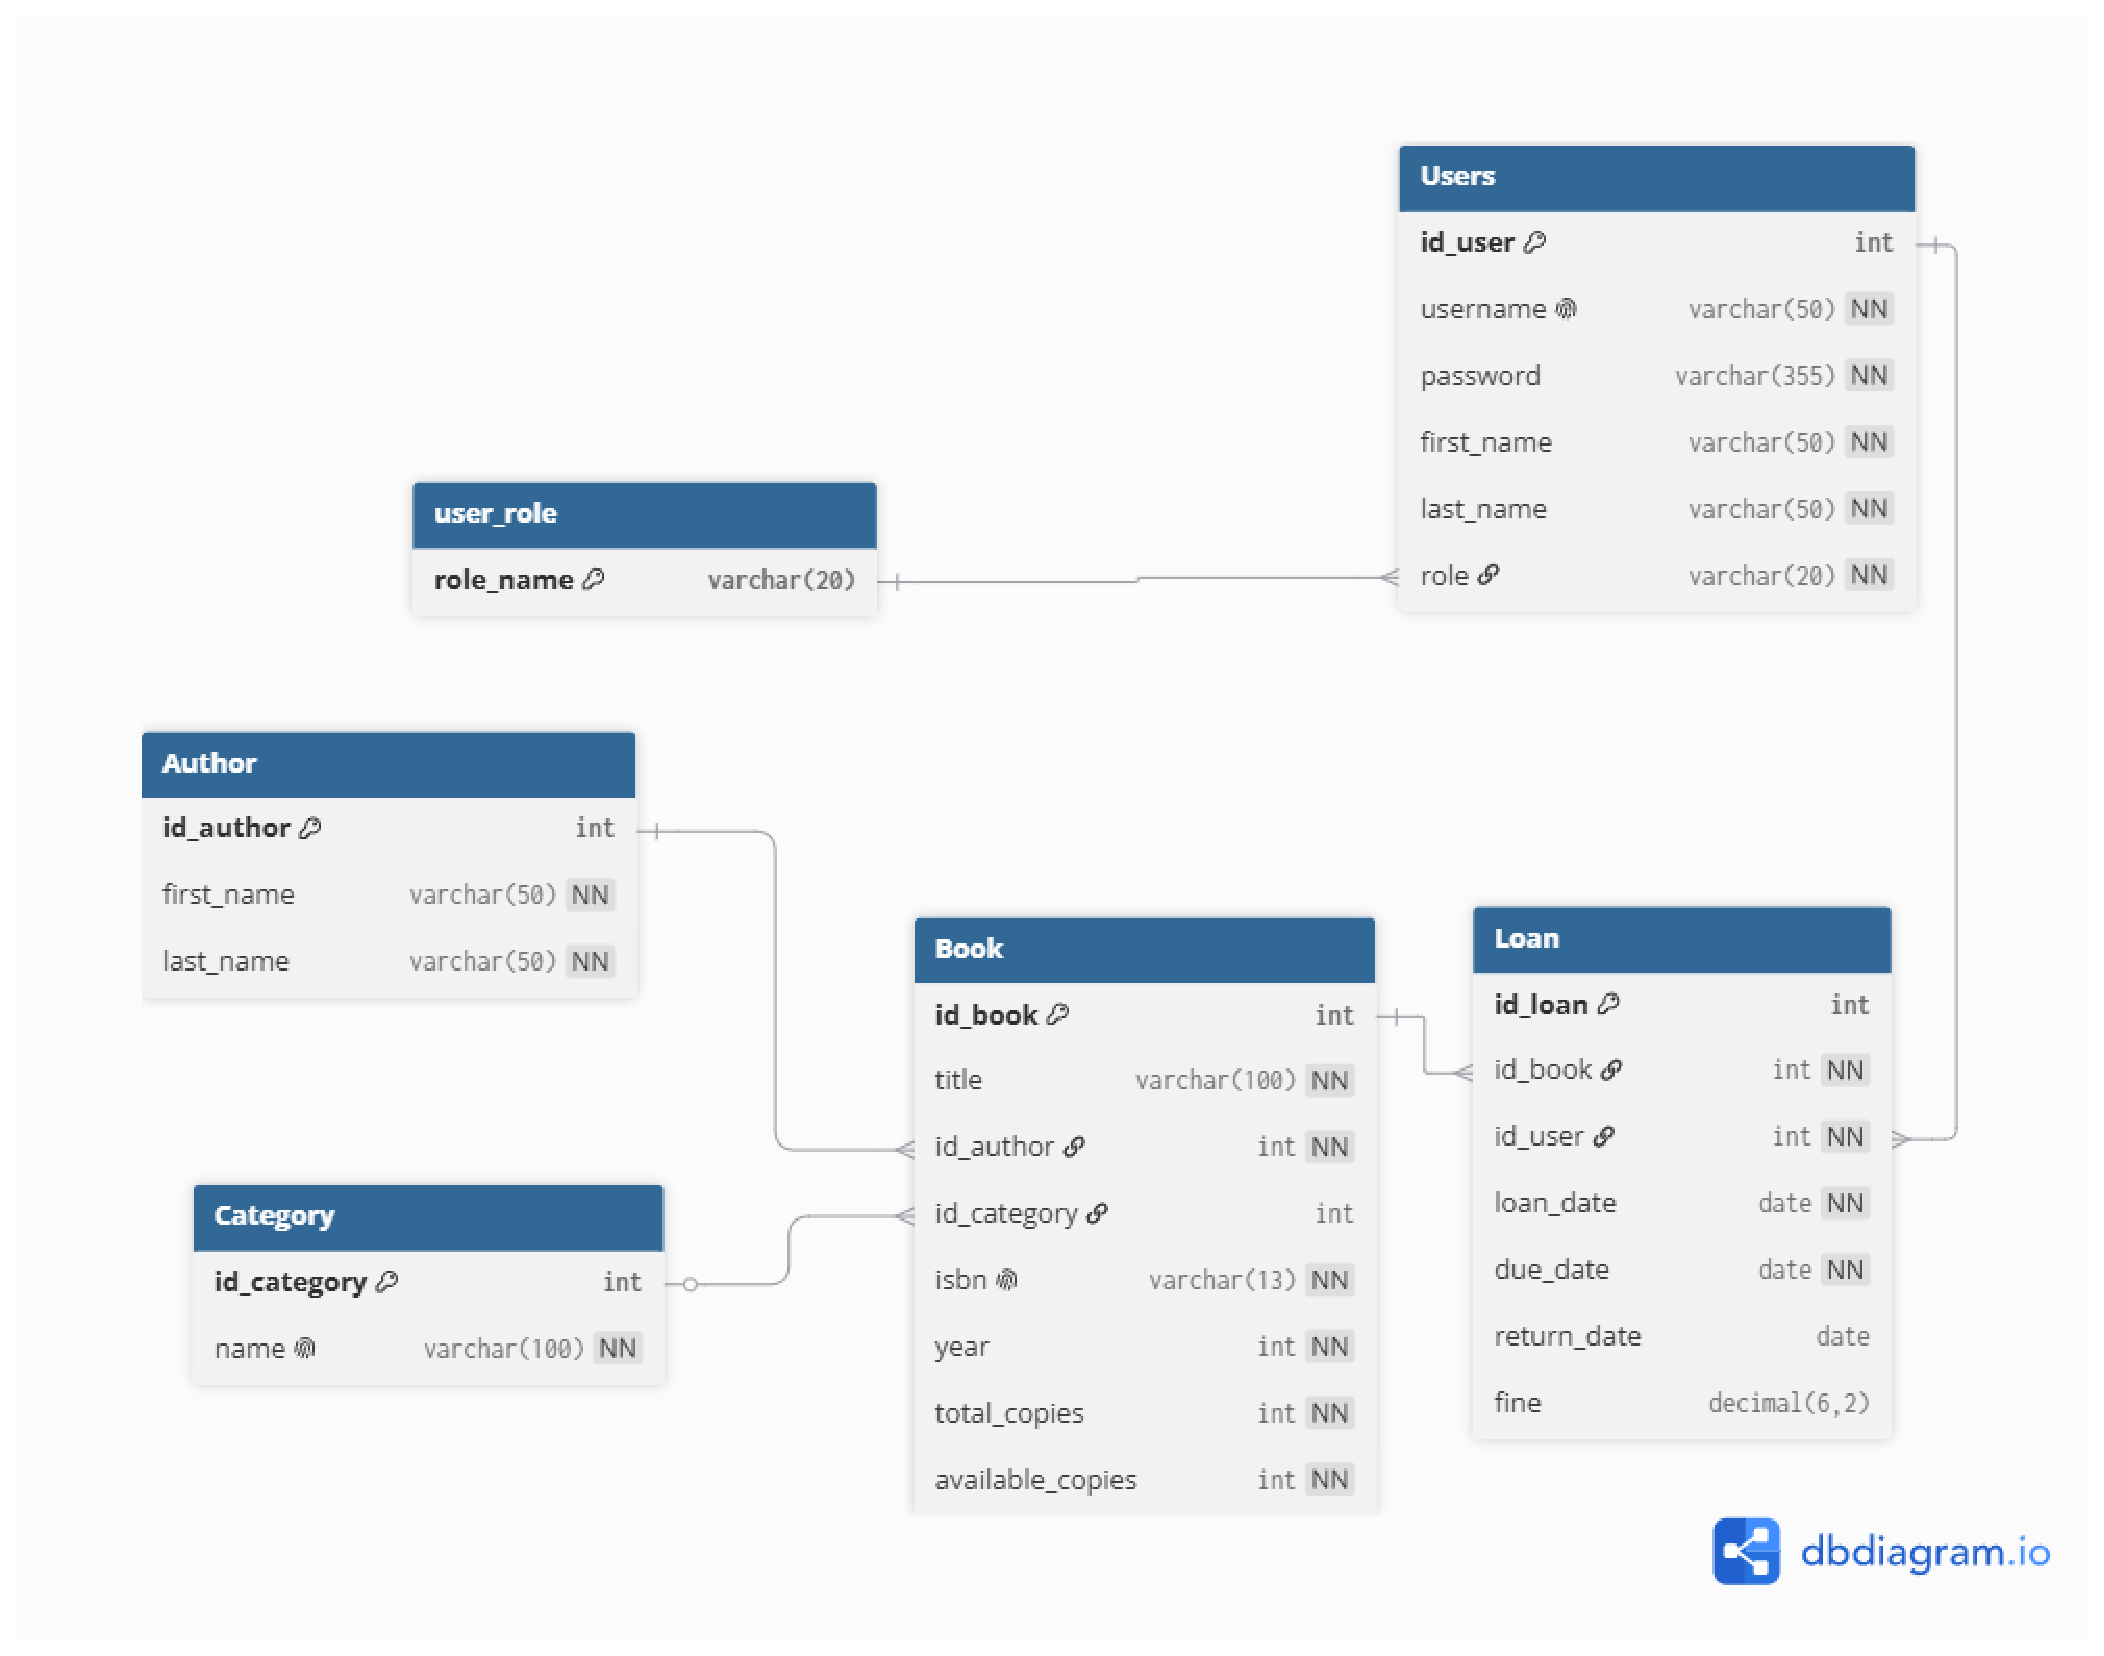
\includegraphics[width=0.8\linewidth]{figures/erd.eps}
    \caption{Diagram ERD projektowanej bazy danych. \cite{DBDiagram} \label{fig:erd}}
\end{figure}


\chapter{Implementacja aplikacji}
Najważniejsze moduły systemu to uwierzytelnianie użytkowników, moduł zarządzania katalogiem książek oraz obsługa procesu wypożyczeń i zwrotów. Interakcje z bazą danych operacje CRUD zostały zrealizowane za pomocą wzorca DAO oraz biblioteki \textbf{Entity Framework Core}. Kod odpowiedzialny za komunikację z bazą zgromadzono w osobnym folderze \texttt{DB}.

Struktura logiki dostępu do danych opiera się na interfejsach: 
\texttt{ILoanDAO}, \texttt{IBookDAO} oraz \texttt{IUserDAO}, 
które definiują kontrakty (metody) niezbędne do obsługi poszczególnych 
encji (np. \texttt{addBook}, \texttt{searchBook}, \texttt{authenticateUser}, 
\texttt{returnLoan}). Klasy \texttt{LoanDAO}, \texttt{BookDAO} i \texttt{UserDAO} 
implementują te interfejsy. Całość komunikacji z silnikiem SQL koordynuje 
klasa \texttt{DBConnection}, dziedzicząca po \texttt{DbContext} z Entity Framework, 
która przechowuje zbiory danych (\texttt{DbSet}) dla każdej encji.

\begin{figure}[H]
    \centering
    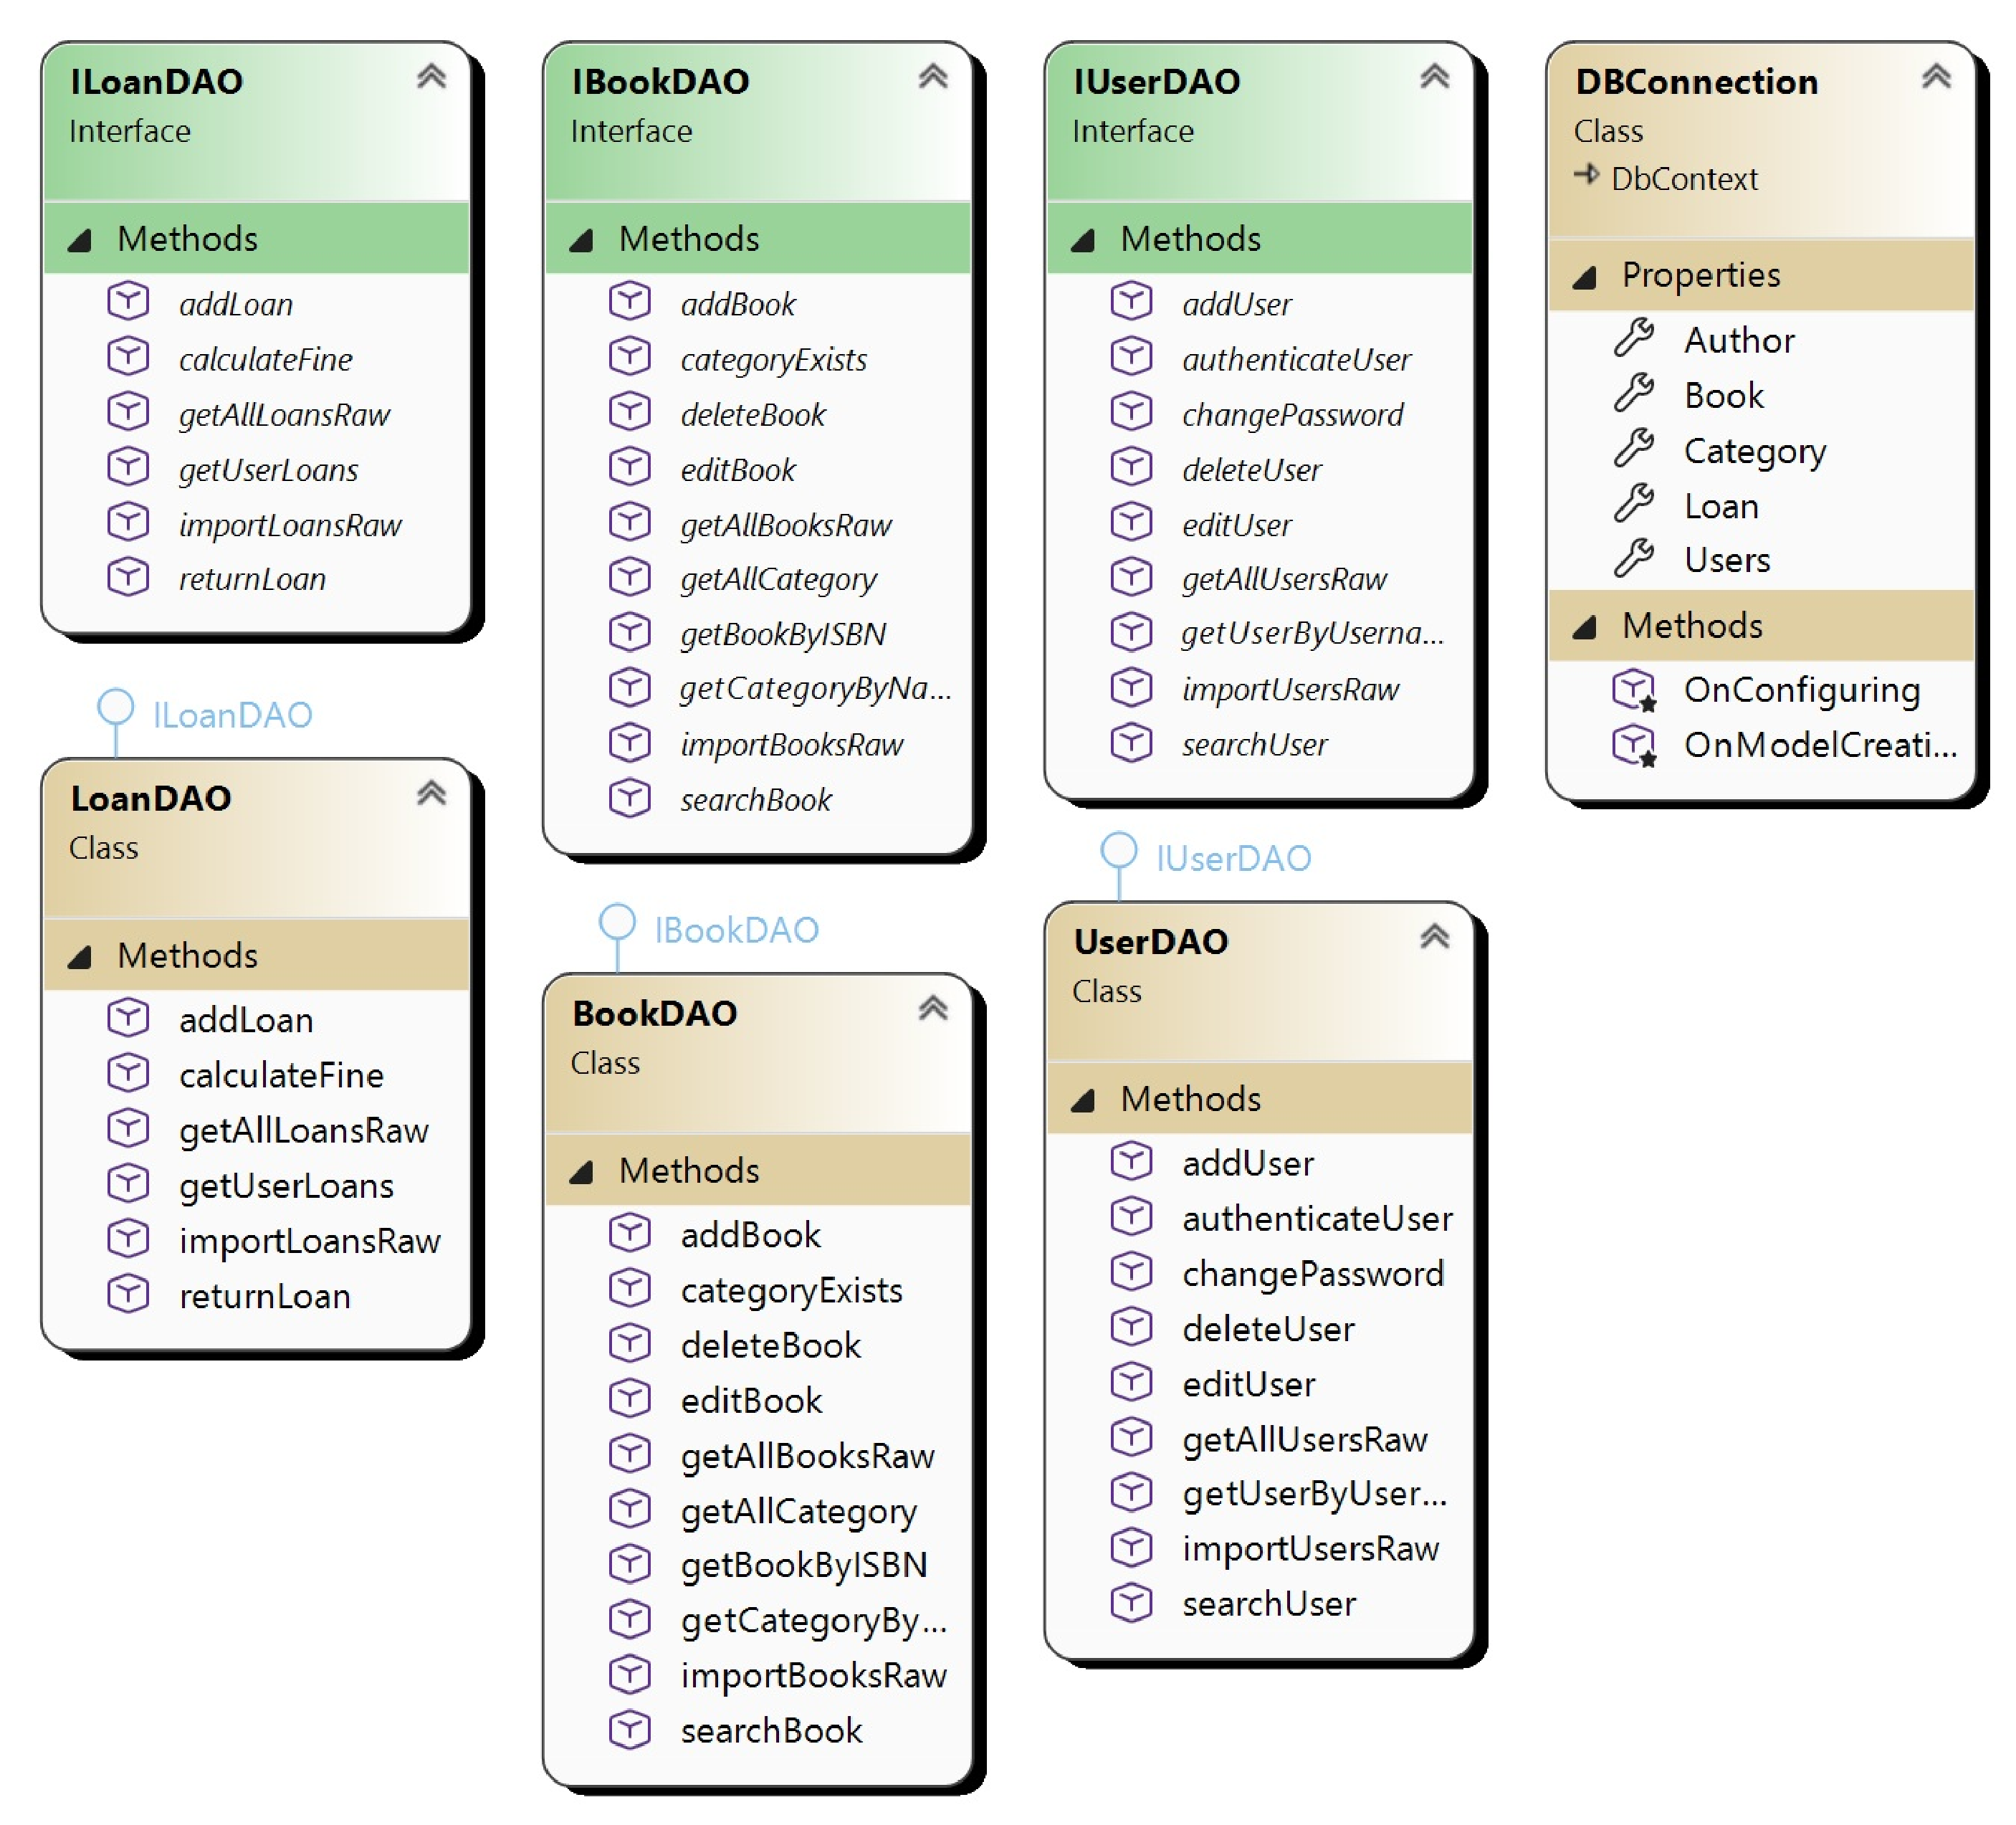
\includegraphics[width=0.9\linewidth]{figures/UML2.eps}
    \caption{Diagram klas - warstwa dostępu do danych (DAO).\label{fig:uml_dao}}
\end{figure}

Do głównych komponentów warstwy dostępu do danych należą:
\begin{itemize}
    \item \textbf{BookDAO} -- obsługuje wyszukiwanie książek, dodawanie, edycję i usuwanie zasobów. Dba również o zarządzanie relacjami. Przy dodawaniu lub edytowaniu książki system automatycznie sprawdza, czy dany autor lub kategoria już istnieją, a jeśli nie, tworzy ich nowe wpisy w bazie.
    \item \textbf{UserDAO} -- realizuje operacje na kontach użytkowników. Umożliwia bezpieczne logowanie i autoryzację z wykorzystaniem hashowania haseł (dzięki mechanizmom \texttt{PasswordHasher}). Ponadto pozwala na rejestrację, edycję, usuwanie profilu oraz zmianę hasła. Zadbano również o to, aby usunięcie użytkownika automatycznie przywracało status dostępności dla niezwróconych przez niego książek.
    \item \textbf{LoanDAO} -- zarządza logiką biznesową wypożyczeń. Zapewnia rezerwację książki (zmniejszenie licznika dostępnych egzemplarzy) i wyznacza termin zwrotu na 14 dni od momentu wypożyczenia. Zwrot książki podnosi licznik z powrotem. Istotnym elementem jest funkcja naliczająca kary (\texttt{calculateFine}), która automatycznie generuje opłatę karną w wysokości 0.50 jednostek za każdy dzień opóźnienia.
\end{itemize}

W systemie zaimplementowano również ważny moduł odpowiedzialny za masowy eksport i import danych (kopie zapasowe). Każda klasa DAO dostarcza metody \texttt{getAll...Raw()}, które pobierają ze struktury pełne kolekcje rekordów do wyeksportowania do pliku. Z kolei metody \texttt{import...Raw()} realizują bezpieczne wprowadzanie danych z powrotem do systemu – usuwają one najpierw istniejące zbiory z bazy, a następnie wprowadzają listę dostarczonych encji, zapewniając synchronizację stanu bazy danych z zaimportowanym plikiem.

Każda operacja wykonywana jest w bezpiecznym bloku klasy zarządzającej połączeniem (\texttt{DBConnection}), gwarantując poprawne otwarcie i zamknięcie sesji bazy danych.

\lstinputlisting[caption= Klasa łącząca się z bazą danych, label=lst:db, style = csStyle]{src/DatabaseConnection.cs}

Na wyższych warstwach aplikacji mechanizmy autoryzacji ograniczają widoczność 
poszczególnych widoków WPF w zależności od roli zalogowanej osoby.

\chapter{Harmonogram realizacji projektu}
Kod źródłowy projektu, historia zmian oraz zarządzanie wersjami odbywało się z 
wykorzystaniem systemu kontroli wersji Git. Repozytorium projektu dostępne 
jest pod adresem: \url{https://github.com/Adoreconfer/Projekt}.

Harmonogram prac nad aplikacją został podzielony na kilka kluczowych 
etapów, których realizacja postępowała w określonych ramach czasowych

\begin{figure}[H]
    \centering
    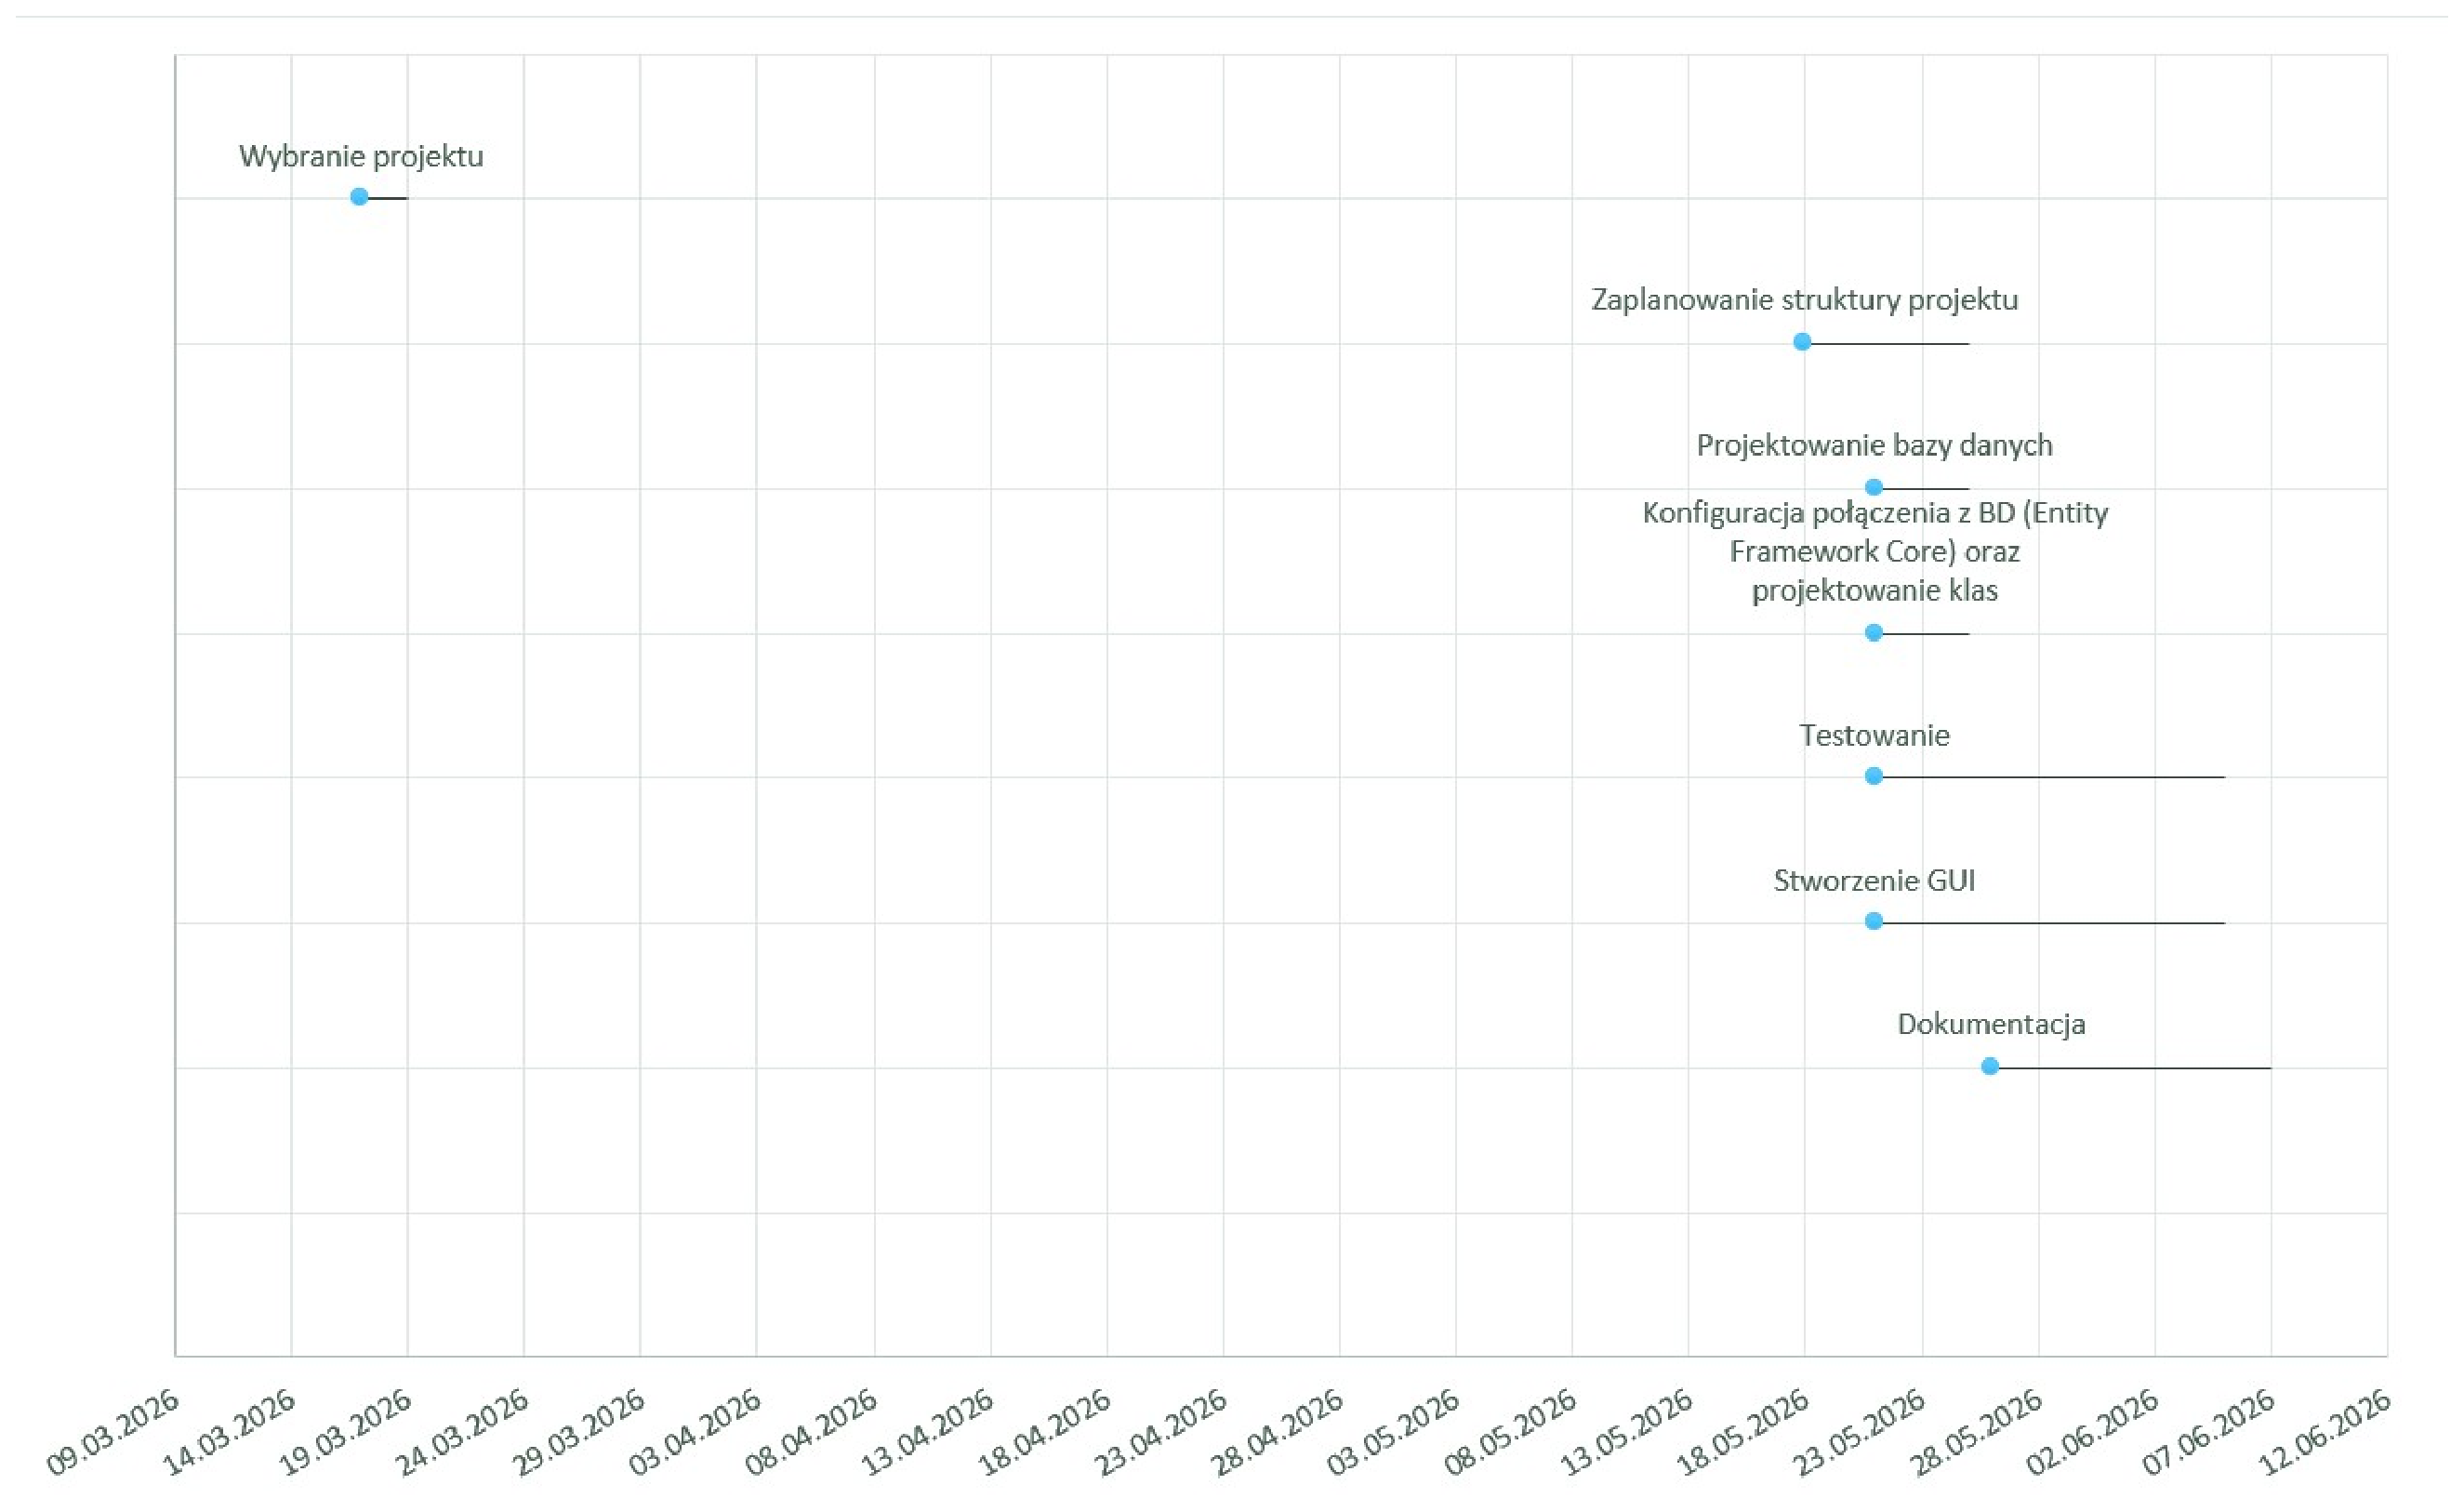
\includegraphics[width=\linewidth]{figures/gantt.eps}
    \caption{Diagram Gantta przedstawiający etapy powstawania aplikacji.\label{fig:gantt}}
\end{figure} 


\chapter{Instrukcja uruchomienia projektu}
Aby poprawnie uruchomić projekt na urządzeniu końcowym, wykonaj następujące kroki:
\begin{enumerate}
    \item Upewnij się, że posiadasz zainstalowane środowisko \textbf{Microsoft Visual Studio} oraz serwer lokalny \textbf{SQL Server}.
    \item Utwórz bazę danych w SQL Server i odtwórz ją korzystając z dostarczonego backup \texttt{LibraryDB.bak}.
    
    \begin{figure}[H]
        \centering
        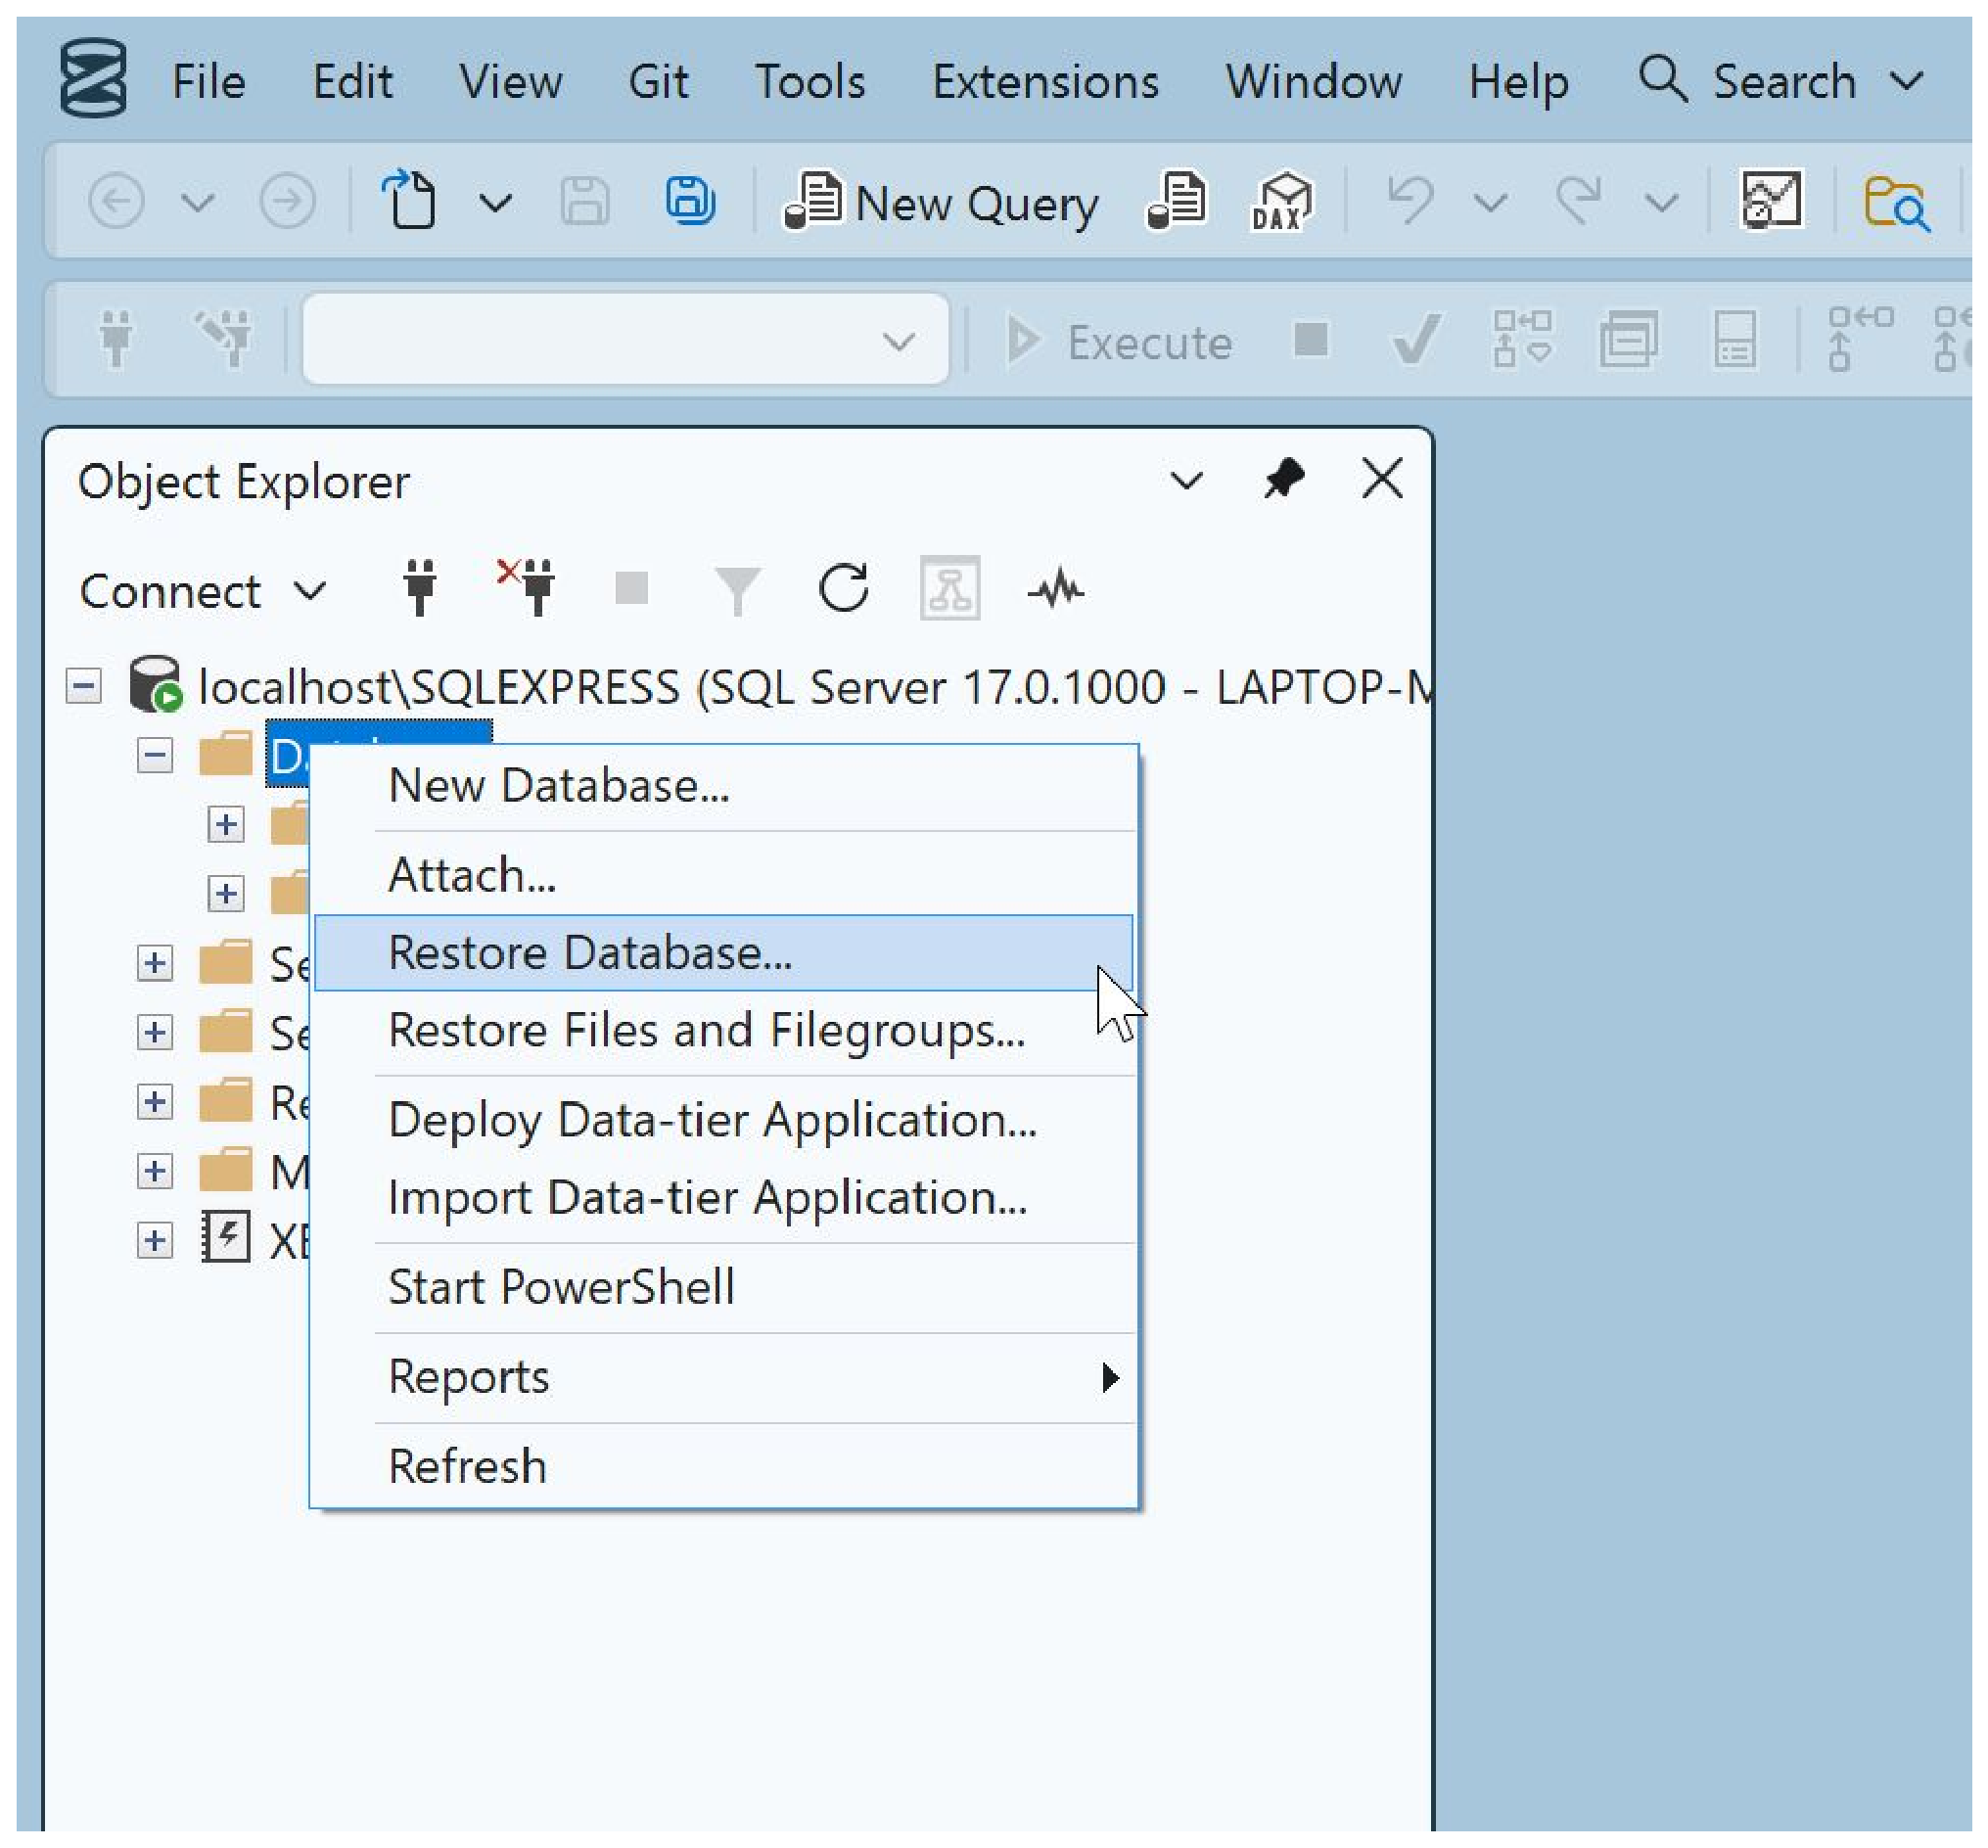
\includegraphics[width=0.5\linewidth]{figures/db1.eps}
        \caption{Przywracanie bazy danych z pliku backupu (cz. 1).\label{fig:db1_setup}}
    \end{figure}
    
    \begin{figure}[H]
        \centering
        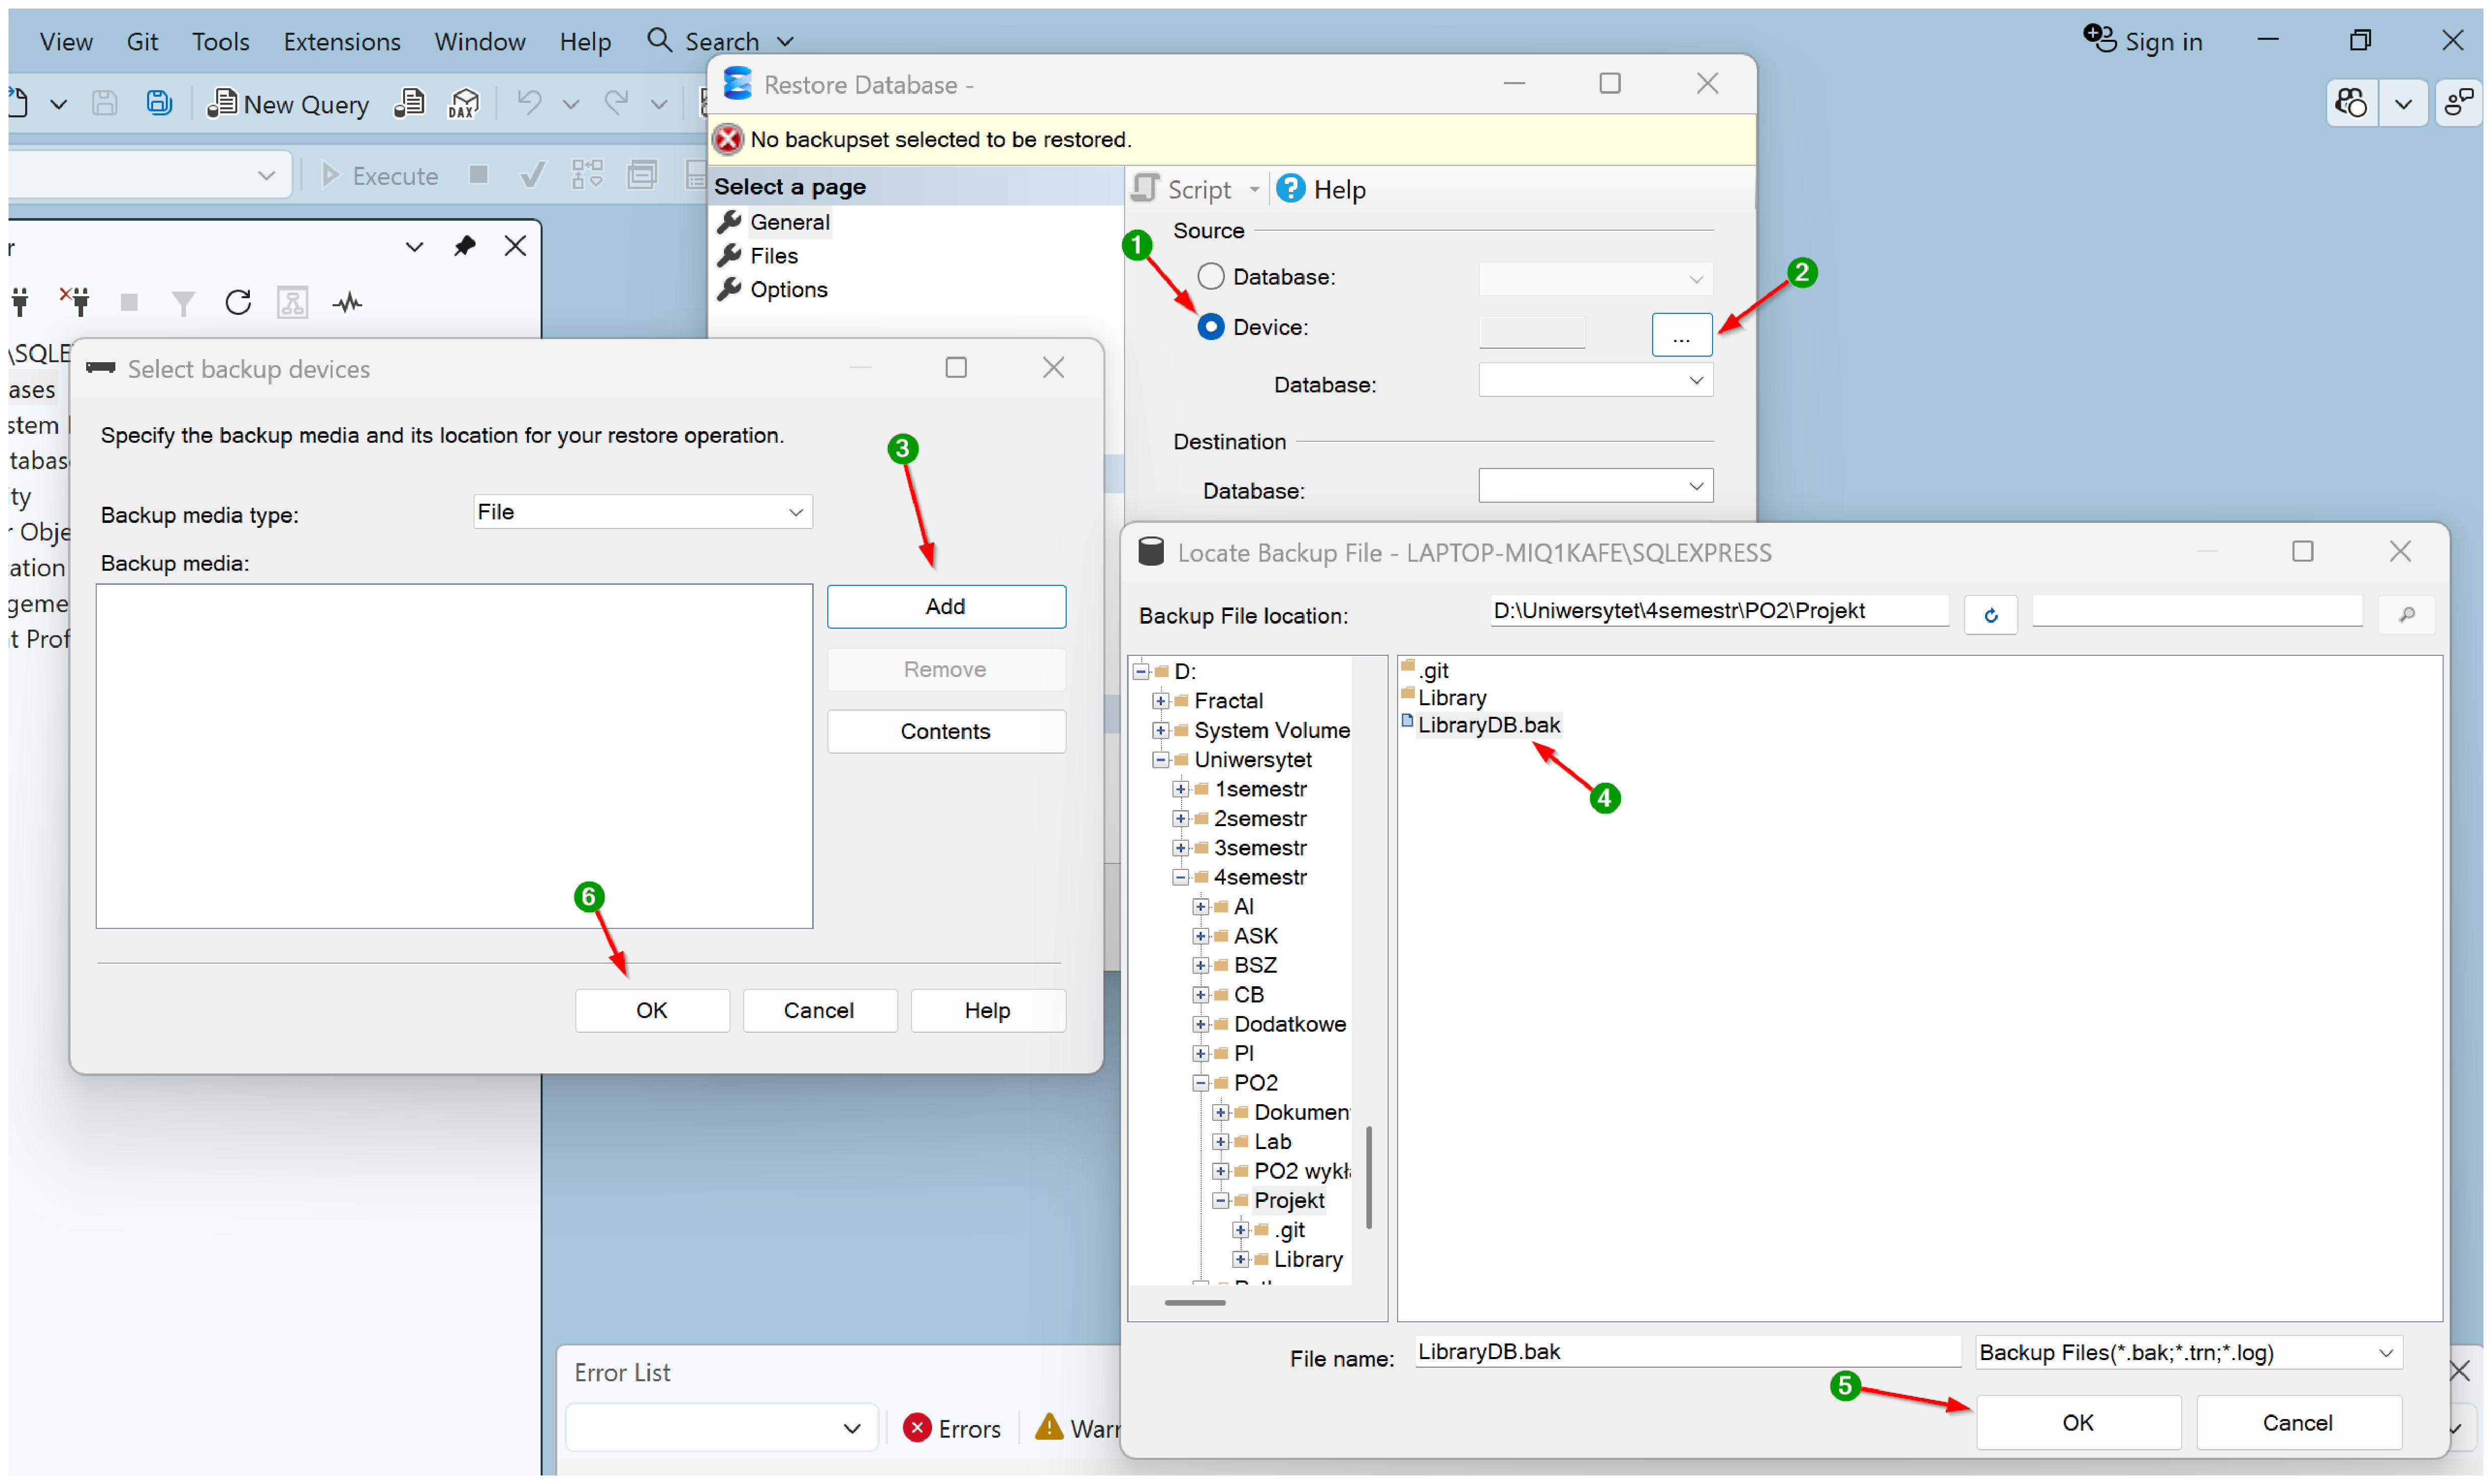
\includegraphics[width=0.8\linewidth]{figures/db2.eps}
        \caption{Przywracanie bazy danych z pliku backupu (cz. 2).\label{fig:db2_setup}}
    \end{figure}
    
    \begin{figure}[H]
        \centering
        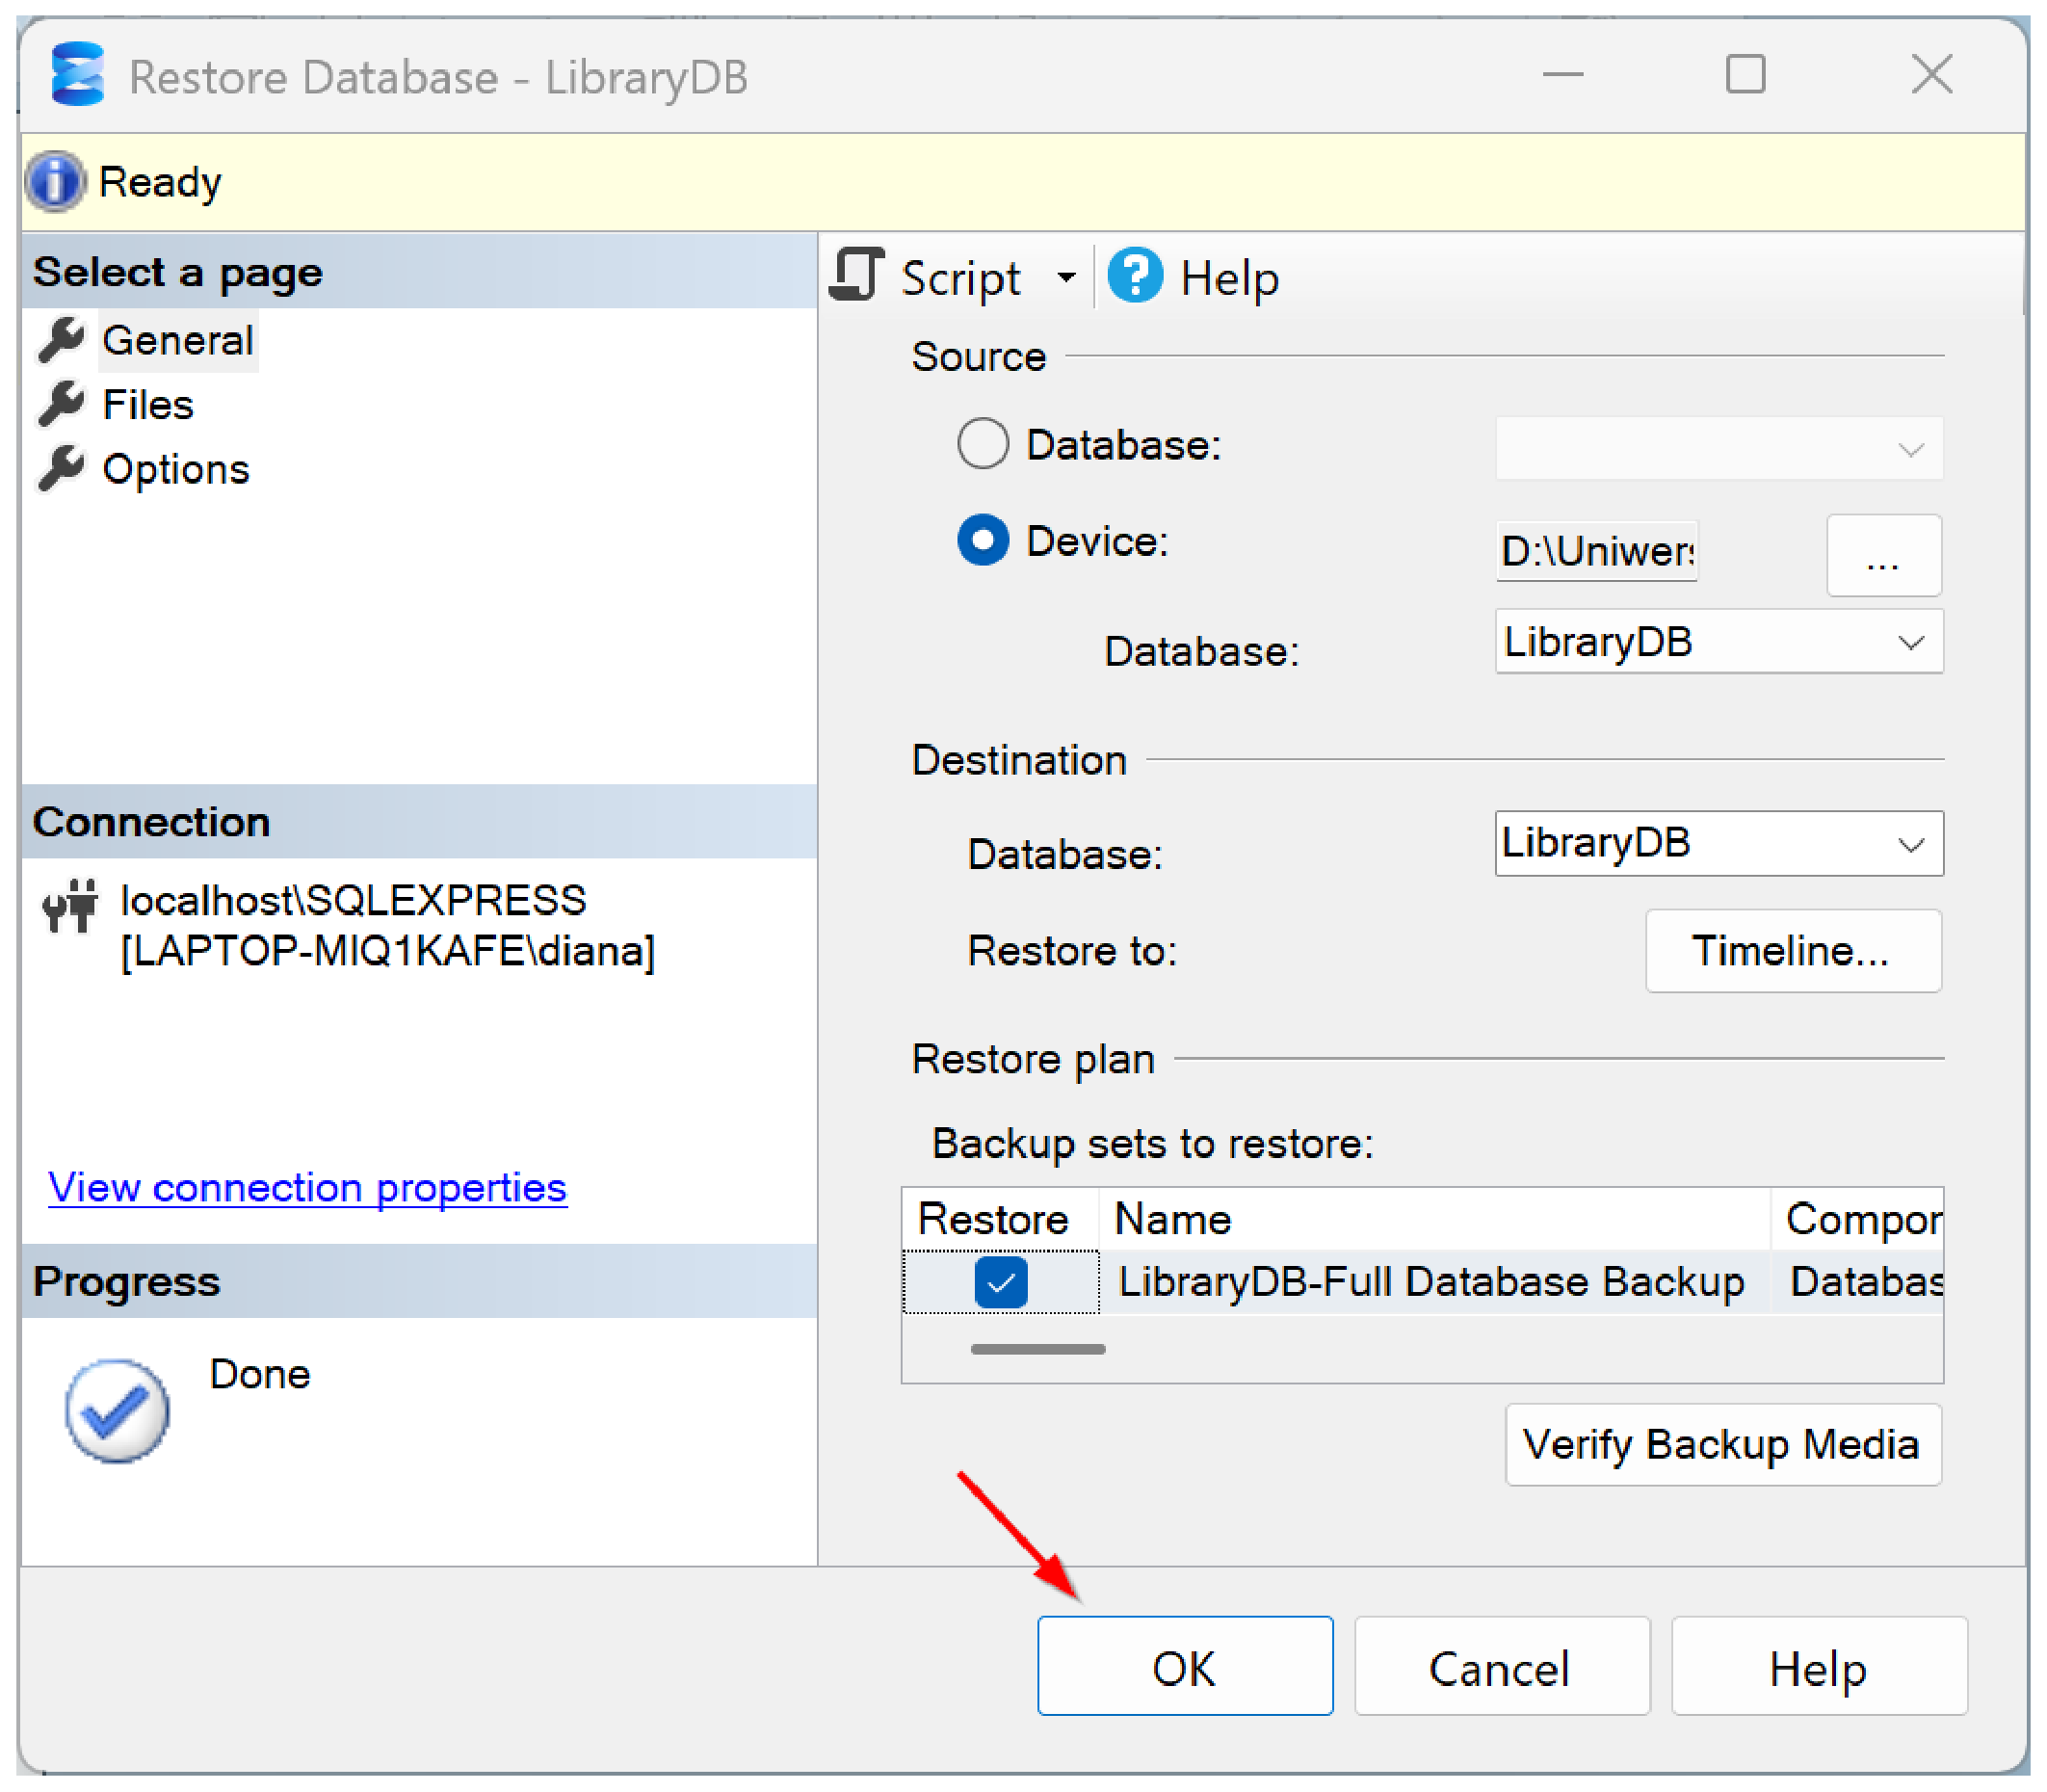
\includegraphics[width=0.5\linewidth]{figures/db3.eps}
        \caption{Przywracanie bazy danych z pliku backupu (cz. 3).\label{fig:db3_setup}}
    \end{figure}
    
    \item Otwórz rozwiązanie projektu C\# \texttt{Library.sln} w Visual Studio.
    \item Upewnij się, że masz zainstalowane i przywrócone wszystkie niezbędne pakiety NuGet wymagane do działania projektu. Są to następujące pakiety:
    \begin{itemize}
        \item \texttt{Microsoft.AspNetCore.Identity}
        \item \texttt{Microsoft.EntityFrameworkCore}
        \item \texttt{Microsoft.EntityFrameworkCore.SqlServer}
        \item \texttt{Microsoft.EntityFrameworkCore.Tools}
        \item \texttt{Microsoft.Extensions.Identity.Core}
    \end{itemize}
    
    \begin{figure}[H]
        \centering
        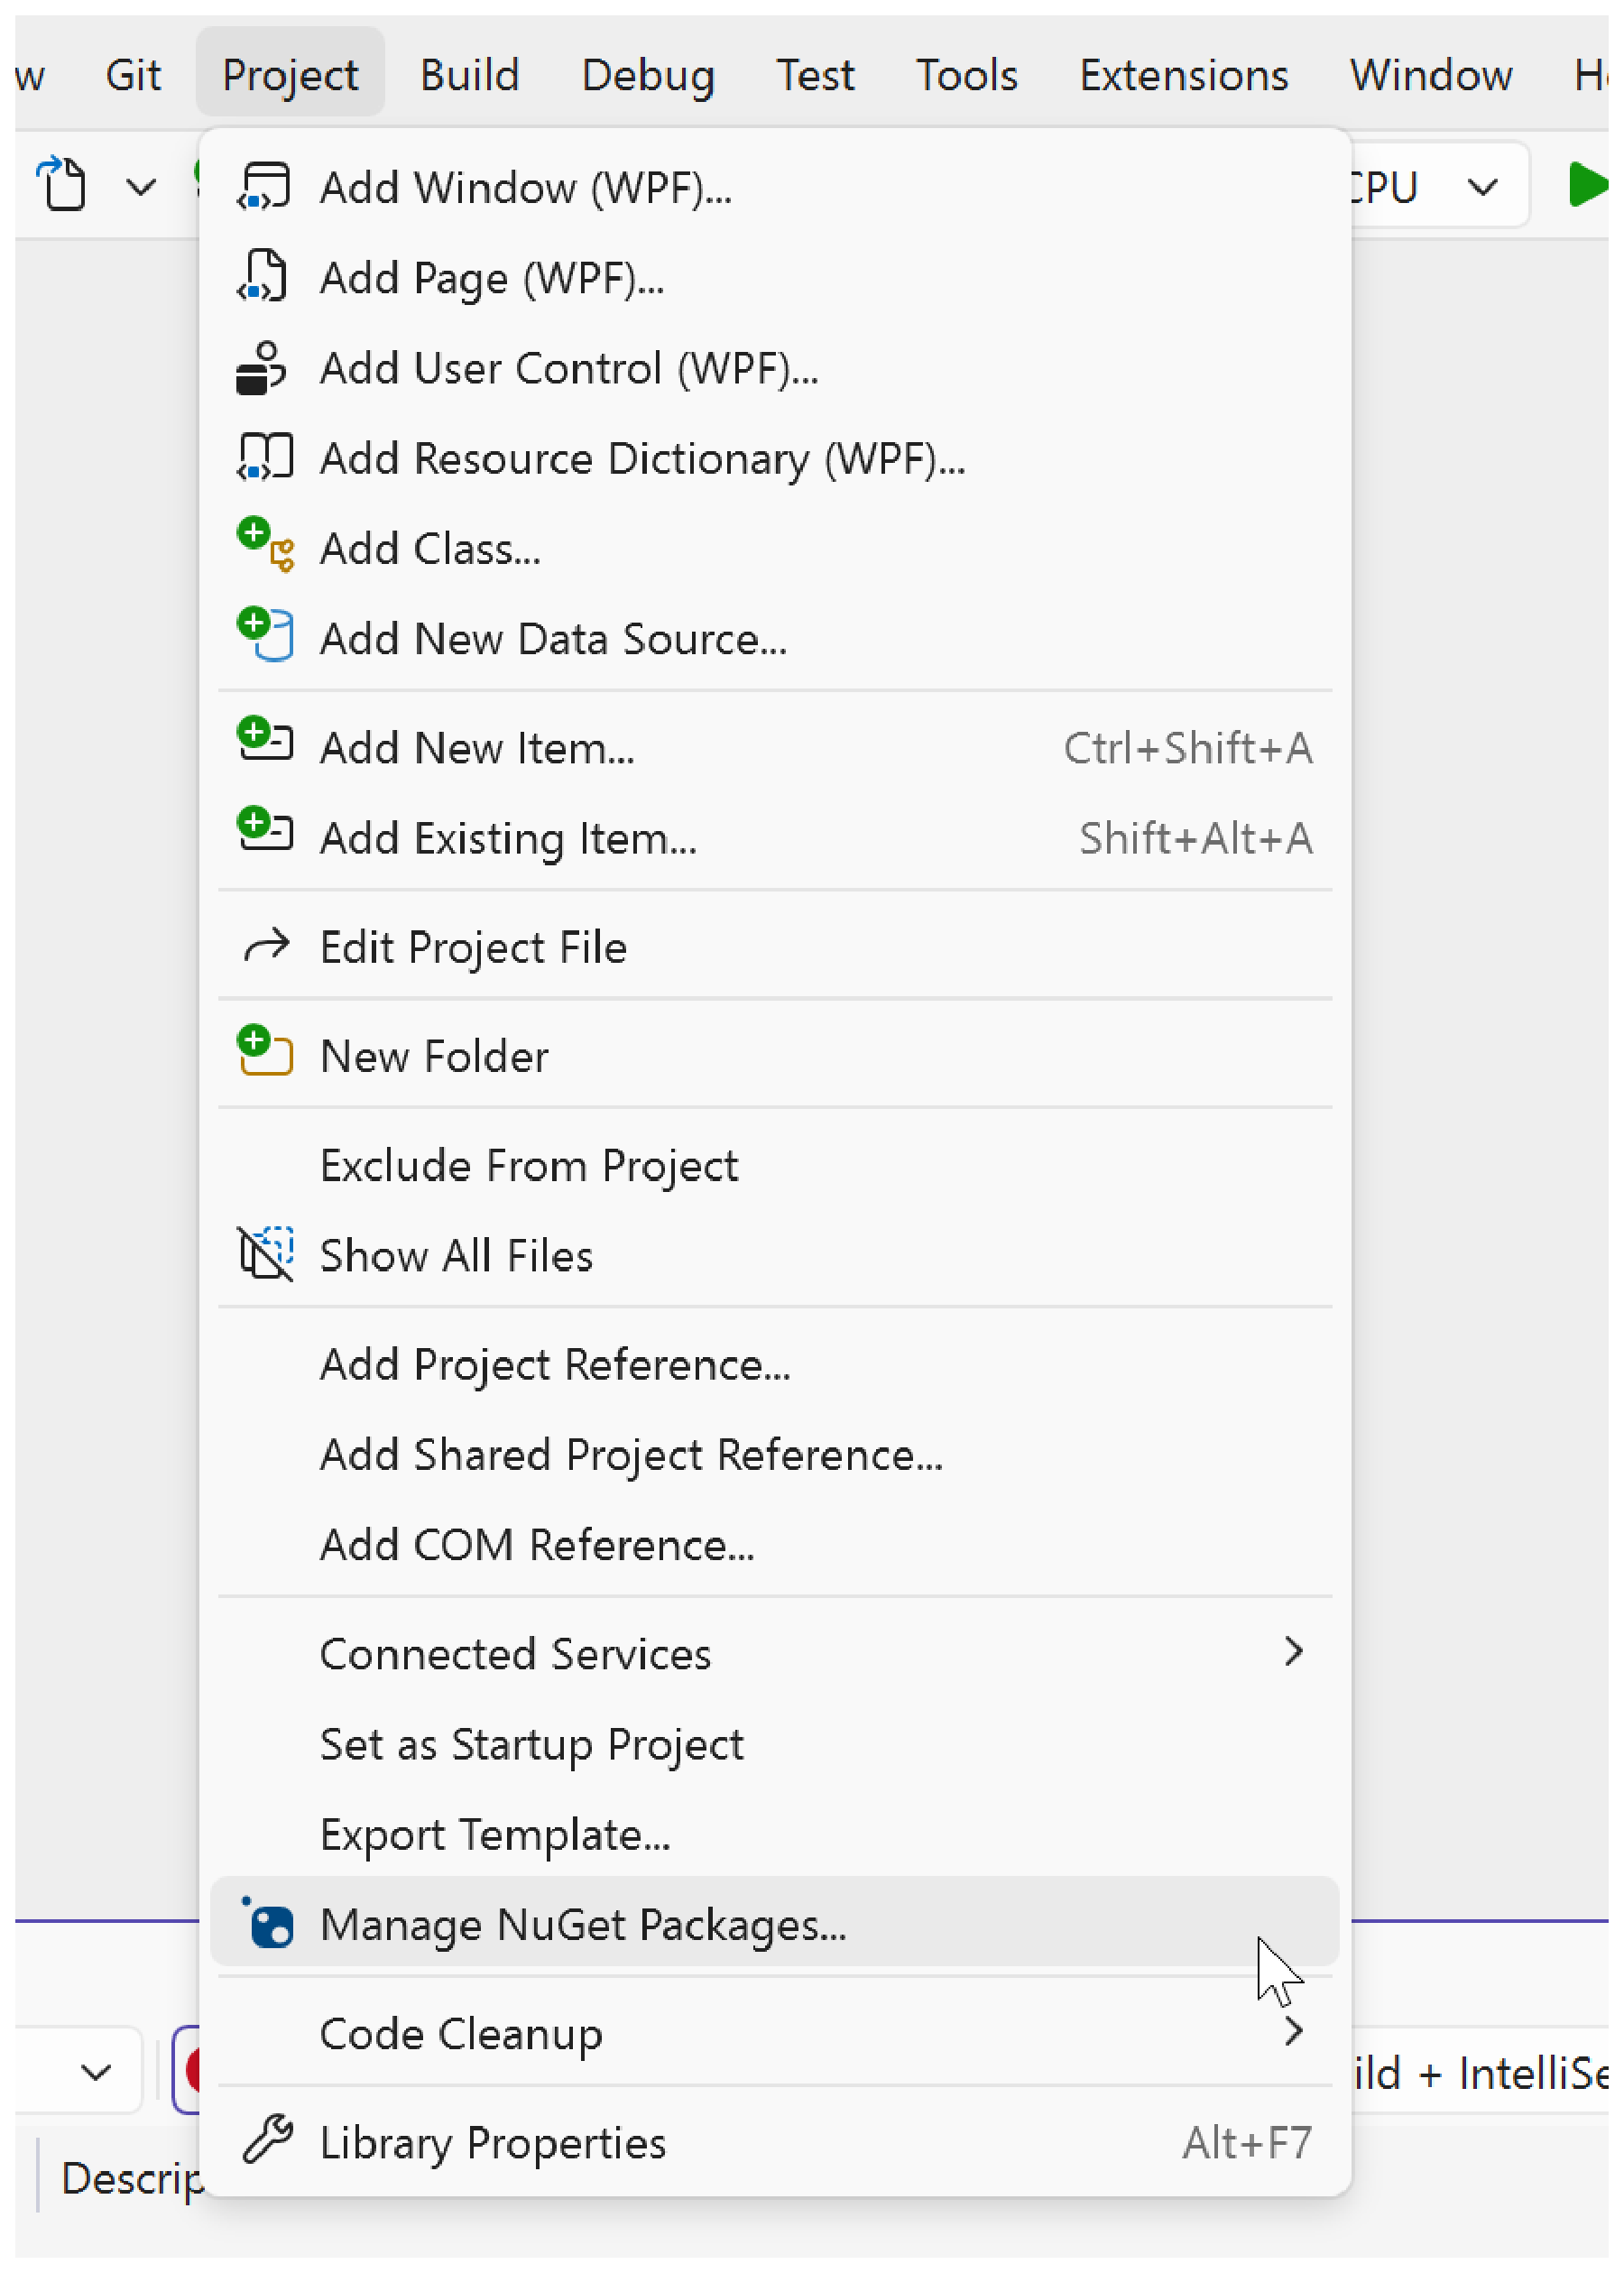
\includegraphics[width=0.5\linewidth]{figures/package1.eps}
        \caption{Zarządzanie pakietami NuGet - pobrane biblioteki (cz. 1).\label{fig:package1}}
    \end{figure}
    
    \begin{figure}[H]
        \centering
        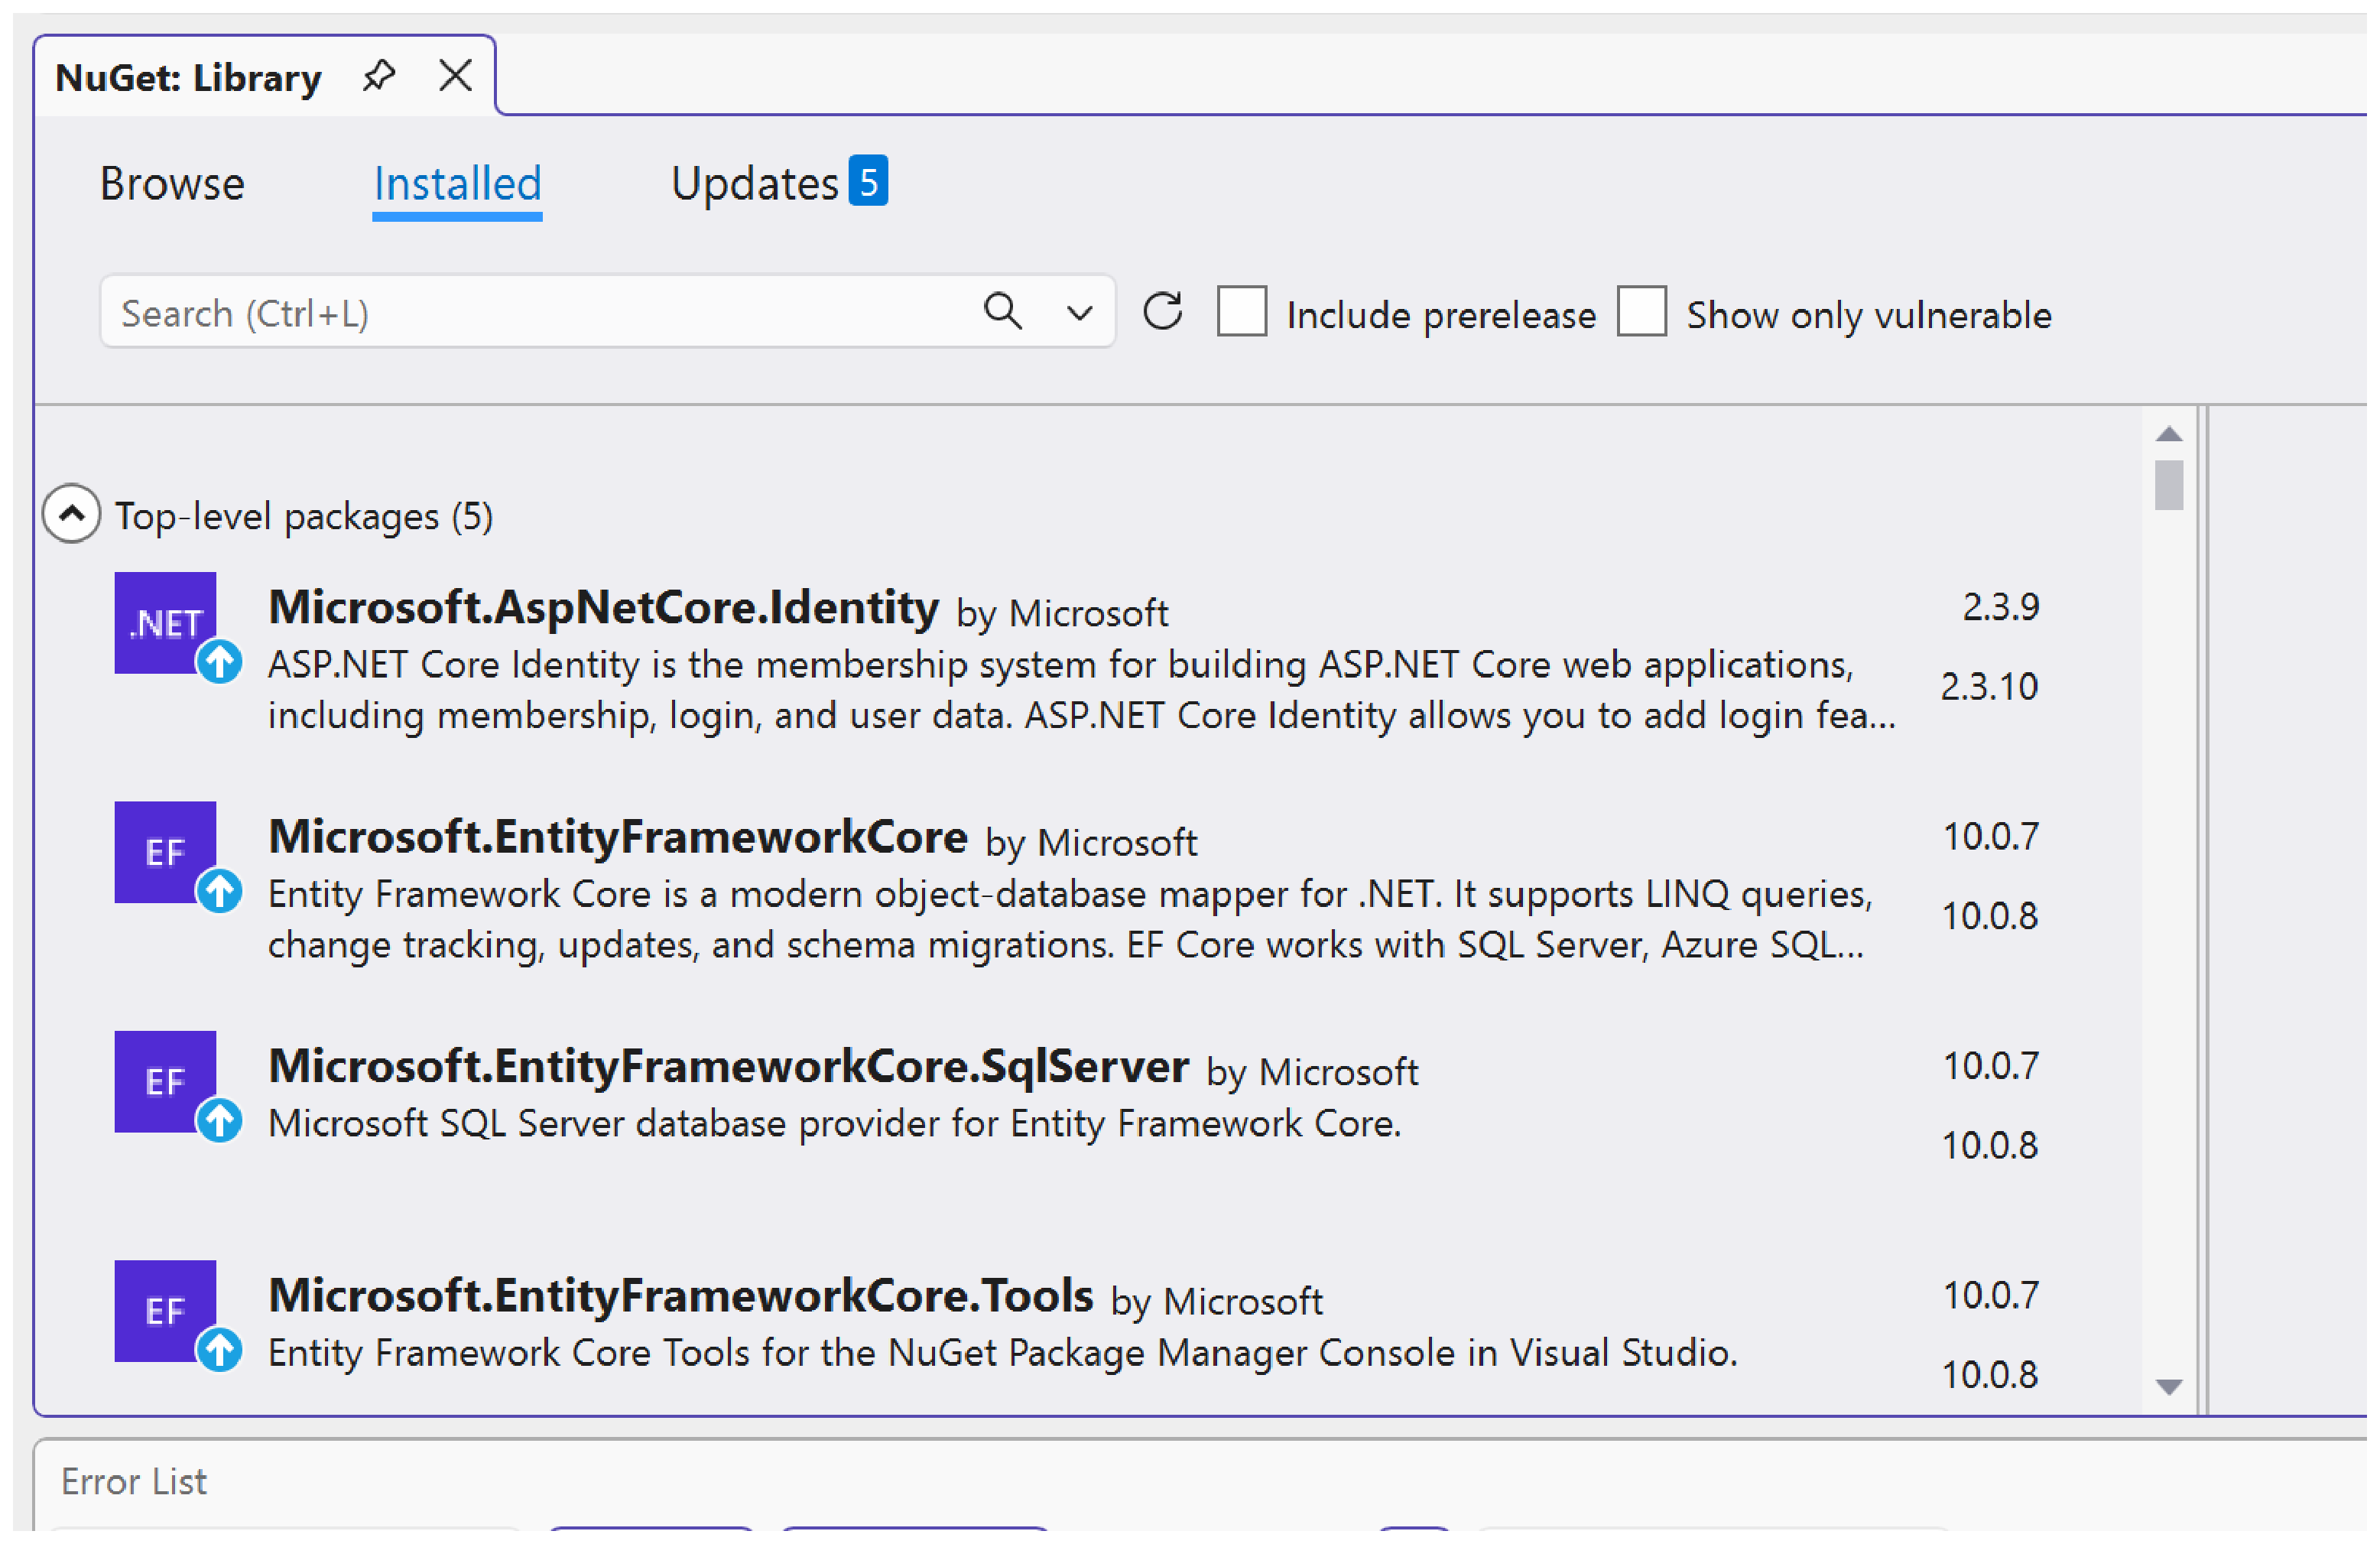
\includegraphics[width=0.8\linewidth]{figures/package2.eps}
        \caption{Zarządzanie pakietami NuGet - pobrane biblioteki (cz. 2).\label{fig:package2}}
    \end{figure}
    
    \item Zbuduj projekt i uruchom (Start / F5).
\end{enumerate}

\textbf{Dane testowe}:
Aby przetestować działanie poszczególnych ról w systemie, po zaimportowaniu bazy danych można zalogować się używając poniższych poświadczeń:
\begin{itemize}
    \item Bibliotekarz: Login: \texttt{admin}, Hasło: \texttt{admin1234}
    \item Czytelnik: Login: \texttt{anna}, Hasło: \texttt{anna1234}
\end{itemize}

\chapter{Prezentacja warstwy użytkowej projektu}
Graficzny interfejs użytkownika (GUI) został zaprojektowany w technologii WPF z naciskiem na przejrzystość, ergonomię i intuicyjną obsługę. Przepływ pracy (User Flow) w aplikacji rozpoczyna się od autoryzacji, a następnie kieruje użytkownika do dedykowanego panelu w zależności od nadanych mu uprawnień.

Pierwszym oknem dialogowym, z którym styka się użytkownik, jest ekran logowania. Pozwala on na wprowadzenie nazwy użytkownika i hasła, weryfikowanych następnie w bazie danych. Okno zawiera również przycisk pozwalający na przejście do formularza utworzenia nowego konta.
\begin{figure}[H]
    \centering
    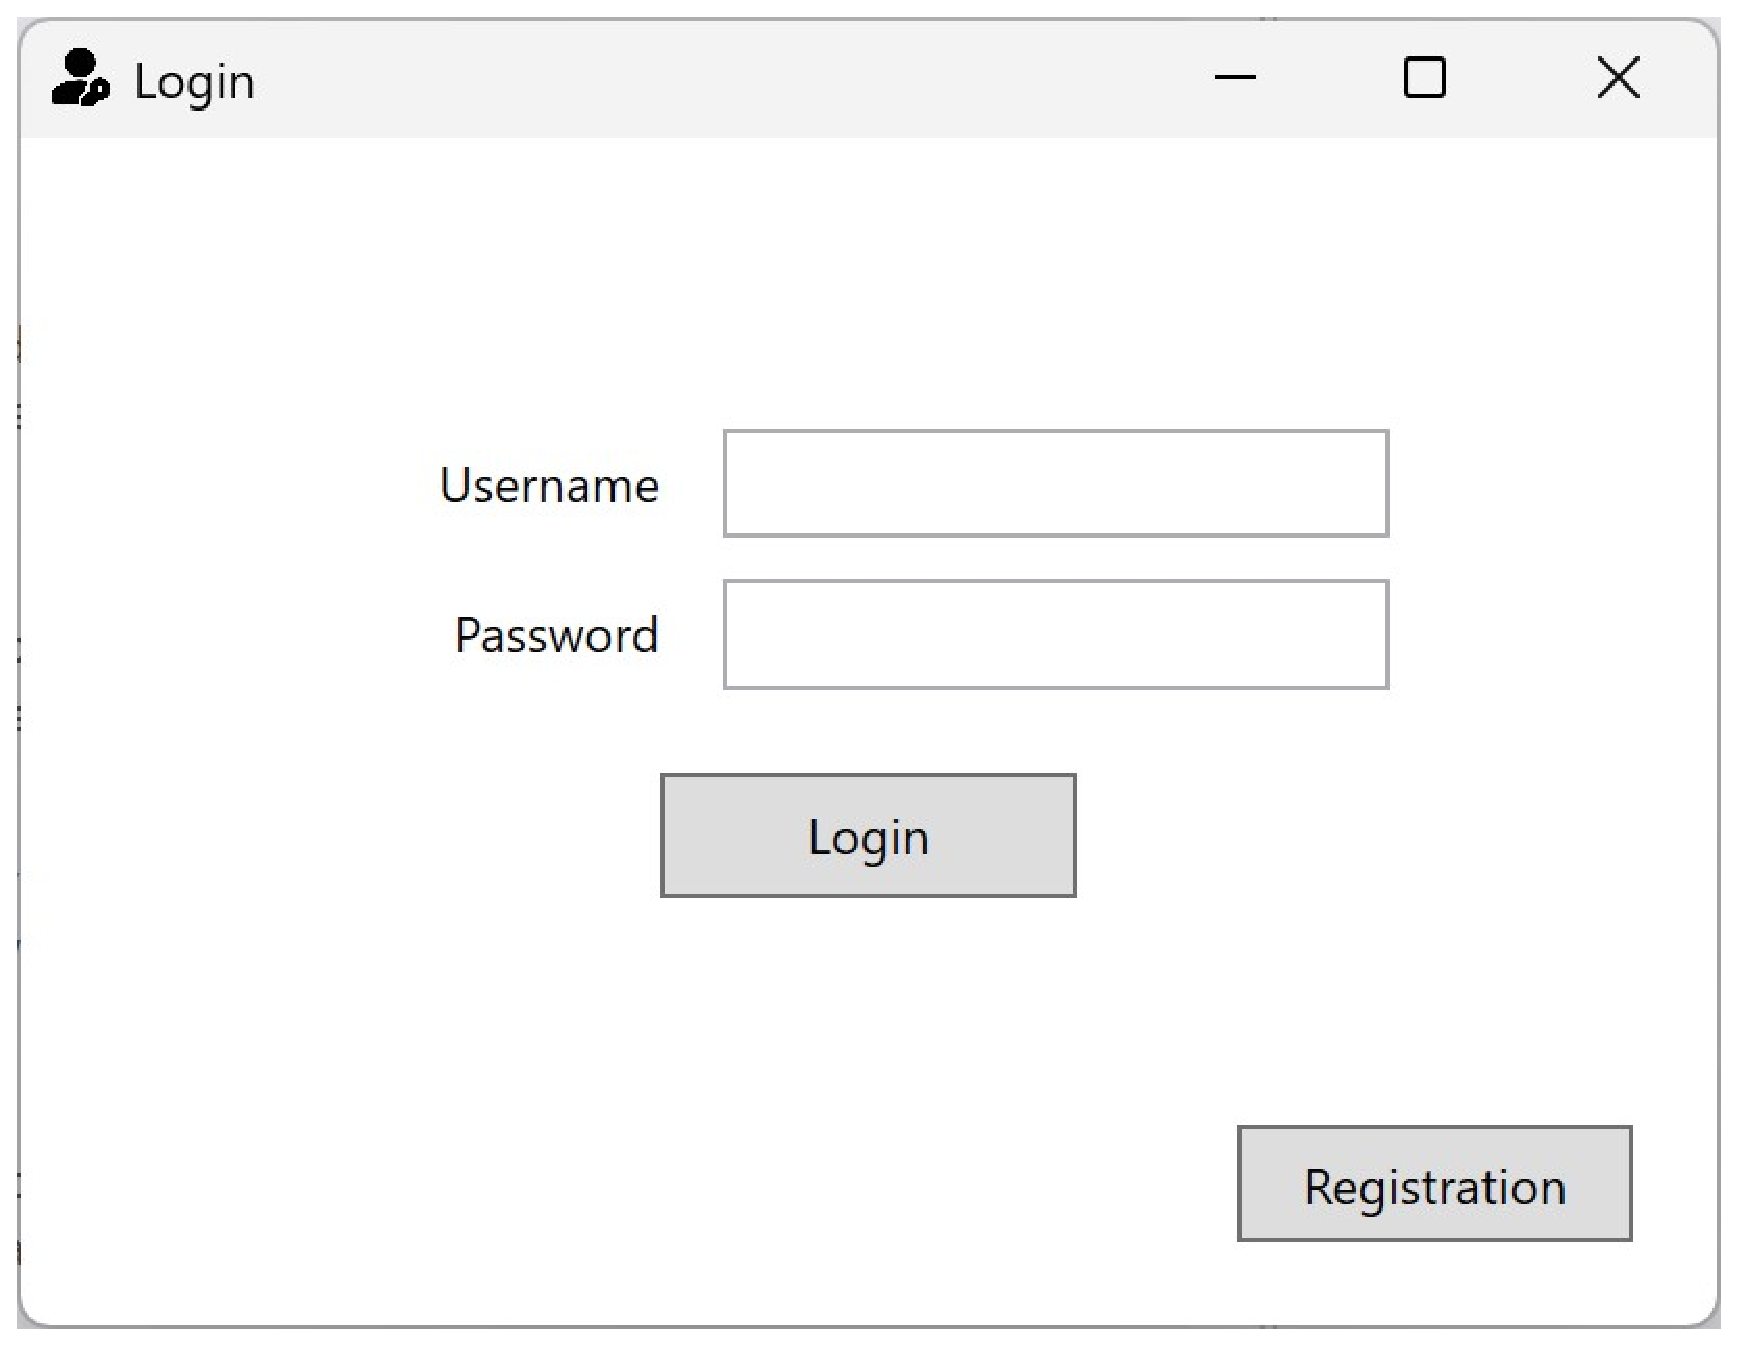
\includegraphics[width=0.6\linewidth]{figures/show/show1.eps}
    \caption{Ekran logowania do systemu.\label{fig:ui_login}}
\end{figure}

W przypadku wyboru opcji założenia konta, aplikacja przenosi do panelu rejestracji. 
Wymaga on uzupełnienia podstawowych danych osobowych oraz ustalenia własnych danych dostępowych do systemu.
\begin{figure}[H]
    \centering
    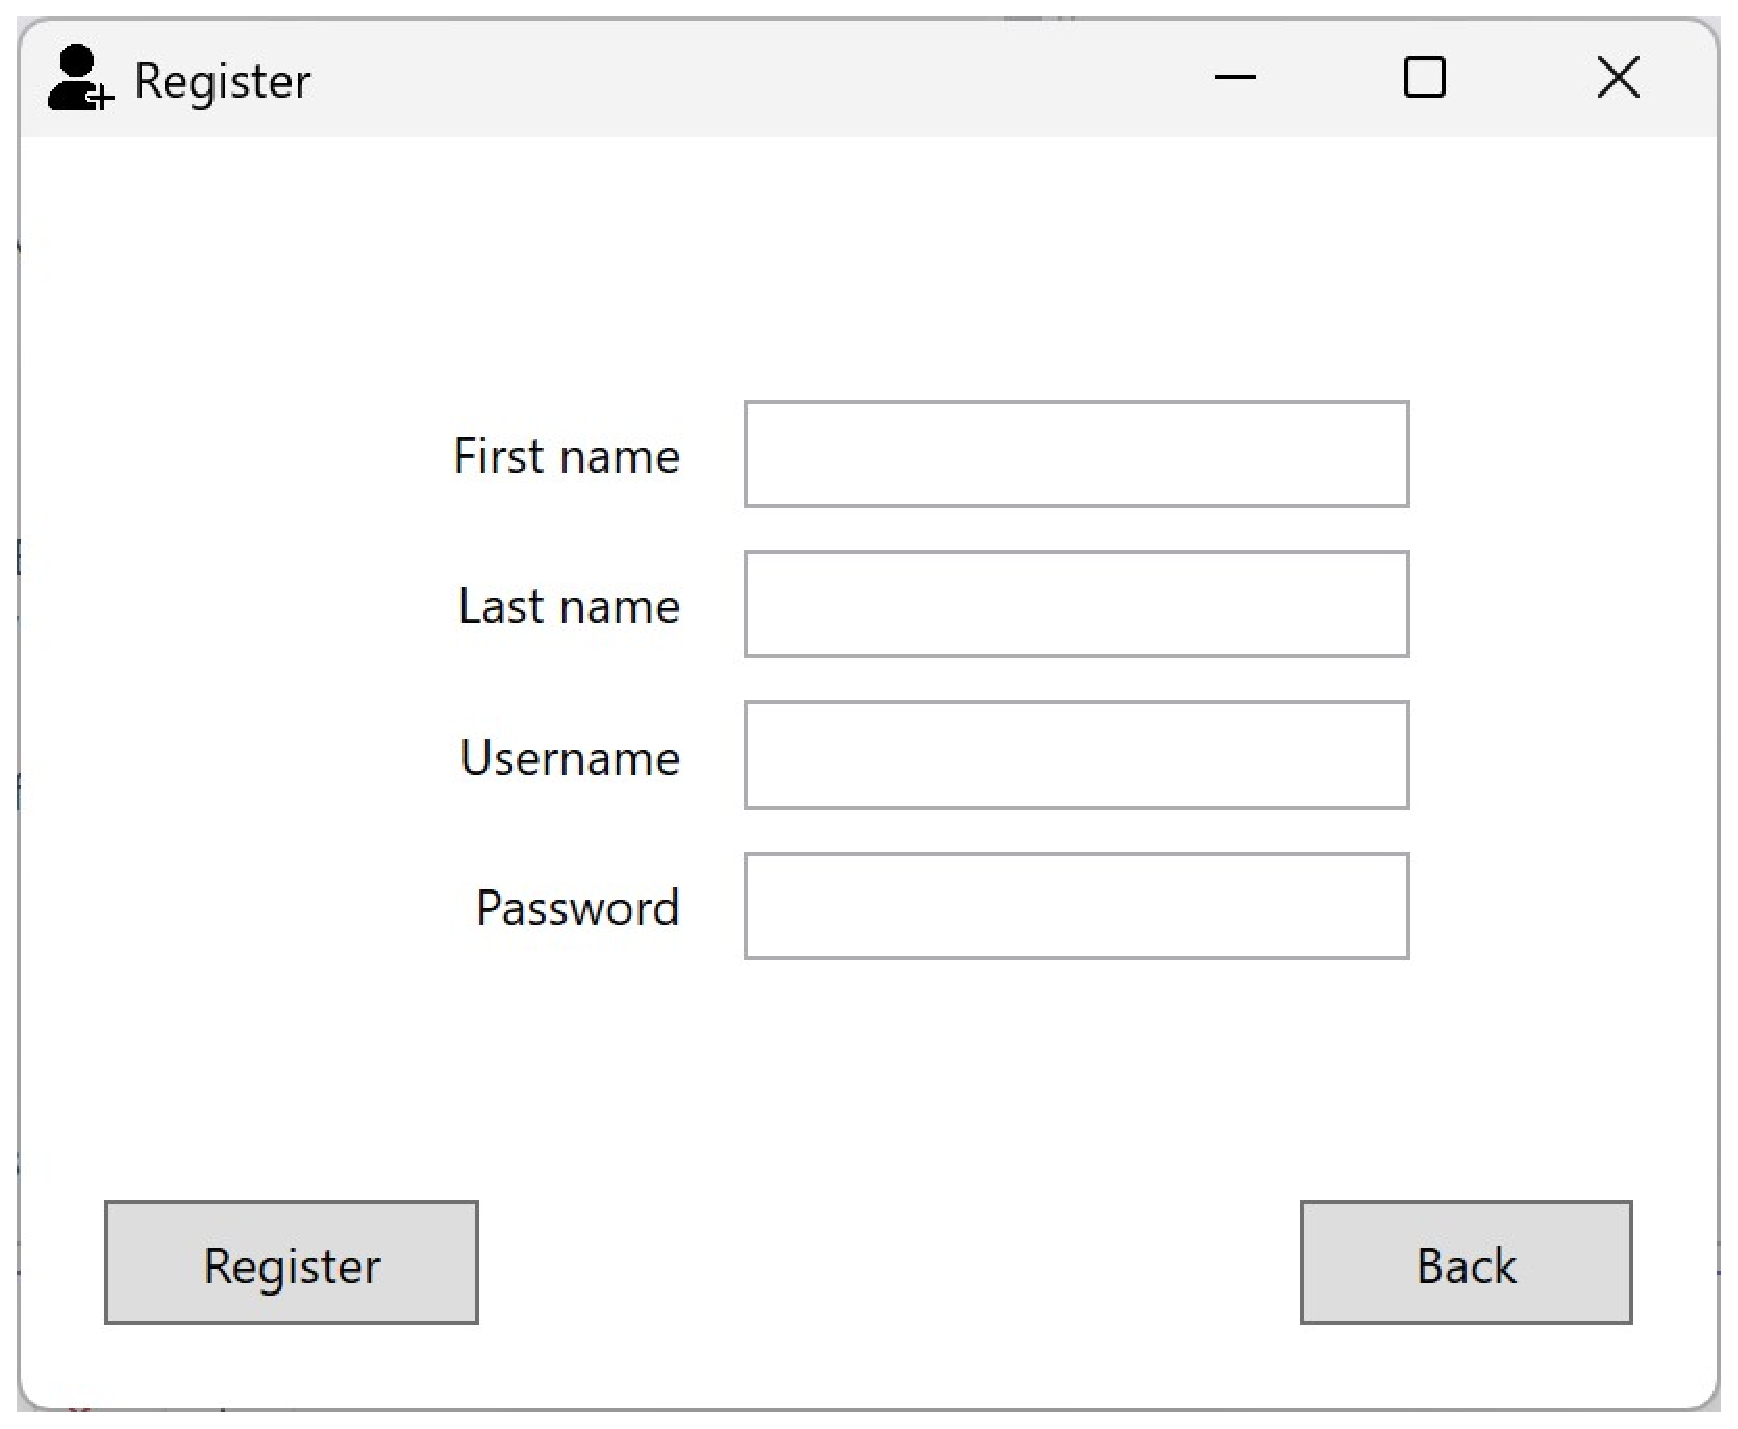
\includegraphics[width=0.6\linewidth]{figures/show/show2.eps}
    \caption{Ekran rejestracji nowego użytkownika.\label{fig:ui_register}}
\end{figure}

Po pomyślnym zalogowaniu z uprawnieniami administracyjnymi (jako bibliotekarz), użytkownikowi ukazuje się główne menu nawigacyjne. Udostępnia ono scentralizowany dostęp do kluczowych procesów systemu, pozwalając na przejście do zarządzania zasobami biblioteki (\textit{Book catalog}), kontrolowania użytkowników (\textit{View user list}) oraz zmiany hasła. 

Istotnym elementem tego widoku jest moduł \textit{Data Backup \& Exchange} umieszczony w dolnej części interfejsu. Umożliwia on administratorowi wybiórcze zarządzanie kopiami zapasowymi poszczególnych danych (za pomocą pól wyboru dla tabel: Loans, Books, Users), a następnie wyeksportowanie ich do zewnętrznych plików lub zaimportowanie z powrotem w celu odtworzenia stanu biblioteki.
\begin{figure}[H]
    \centering
    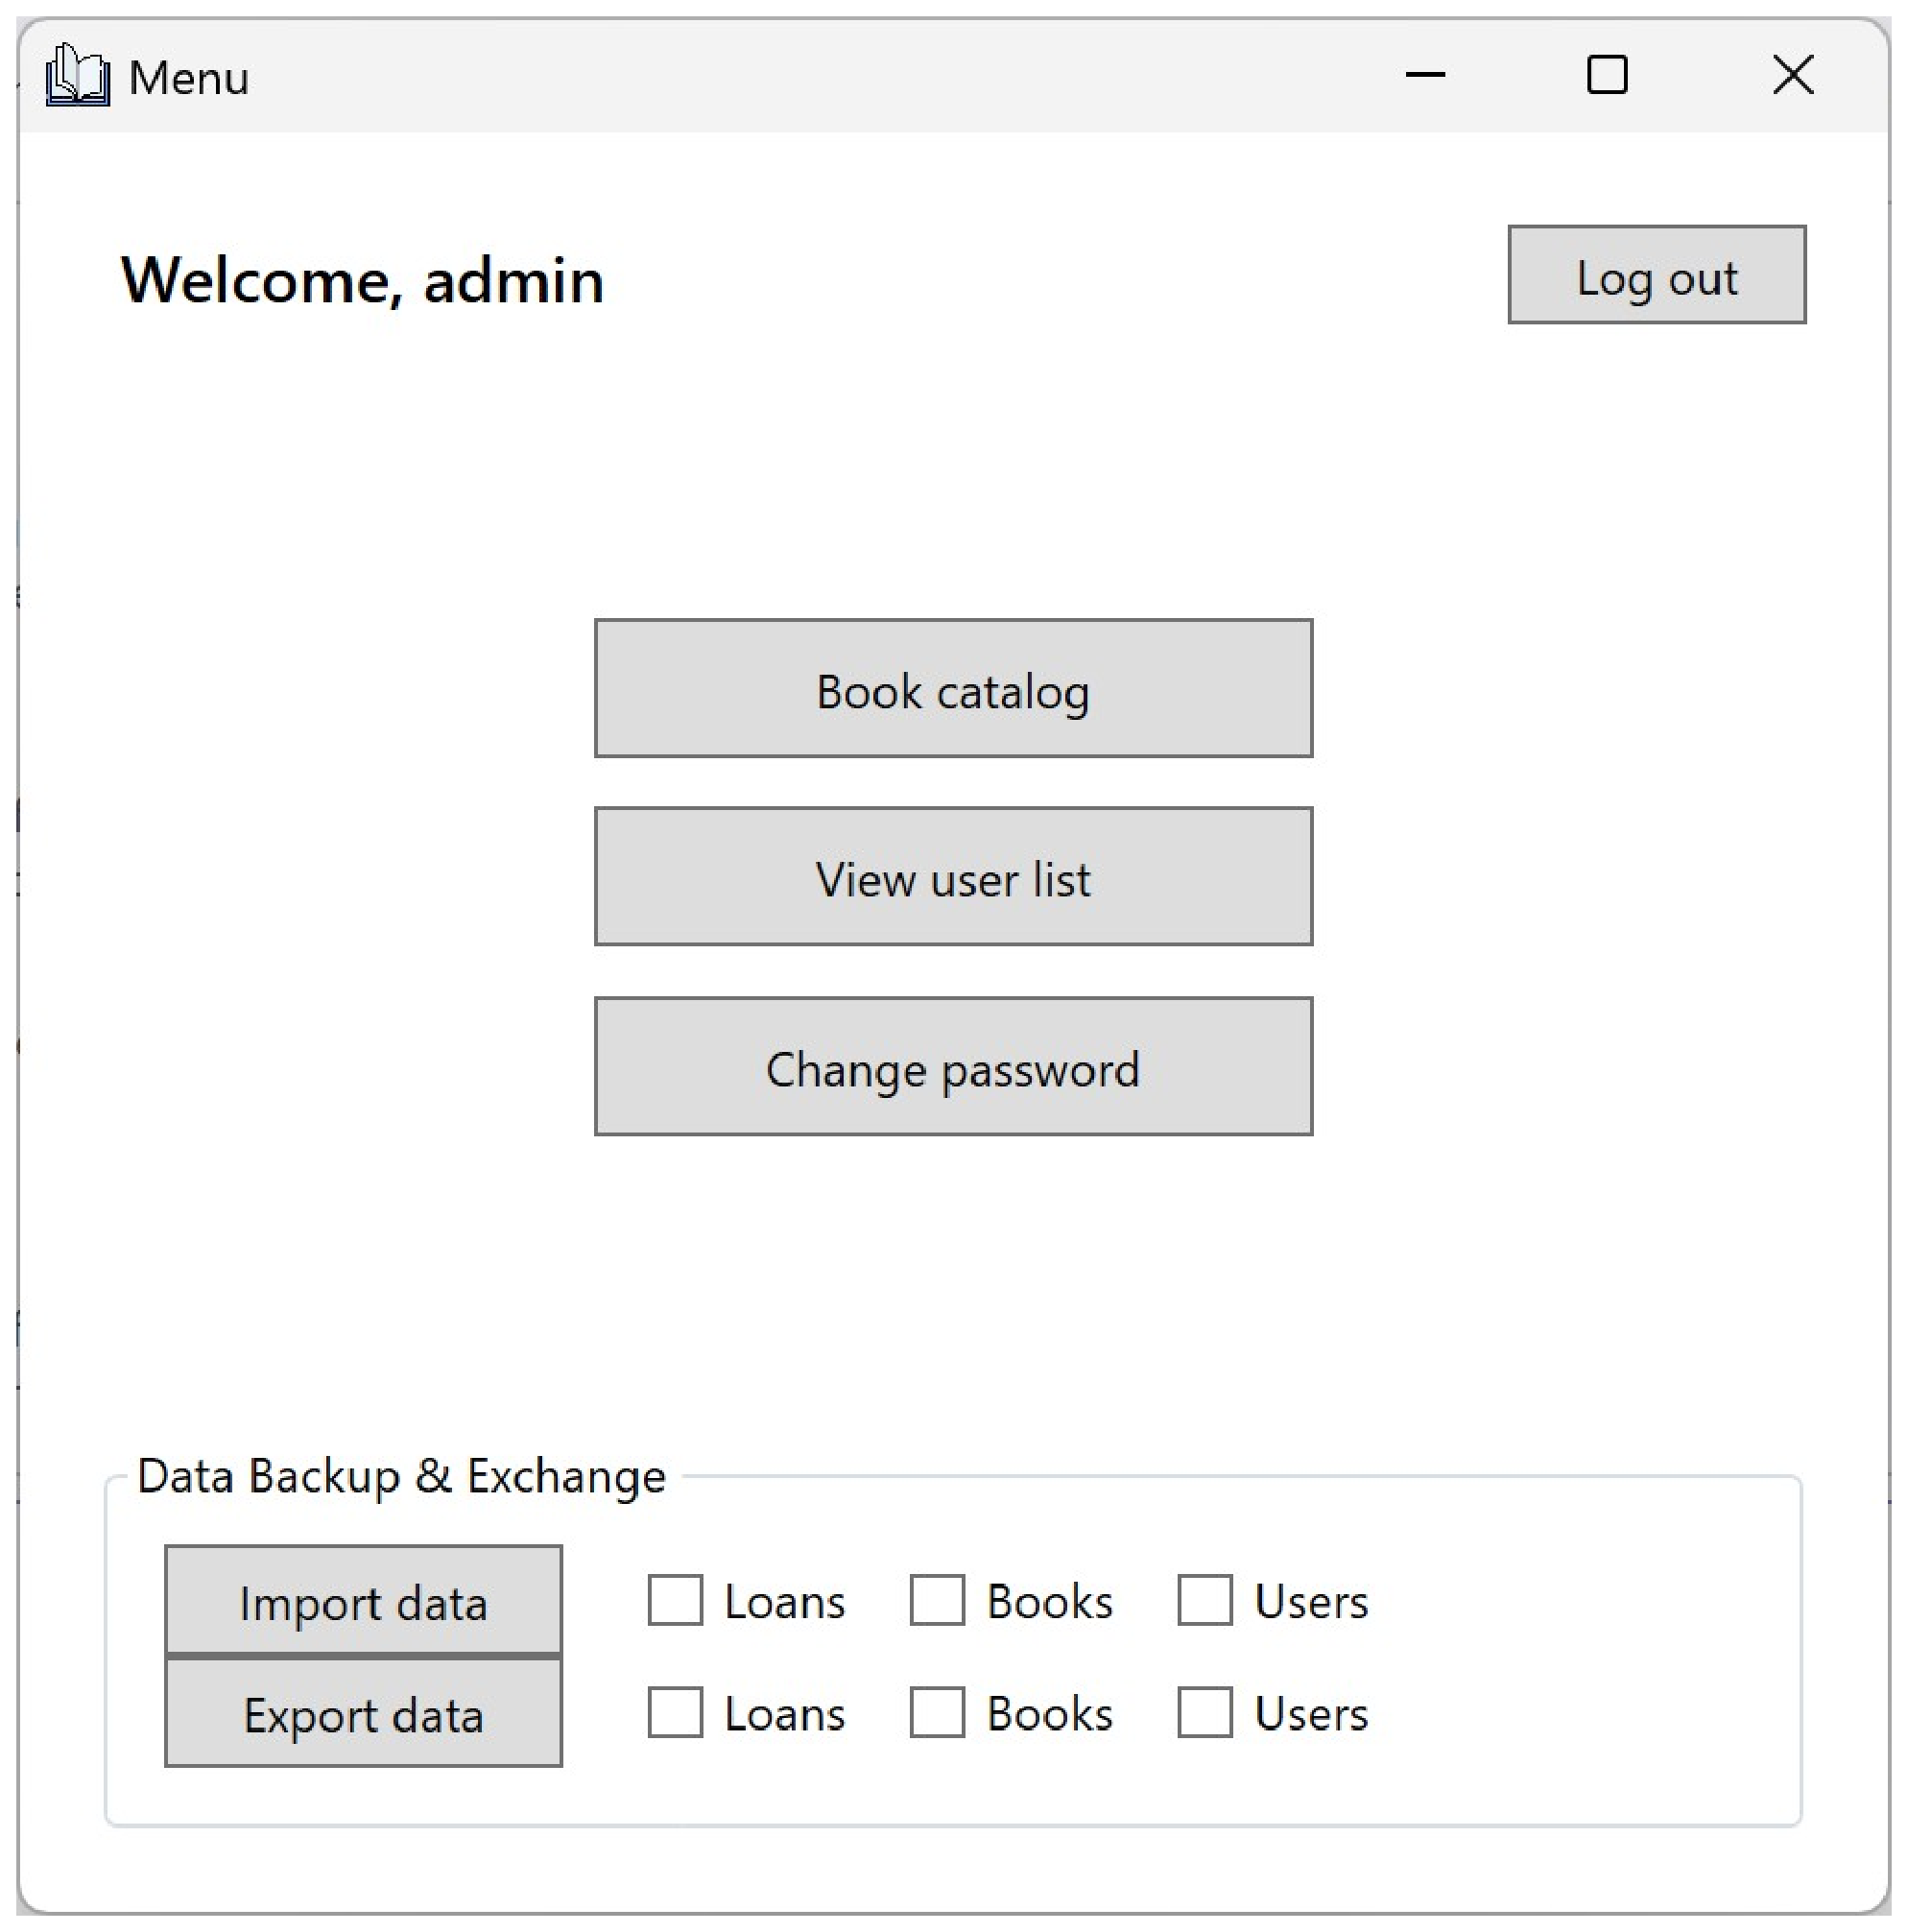
\includegraphics[width=0.6\linewidth]{figures/show/show3.eps}
    \caption{Główne menu administratora z panelem zarządzania kopiami zapasowymi.\label{fig:ui_admin_menu}}
\end{figure}

Kluczowym modułem dla bibliotekarza jest zarządzanie zbiorami, dostępne pod opcją \textit{Book catalog}. Wyświetla ono czytelną tabelę ze wszystkimi pozycjami w bibliotece. Umożliwia zaawansowane wyszukiwanie książek (po frazie zawartej we wszystkich polach, konkretnym tytule lub nazwisku autora) oraz filtrowanie wyników na podstawie wybranej kategorii. Z tego poziomu administrator ma również kontrolę nad zasobami, korzystając z umieszczonych na dole przycisków służących do dodawania, edycji lub usuwania zaznaczonej pozycji.
\begin{figure}[H]
    \centering
    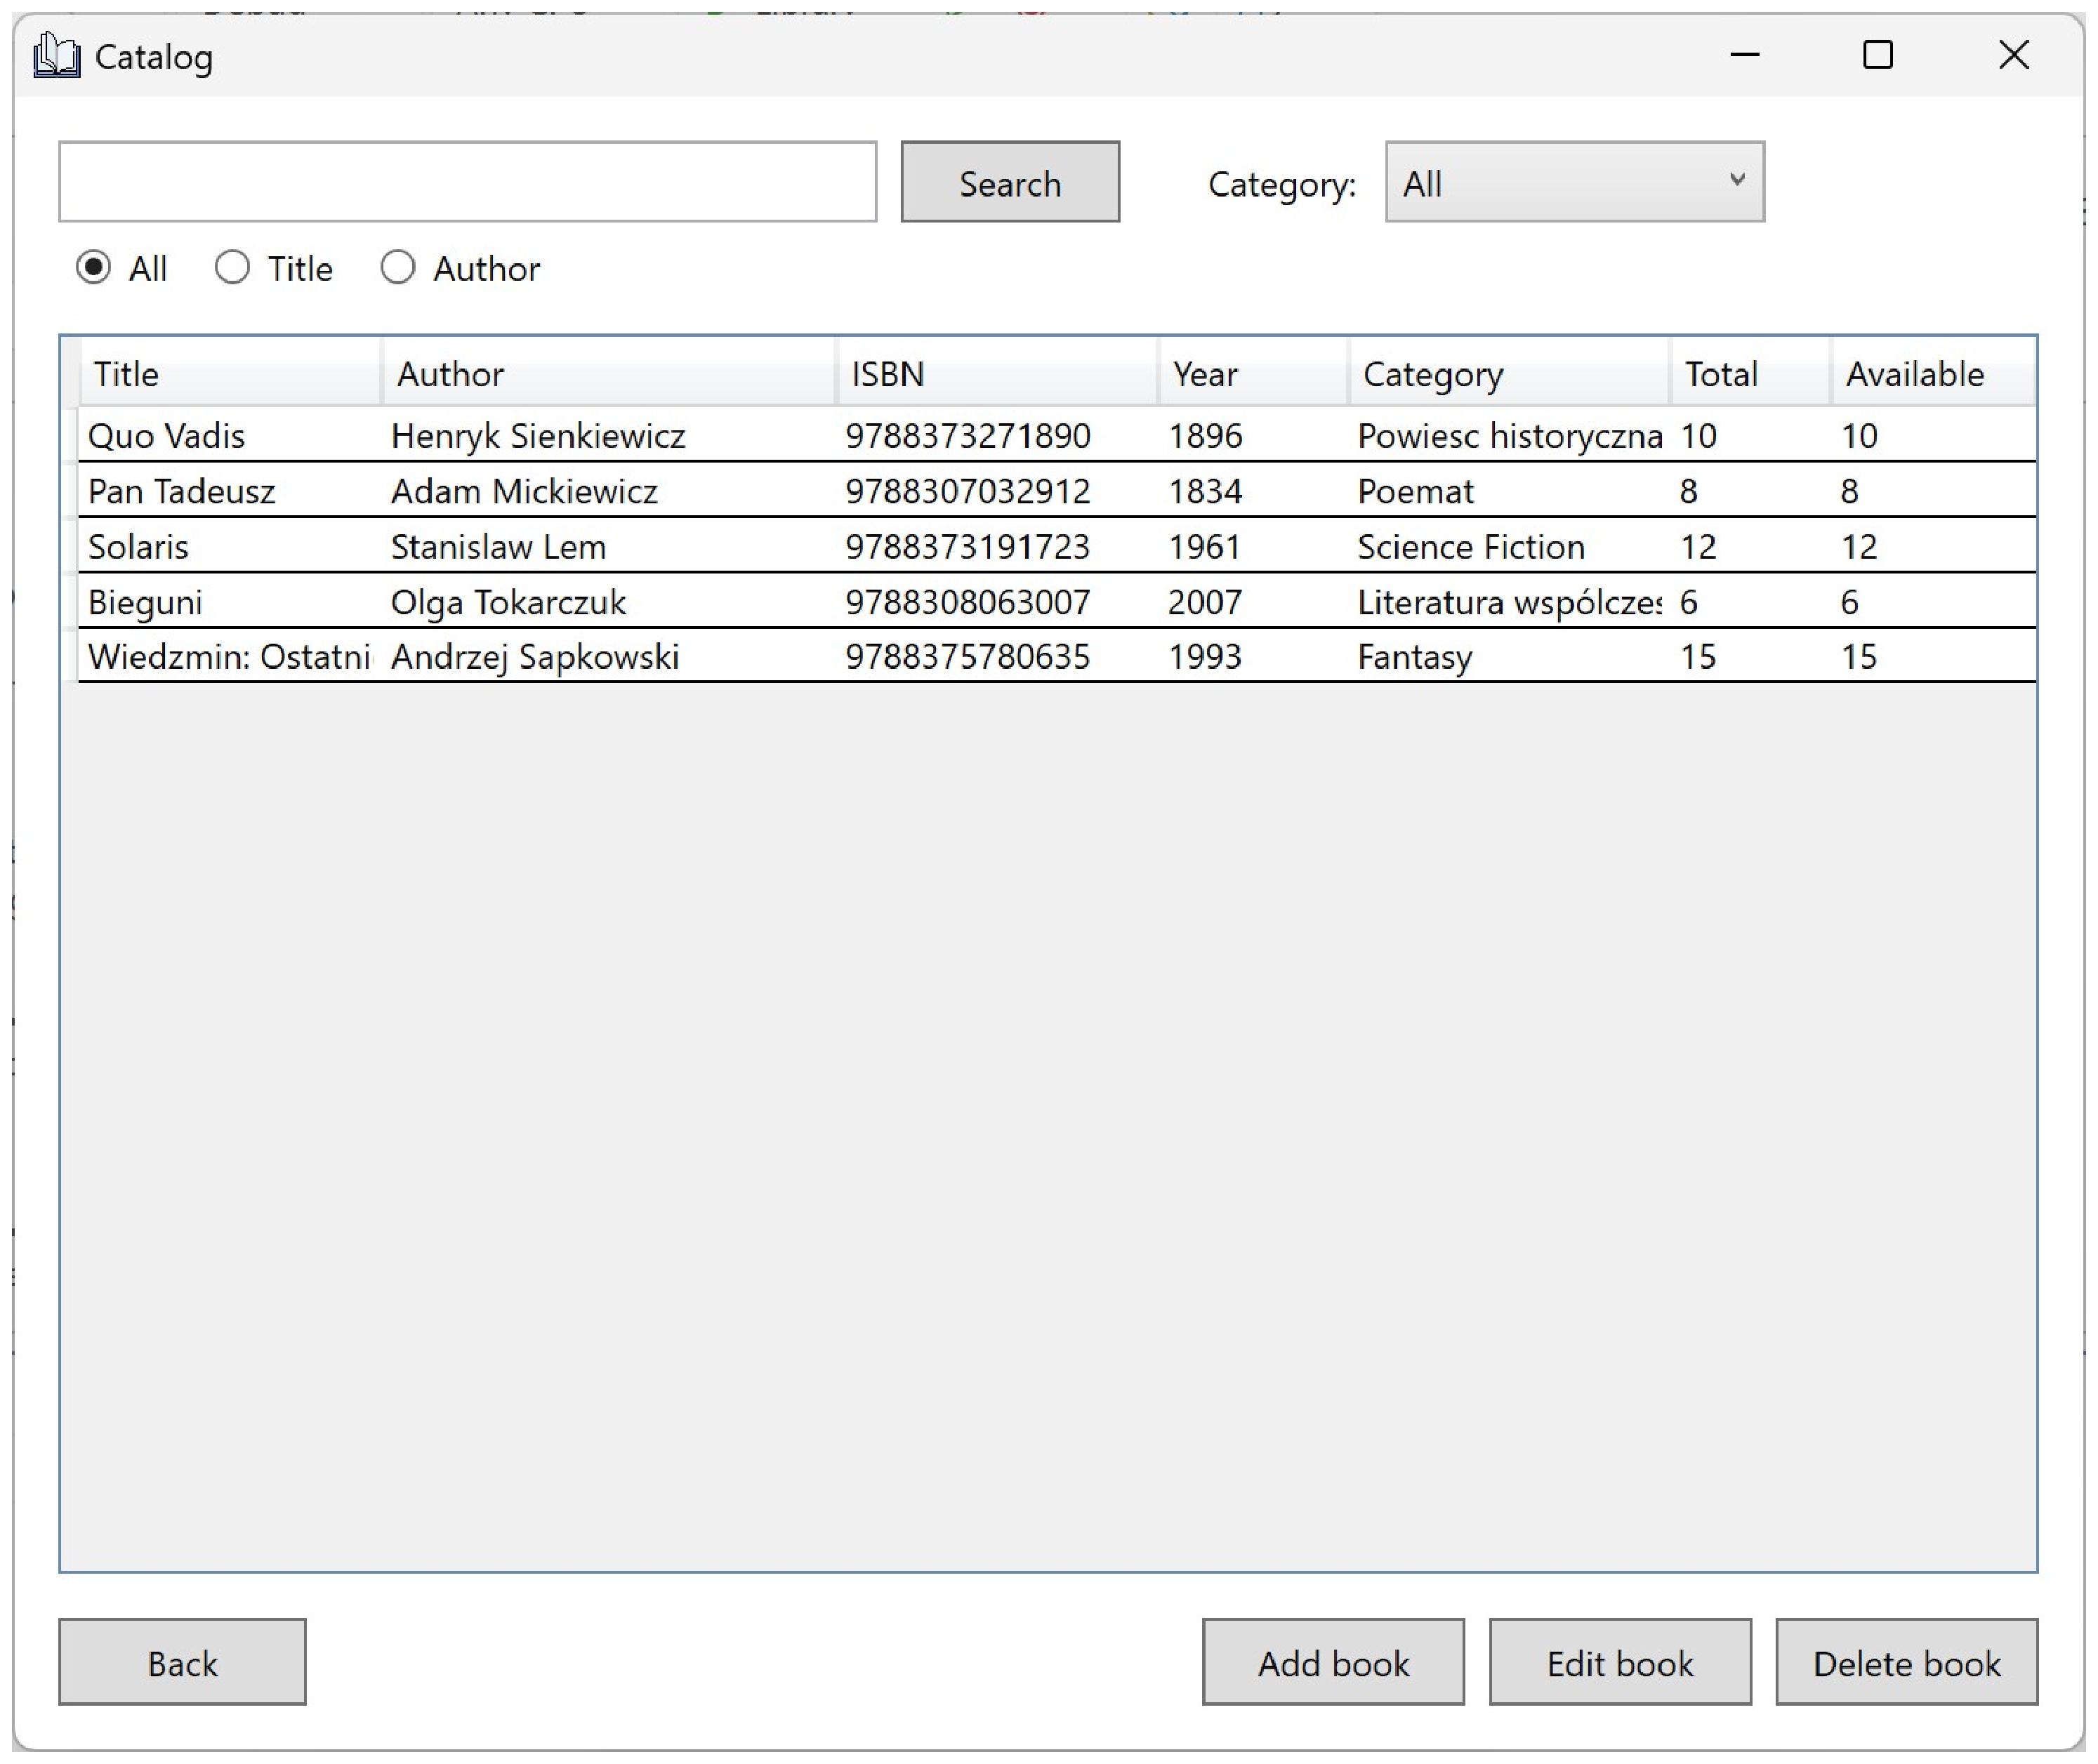
\includegraphics[width=0.8\linewidth]{figures/show/show4.eps}
    \caption{Katalog książek z wyszukiwarką i opcjami zarządzania (widok bibliotekarza).\label{fig:ui_catalog}}
\end{figure}

Kliknięcie przycisku dodawania nowej książki otwiera dedykowany formularz. Bibliotekarz musi wprowadzić niezbędne informacje ewidencyjne, takie jak: tytuł, autor, kategoria (z możliwością wyboru istniejącej z rozwijanej listy lub wpisania nowej poprzez tryb \textit{New}), numer ISBN, rok publikacji oraz całkowitą liczbę wprowadzanych na stan egzemplarzy.
\begin{figure}[H]
    \centering
    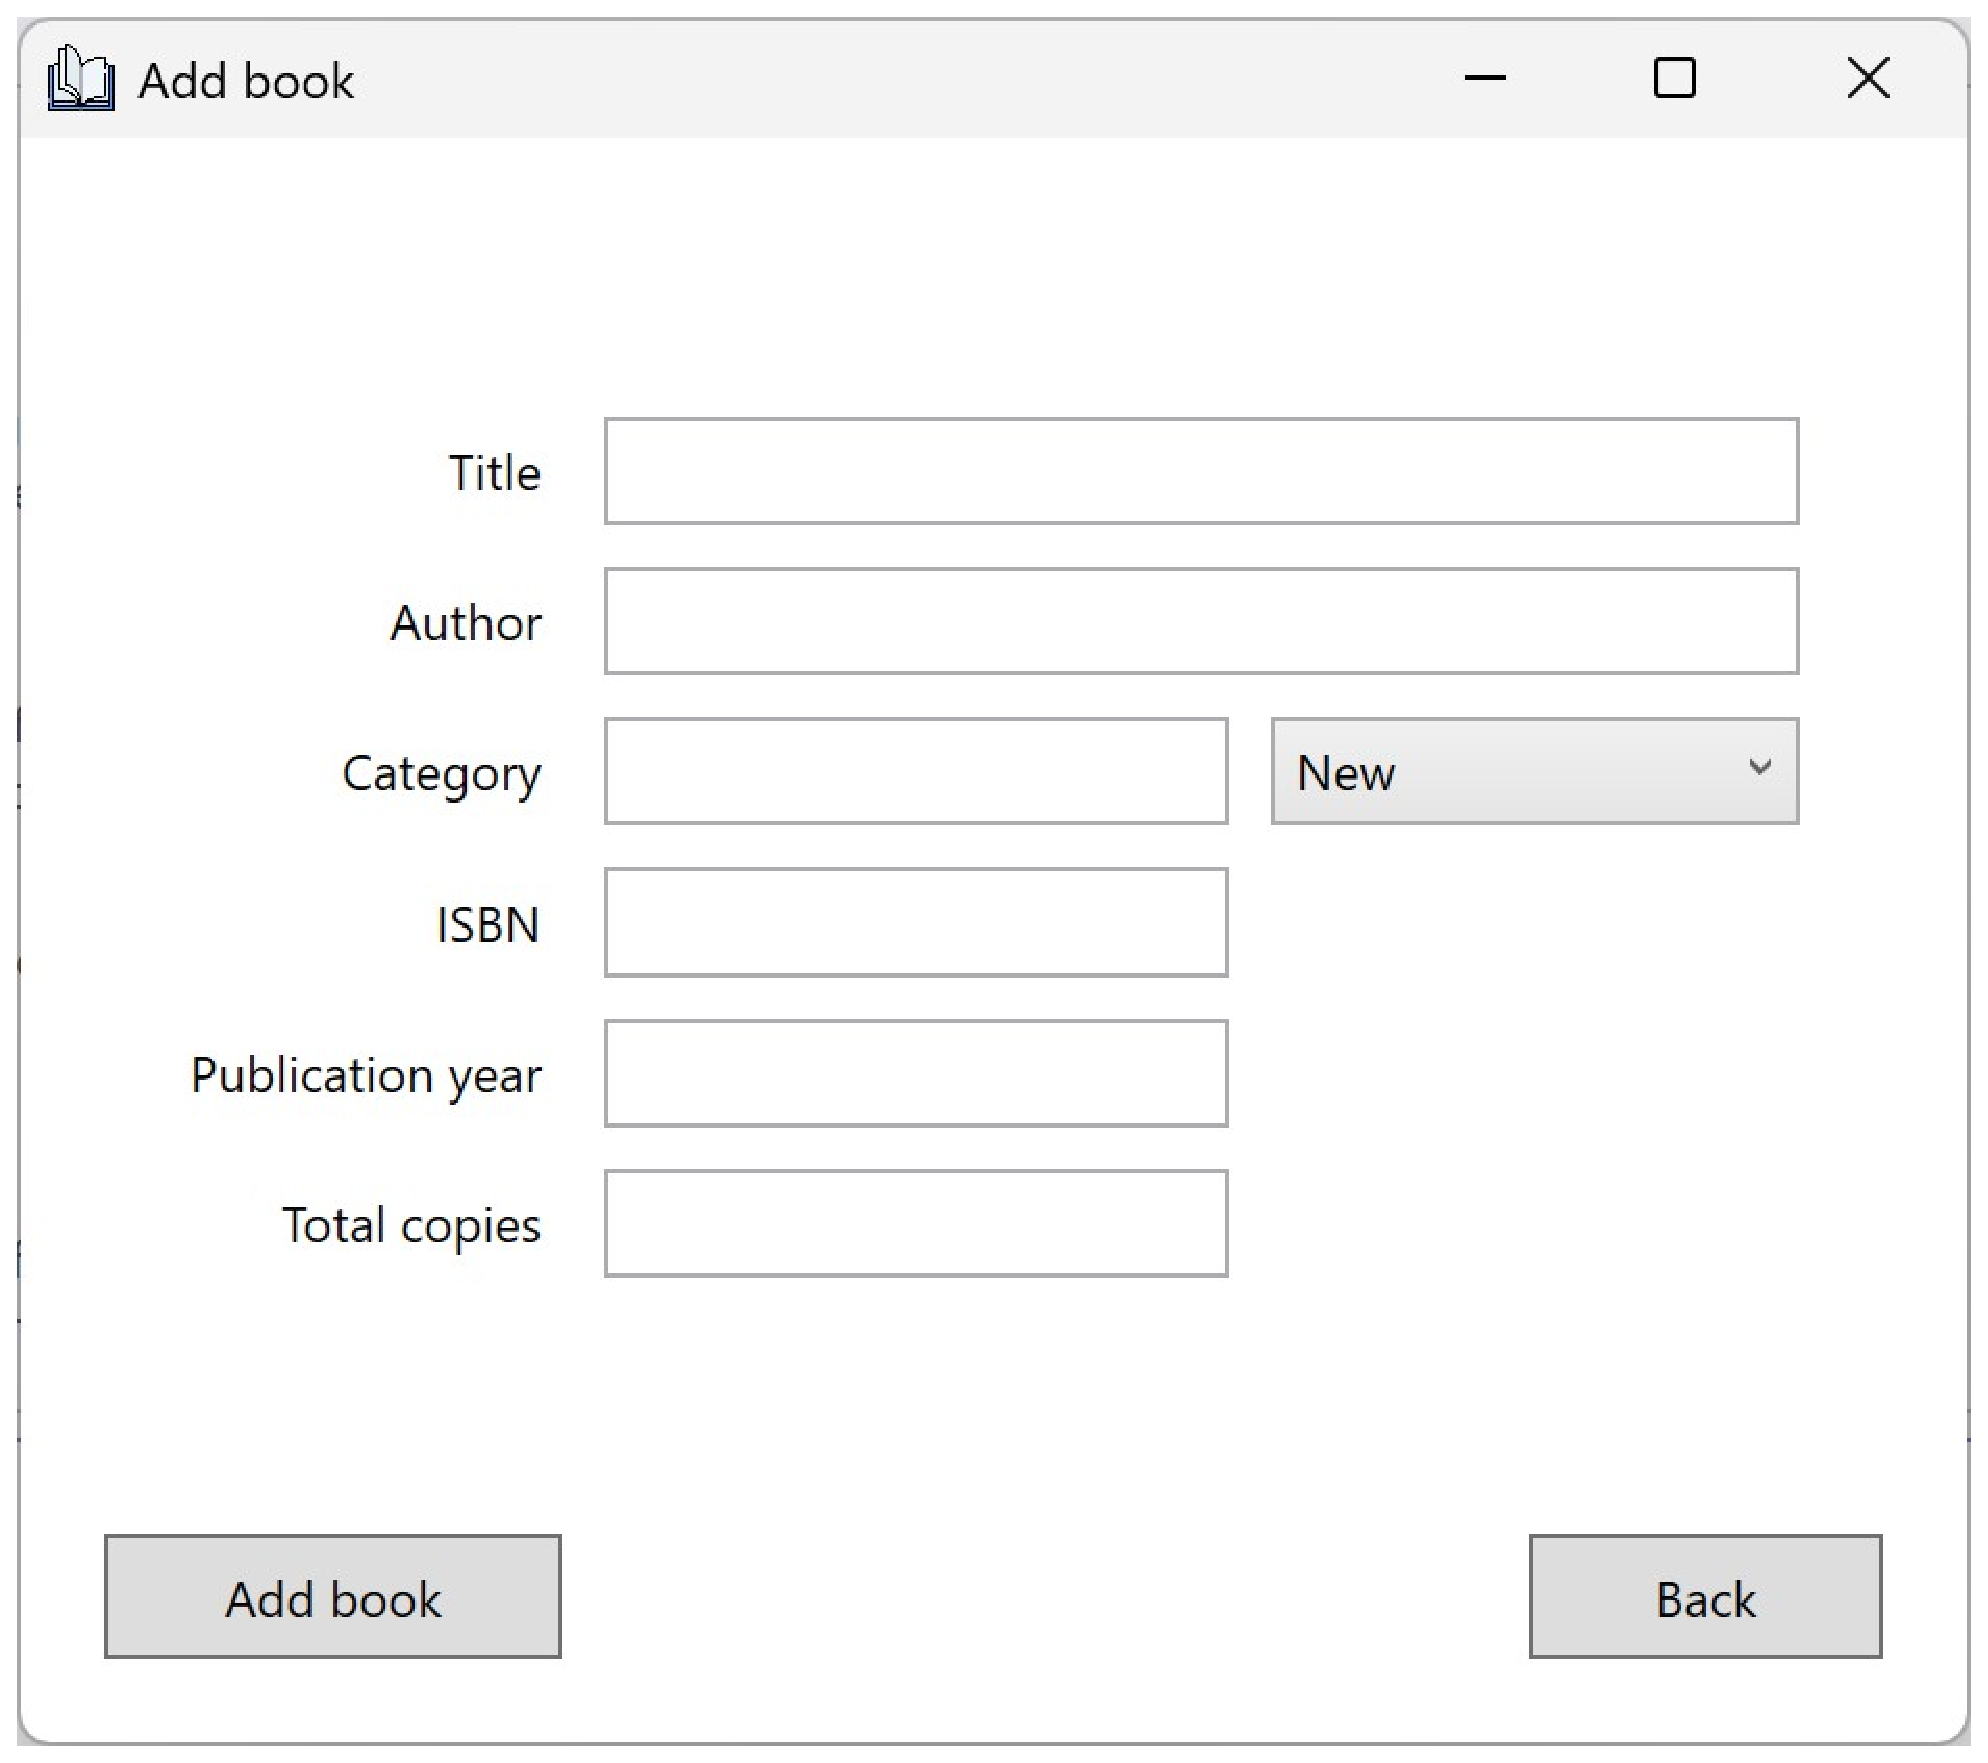
\includegraphics[width=0.6\linewidth]{figures/show/show7.eps}
    \caption{Formularz dodawania nowej książki do bazy.\label{fig:ui_add_book}}
\end{figure}

Modyfikacja metadanych książki odbywa się za pomocą bliźniaczego formularza wywoływanego opcją \textit{Edit book}. Przy uruchomieniu tego okna, wszystkie pola tekstowe są automatycznie uzupełniane danymi wybranej uprzednio z katalogu pozycji. Umożliwia to szybką korektę, na przykład poprawę literówek, przypisanie nowej kategorii, czy aktualizację liczby fizycznych kopii w magazynie.
\begin{figure}[H]
    \centering
    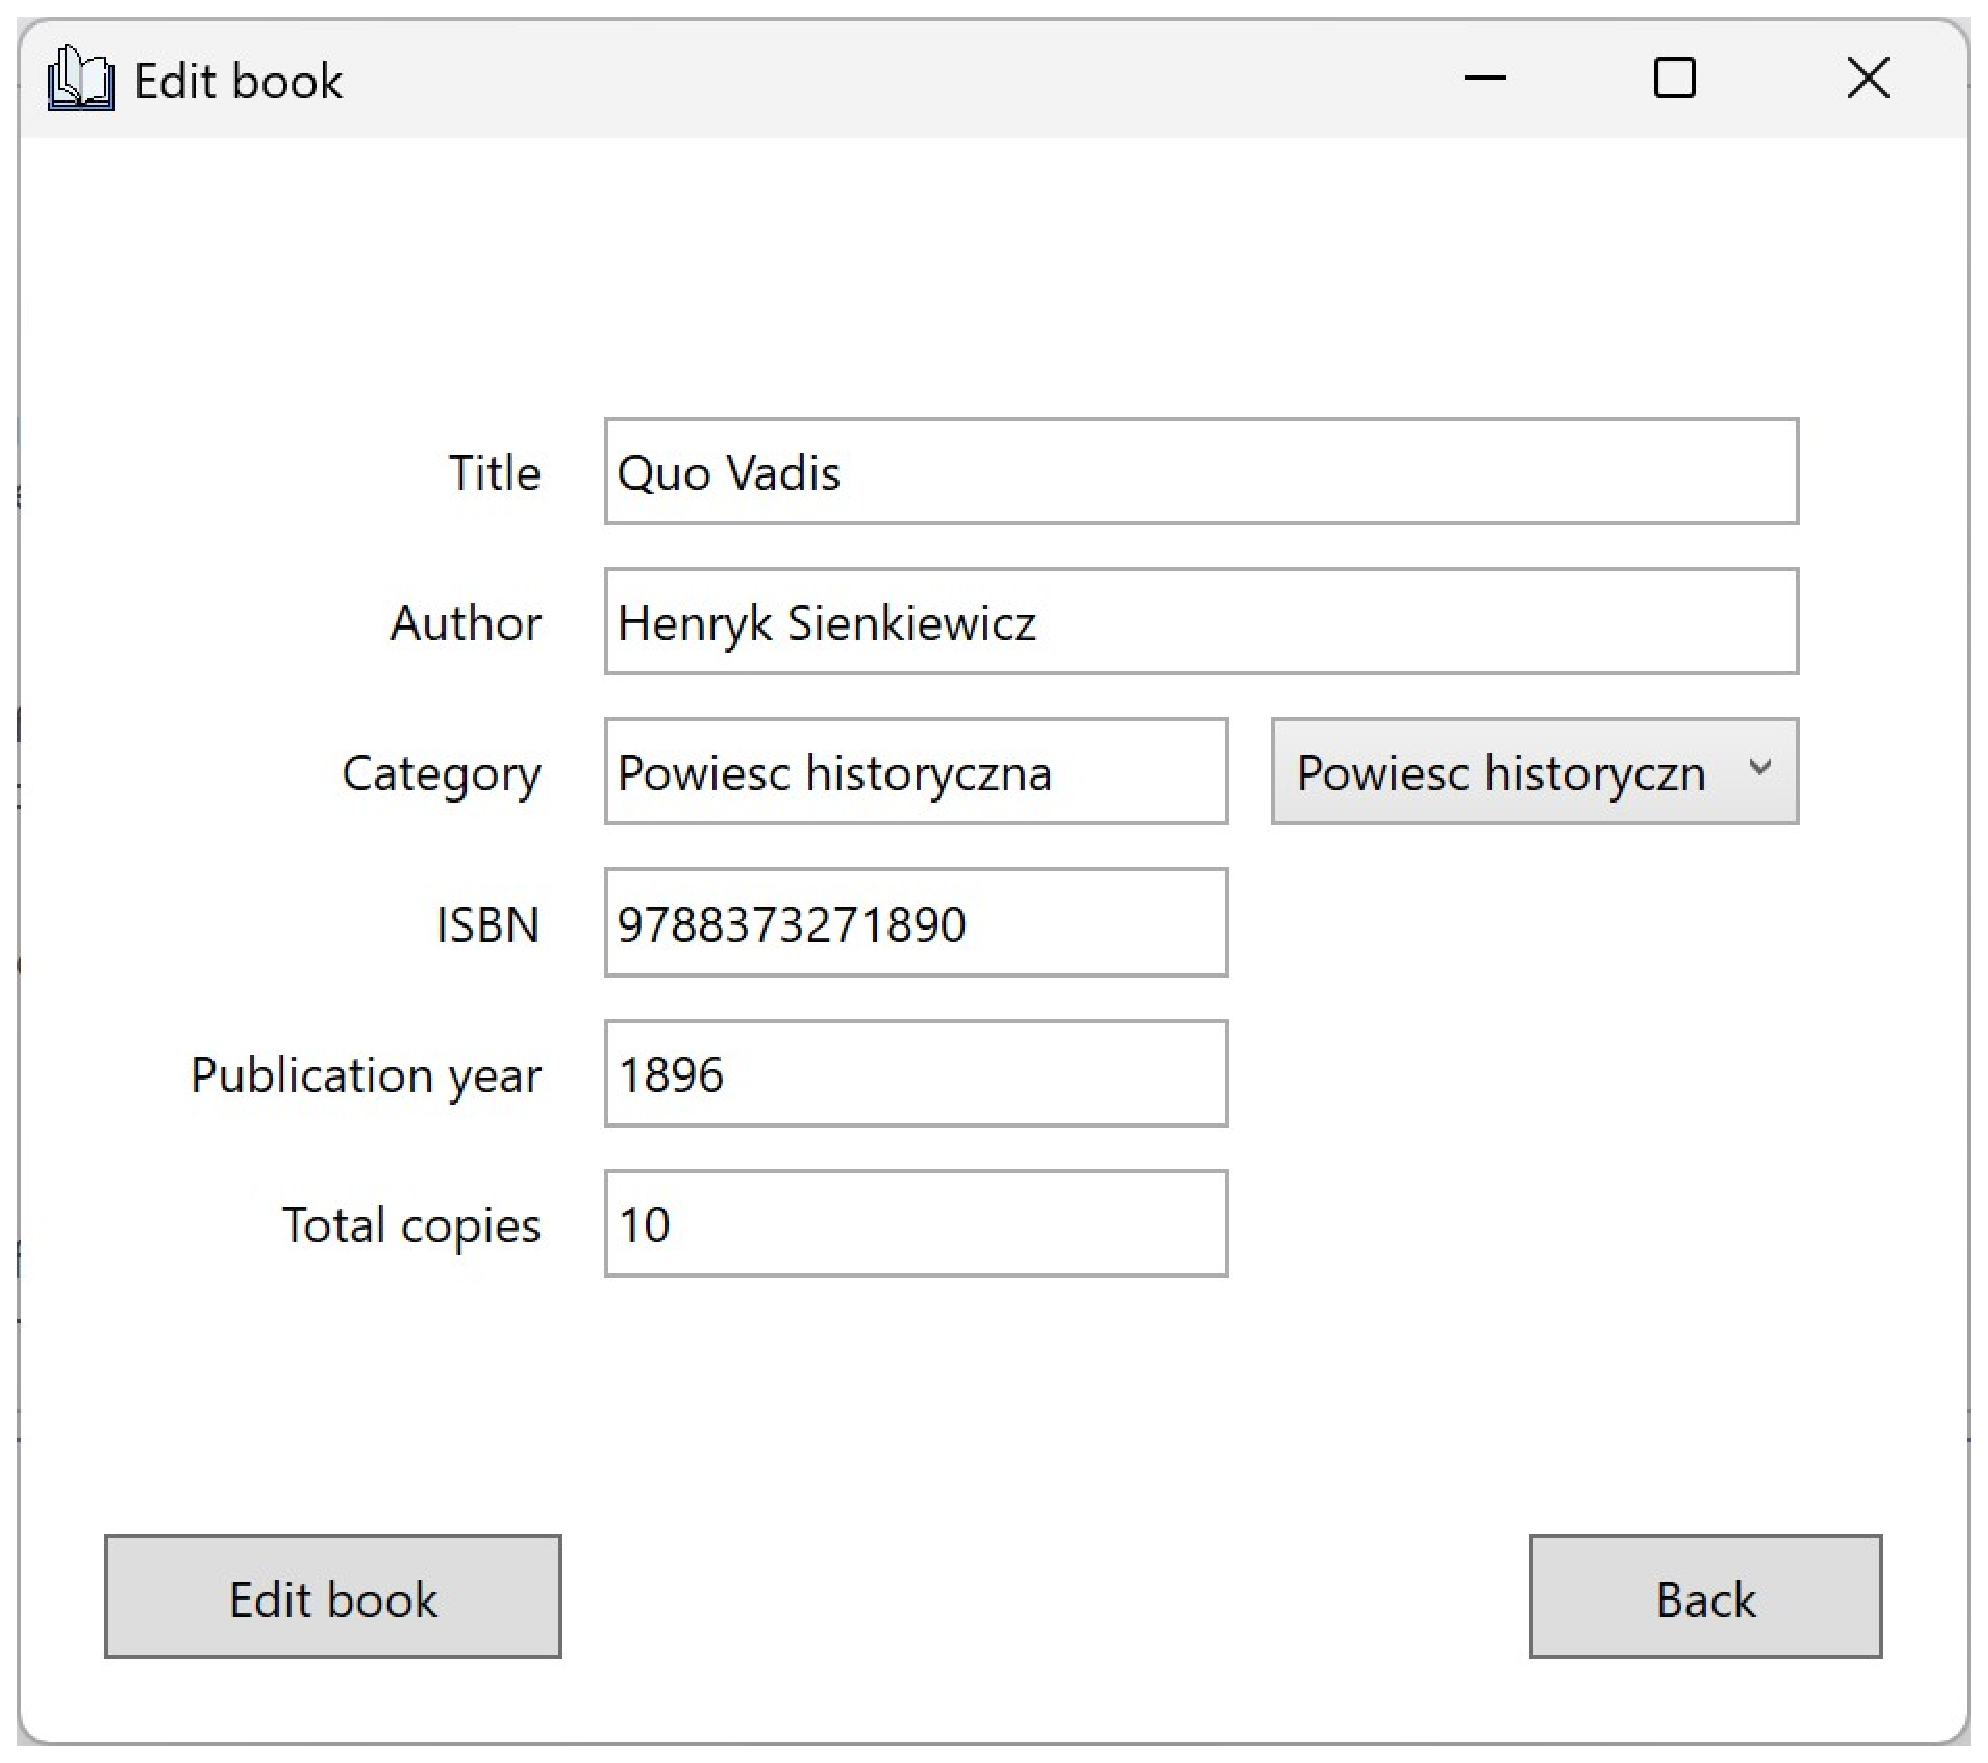
\includegraphics[width=0.6\linewidth]{figures/show/show8.eps}
    \caption{Formularz edycji danych istniejącej książki.\label{fig:ui_edit_book}}
\end{figure}

Bibliotekarz ma dostęp do listy wszystkich zarejestrowanych użytkowników (\textit{View user list}). Widok ten udostępnia tabelę z danymi kont (Id, nazwisko, imię, nazwa użytkownika, rola) oraz wyszukiwarkę pozwalającą filtrować użytkowników po imieniu, nazwisku lub loginie, a także według roli (\textit{Reader}/\textit{Librarian}). Dostępne przyciski pozwalają na podgląd szczegółów, edycję, dodanie nowego konta oraz usunięcie wybranego użytkownika.
\begin{figure}[H]
    \centering
    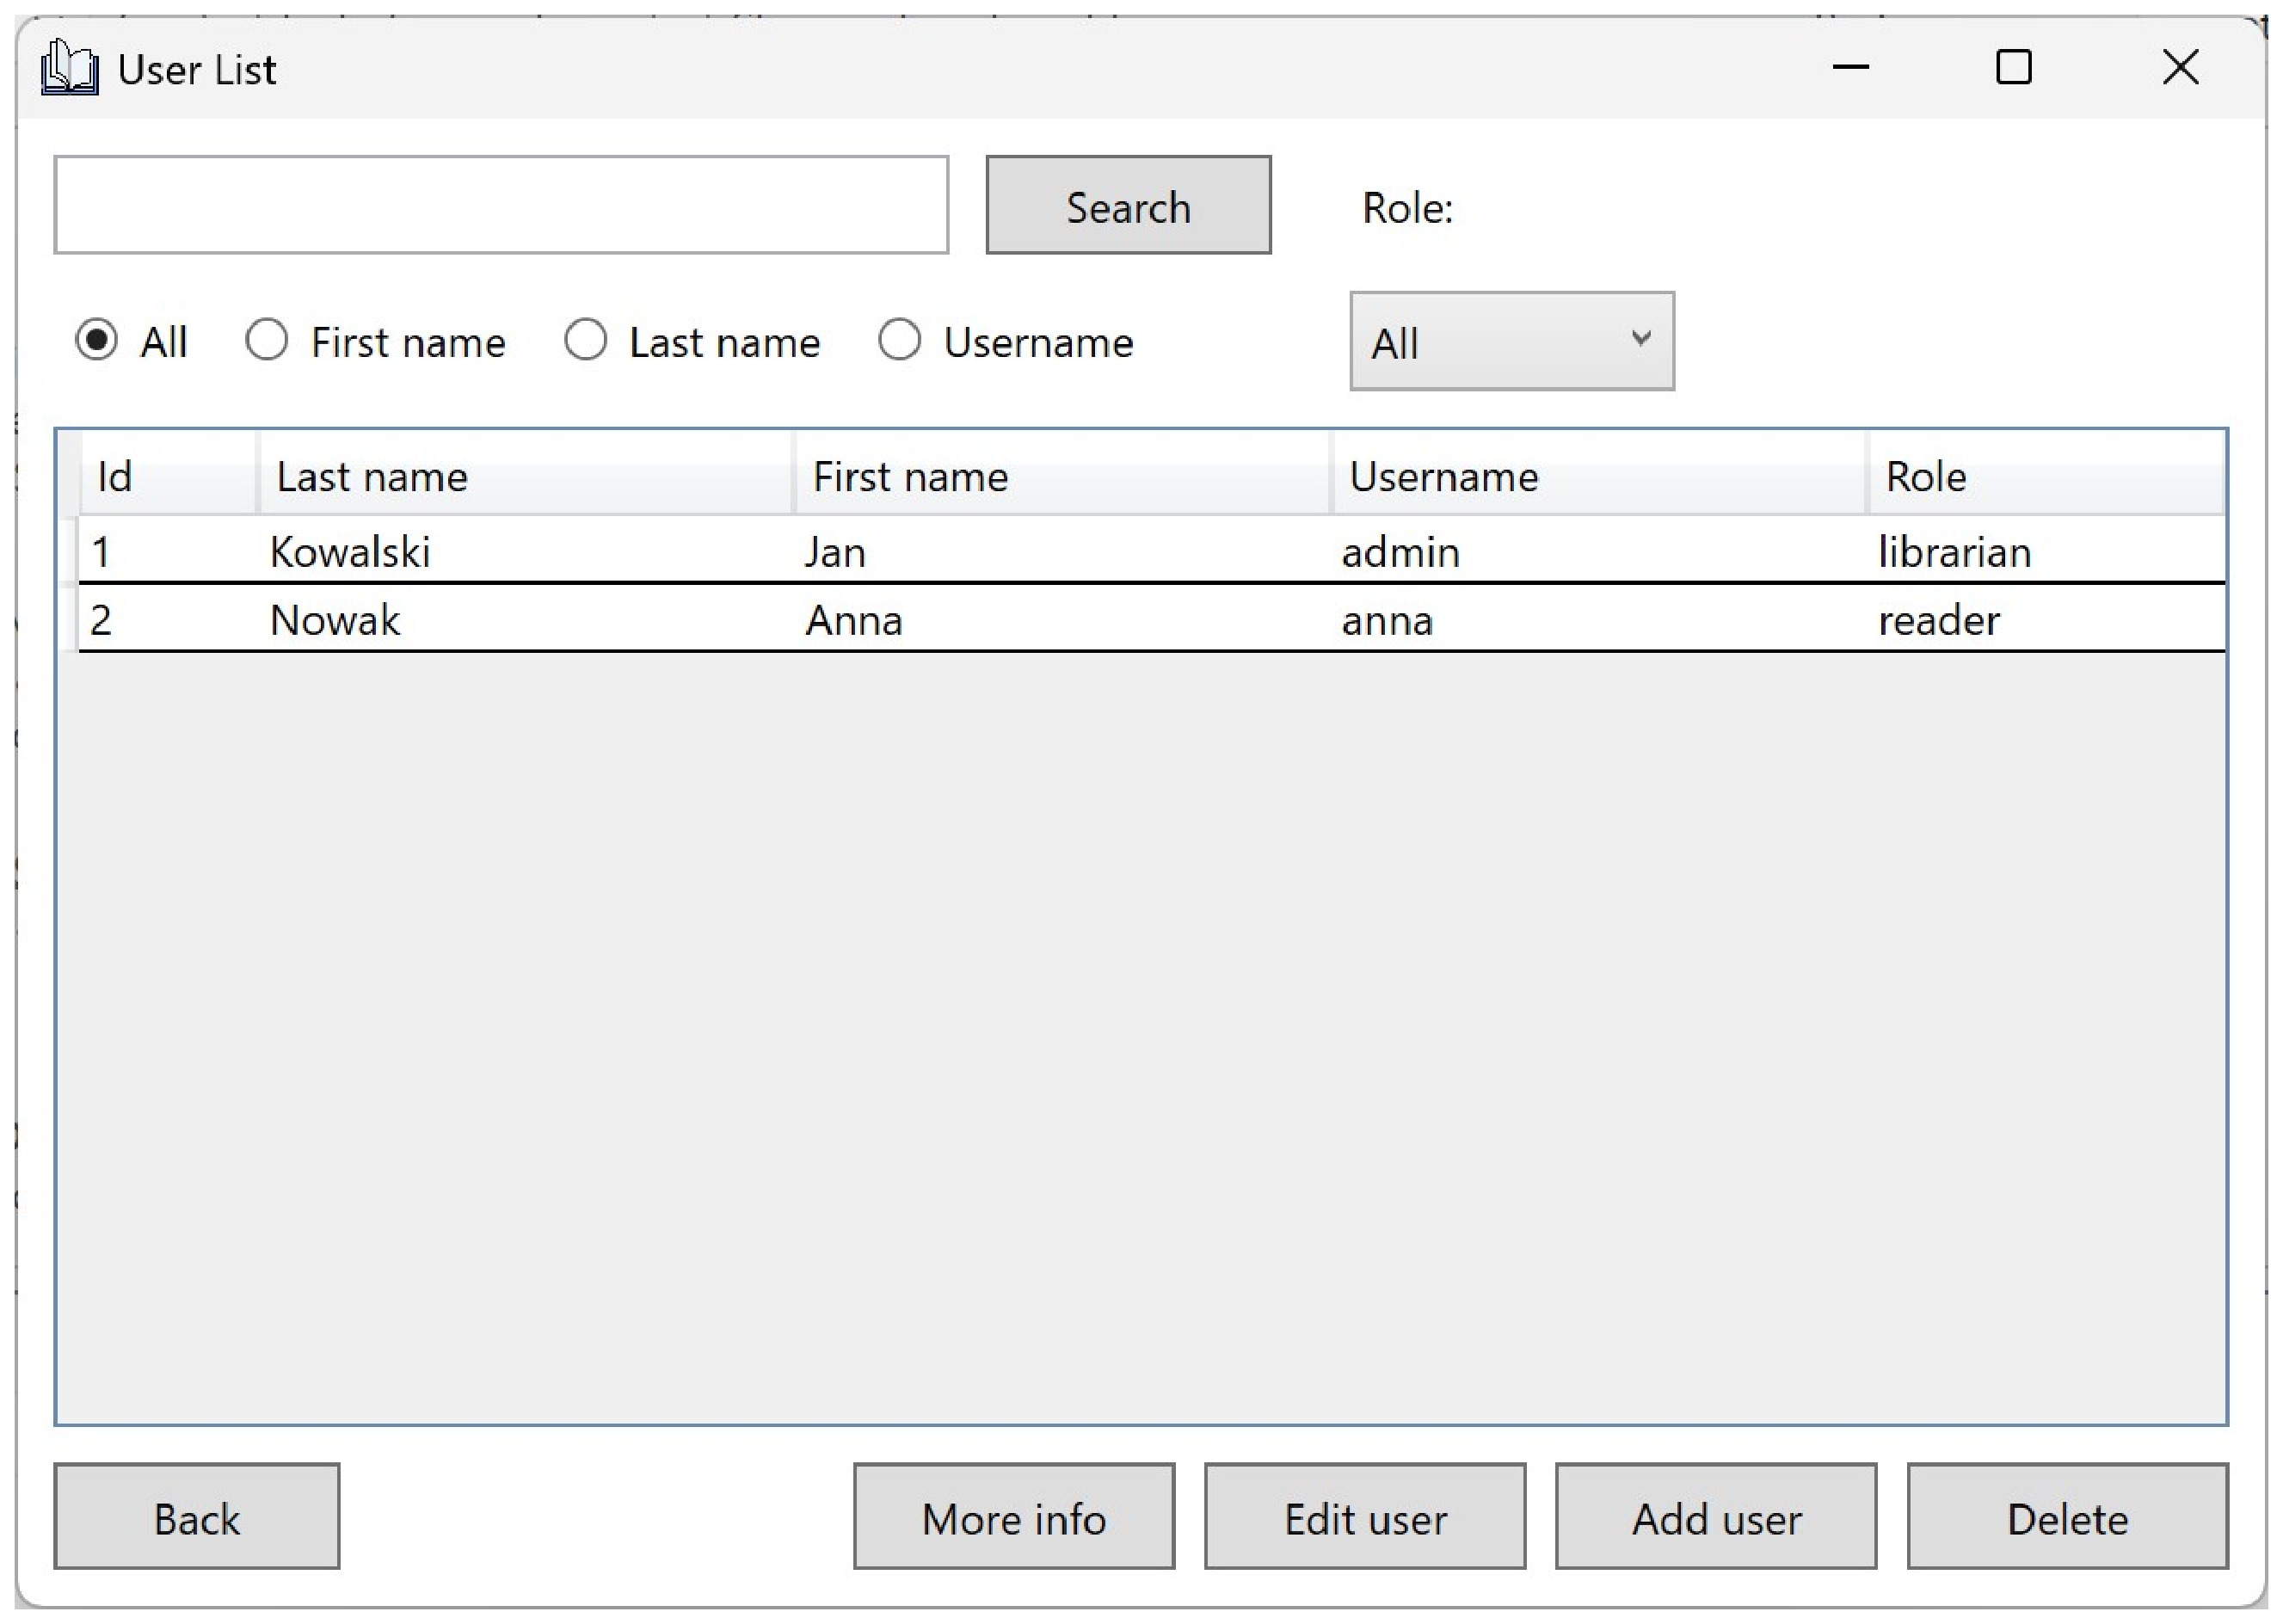
\includegraphics[width=0.8\linewidth]{figures/show/show9.eps}
    \caption{Lista użytkowników z opcjami zarządzania kontami.\label{fig:ui_user_list}}
\end{figure}

Formularz edycji użytkownika, dostępny po wybraniu konta z listy i kliknięciu \textit{Edit user}, wczytuje automatycznie aktualne dane wybranej osoby. Bibliotekarz może zmodyfikować imię, nazwisko, nazwę użytkownika oraz zmienić przypisaną rolę za pomocą rozwijanej listy.
\begin{figure}[H]
    \centering
    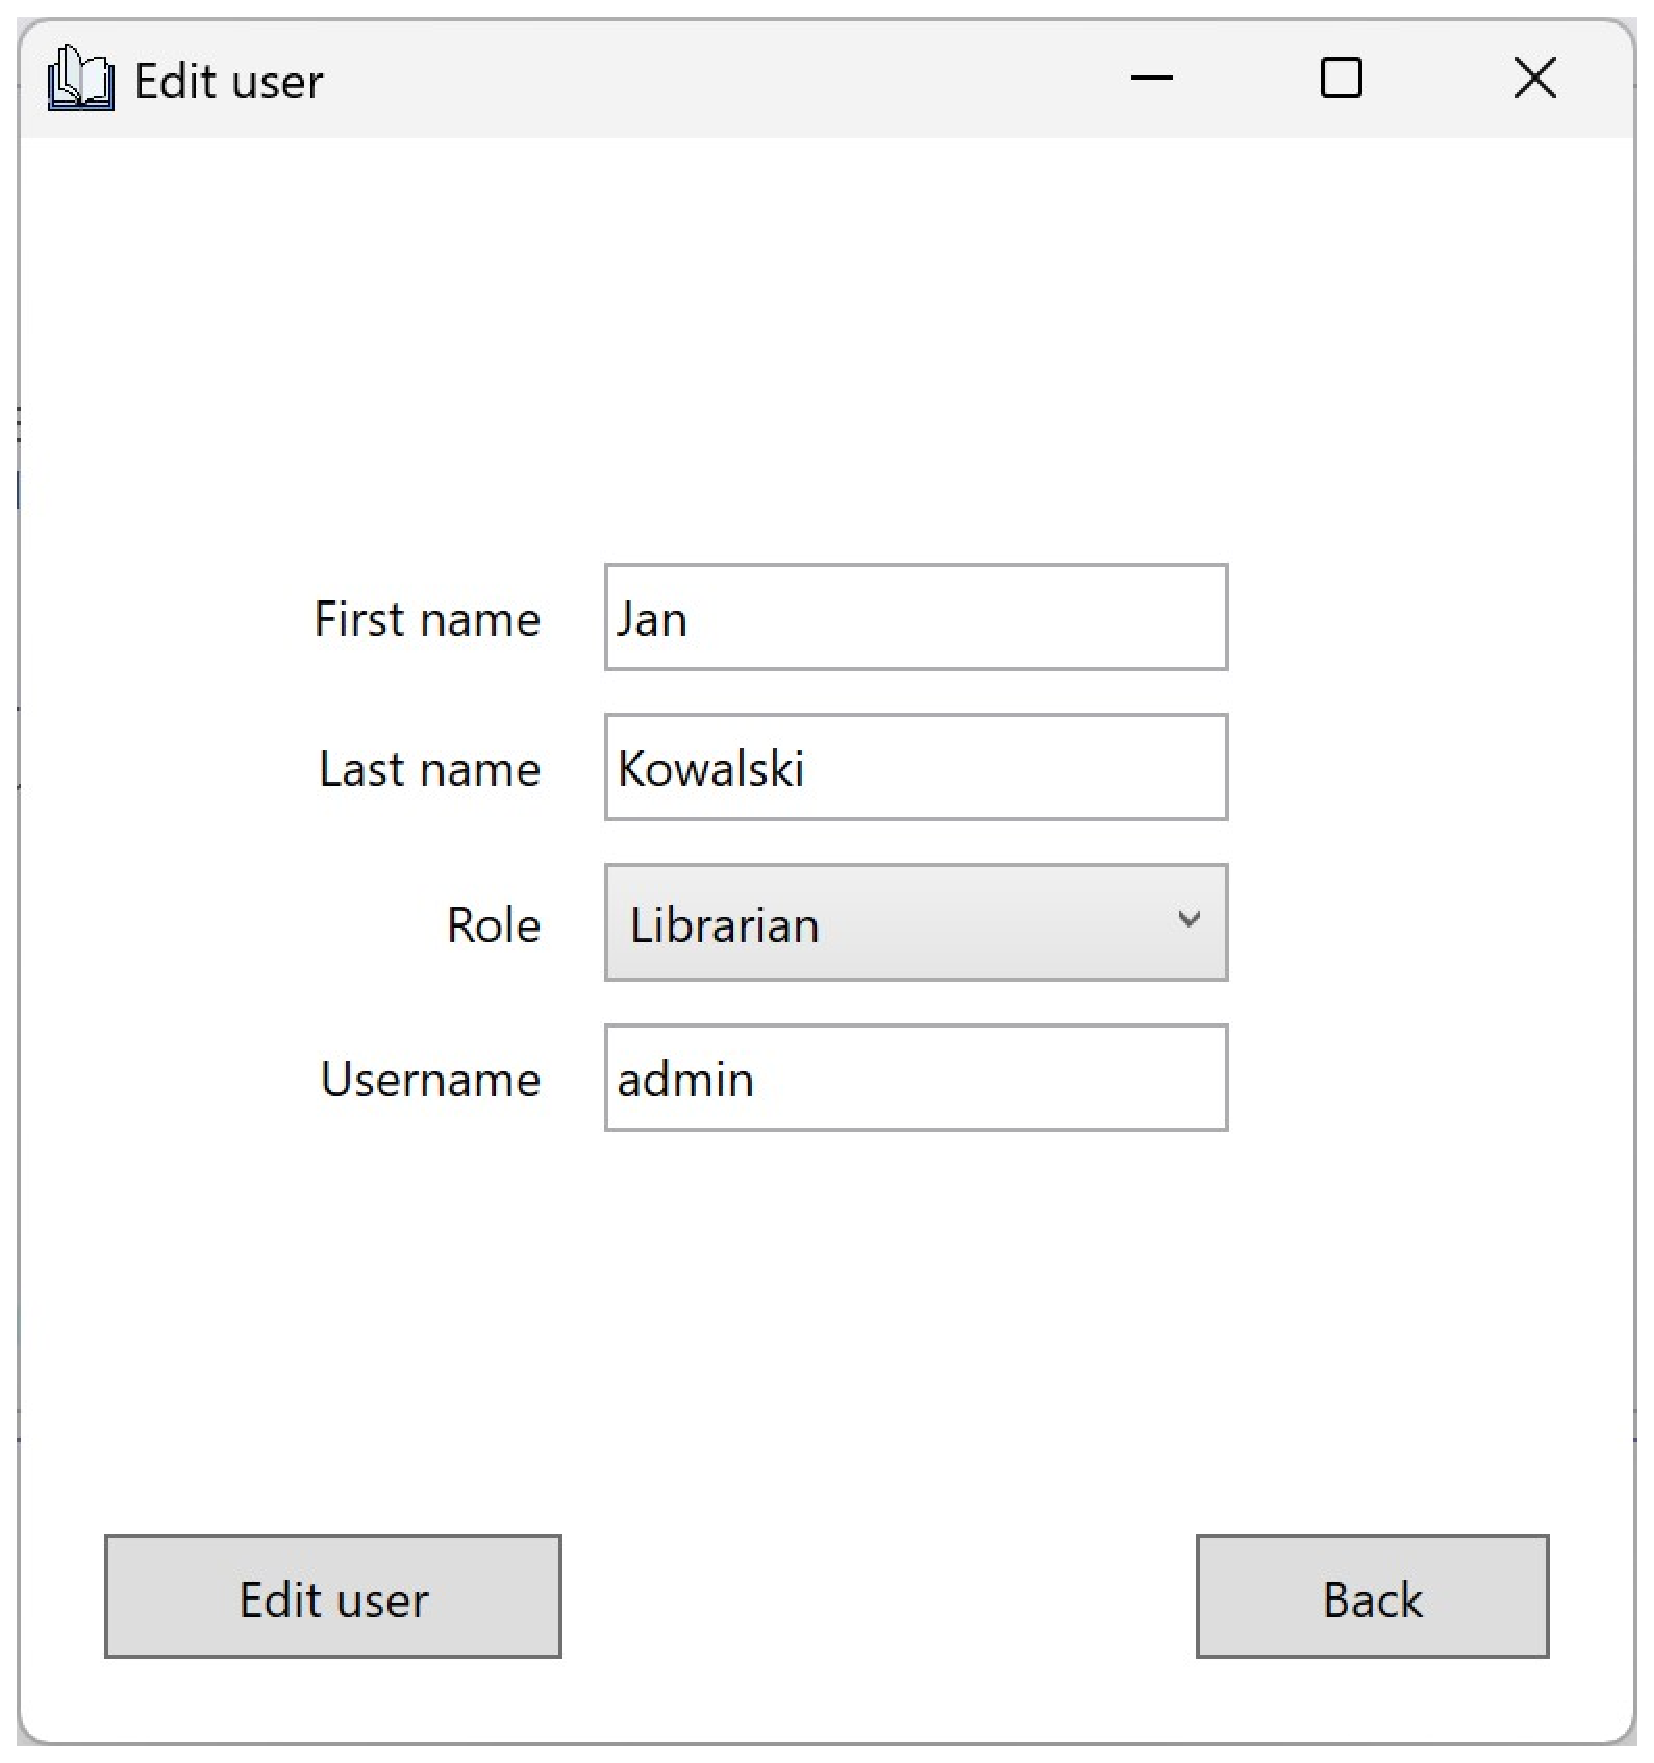
\includegraphics[width=0.6\linewidth]{figures/show/show11.eps}
    \caption{Formularz edycji danych użytkownika.\label{fig:ui_edit_user}}
\end{figure}

Opcja \textit{Add user} otwiera formularz tworzenia nowego konta z poziomu panelu administratora. W odróżnieniu od rejestracji dostępnej dla niezalogowanych, ten widok pozwala bibliotekarzowi bezpośrednio przypisać rolę tworzonemu kontu (Reader lub Librarian). Formularz wymaga uzupełnienia imienia, nazwiska, nazwy użytkownika, hasła i potwierdzenia hasła.
\begin{figure}[H]
    \centering
    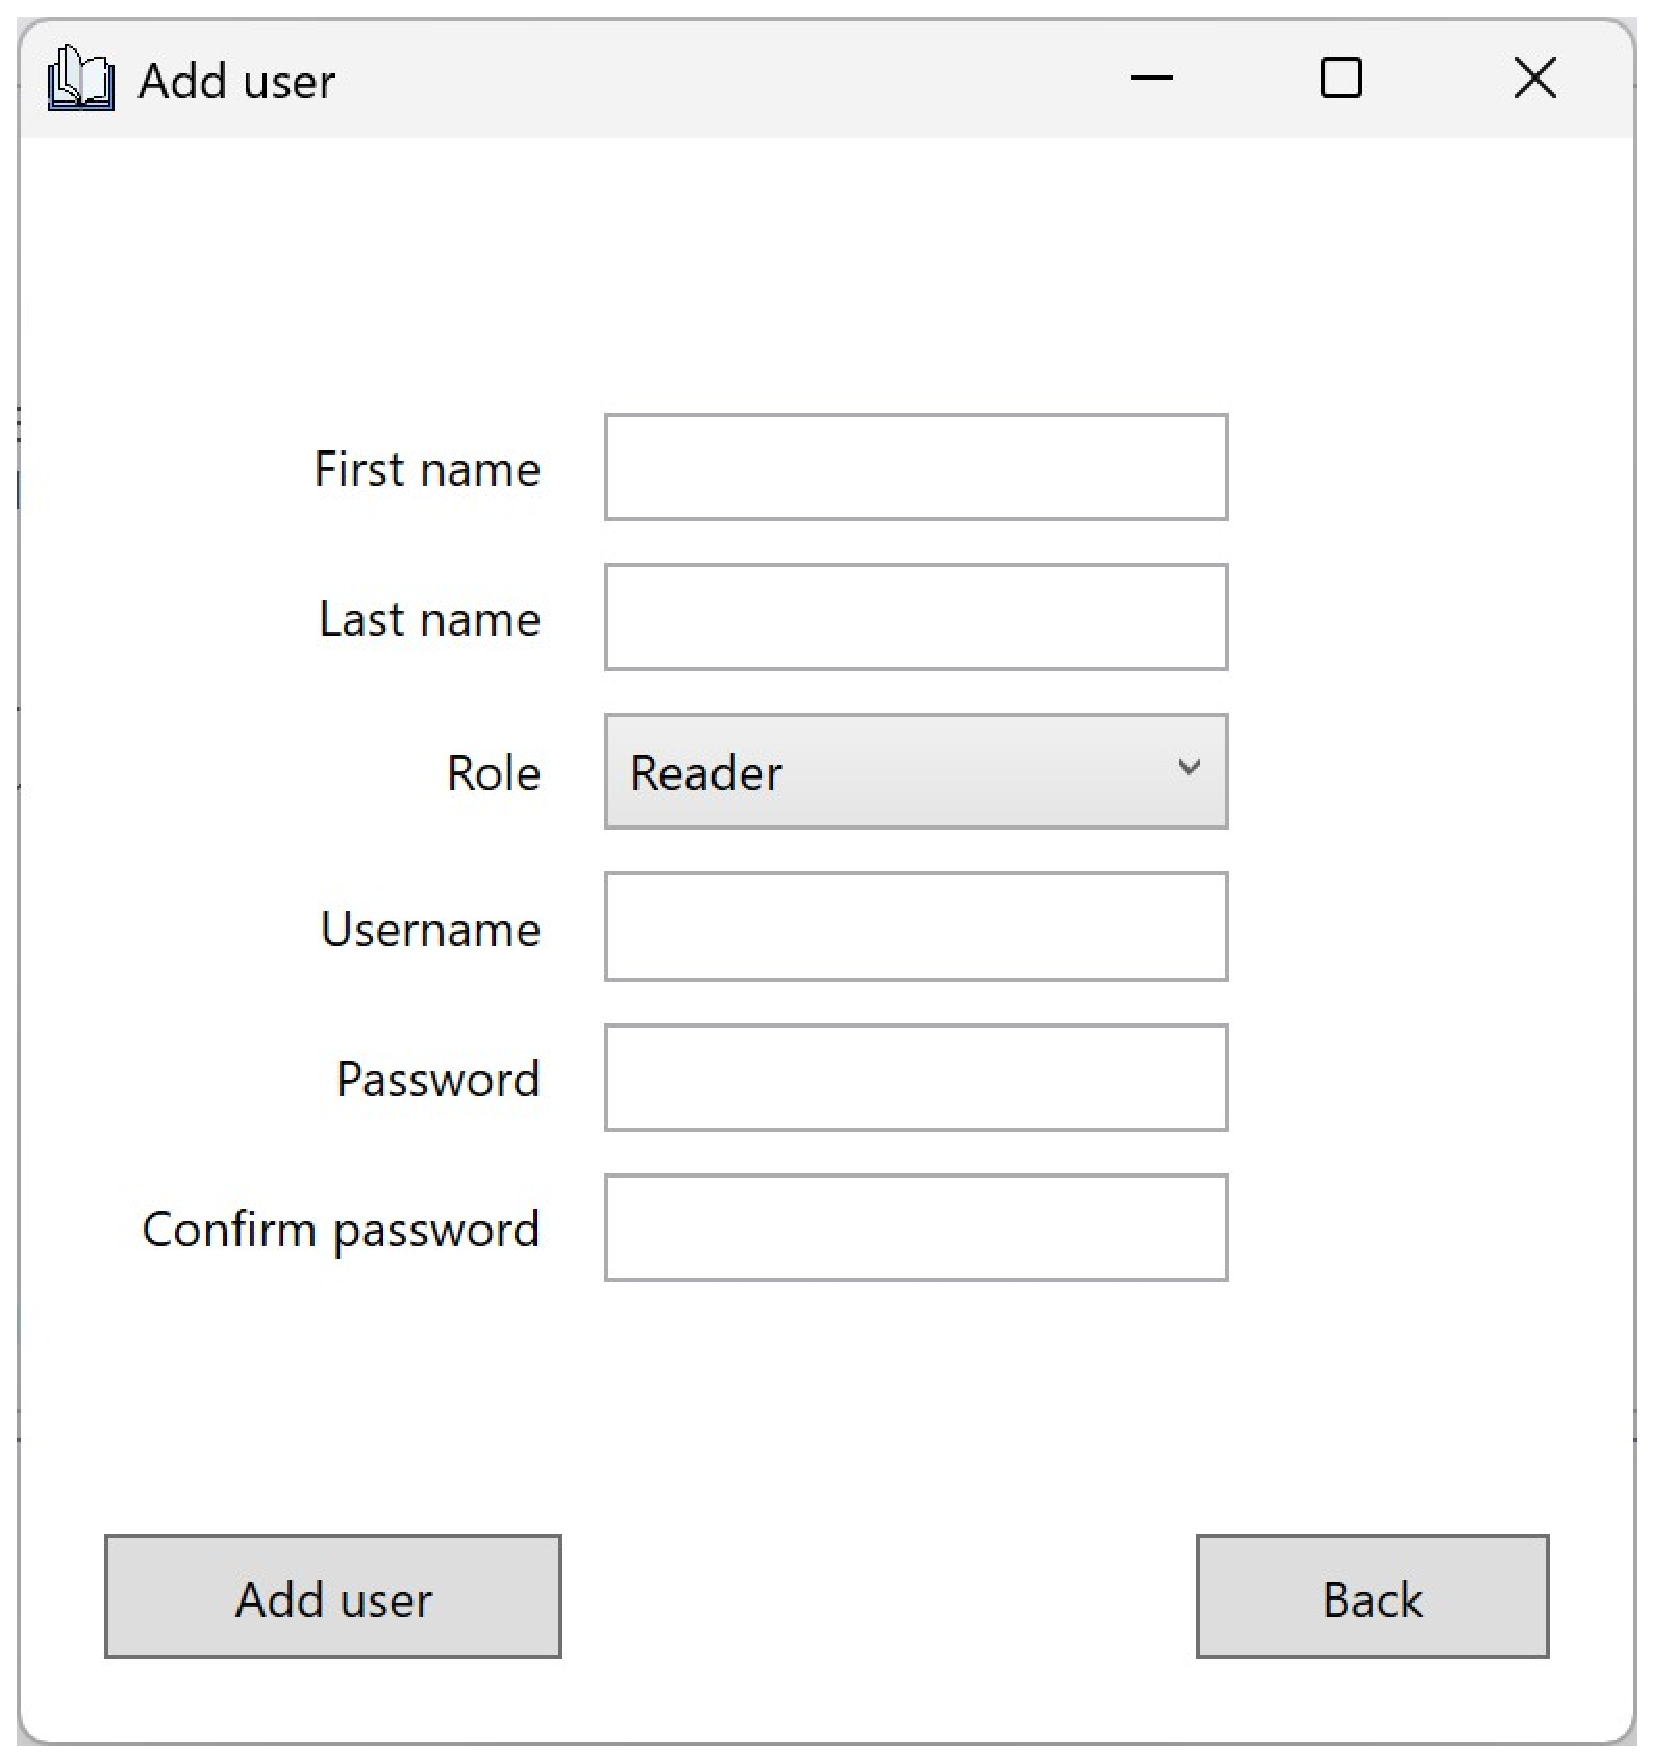
\includegraphics[width=0.6\linewidth]{figures/show/show10.eps}
    \caption{Formularz dodawania nowego użytkownika przez bibliotekarza.\label{fig:ui_add_user}}
\end{figure}

Obsługa zwrotów odbywa się przez dedykowany widok \textit{Return Book}. Bibliotekarz widzi tabelę aktywnych wypożyczeń zawierającą wszystkie istotne informacje: dane książki (tytuł, autor, ISBN), daty (data wypożyczenia oraz termin zwrotu), a po dokonaniu zwrotu -- datę oddania i ewentualnie naliczoną kwotę kary za opóźnienie (w PLN). Zaznaczenie rekordu i kliknięcie \textit{Return Book} finalizuje operację w systemie.
\begin{figure}[H]
    \centering
    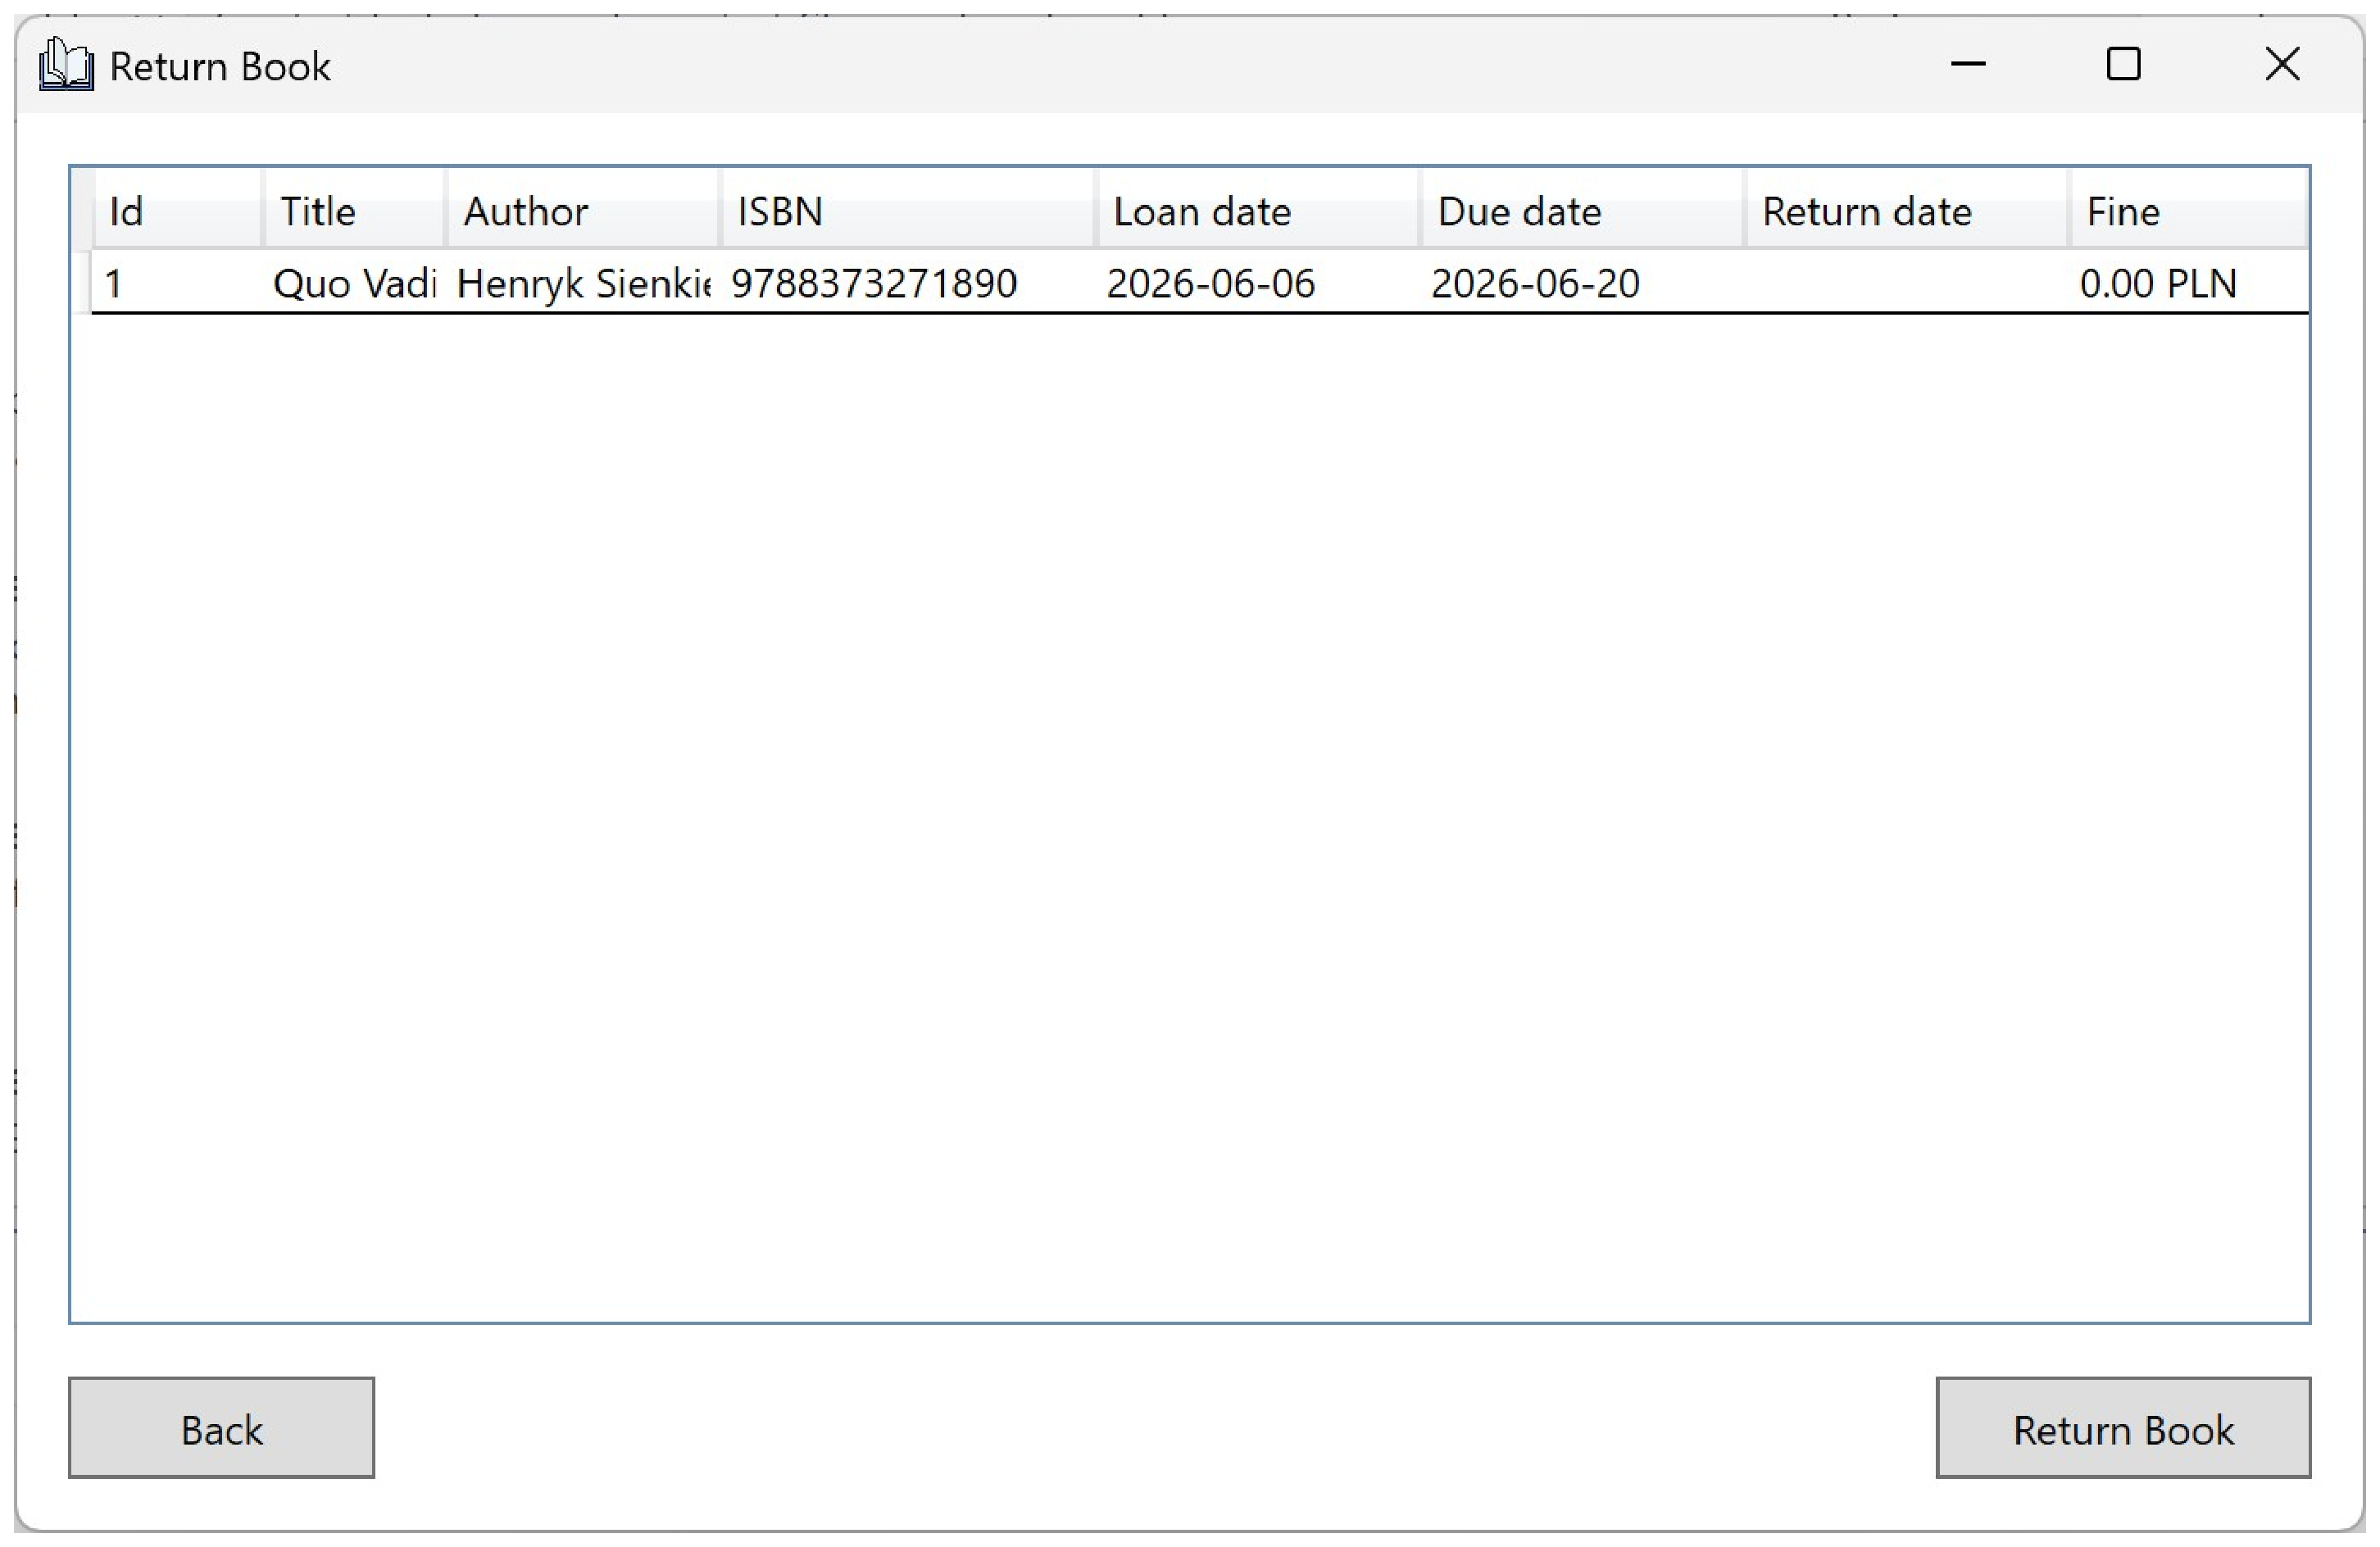
\includegraphics[width=0.8\linewidth]{figures/show/show12.eps}
    \caption{Panel obsługi zwrotów wypożyczonych książek.\label{fig:ui_return_book}}
\end{figure}

Każdy zalogowany użytkownik (zarówno czytelnik jak i bibliotekarz) ma możliwość zmiany swojego hasła dostępową poprzez opcję \textit{Change password} w menu głównym. Formularz wymaga podania nowego hasła oraz jego potwierdzenia w celu wyeliminowania pomyłki.
\begin{figure}[H]
    \centering
    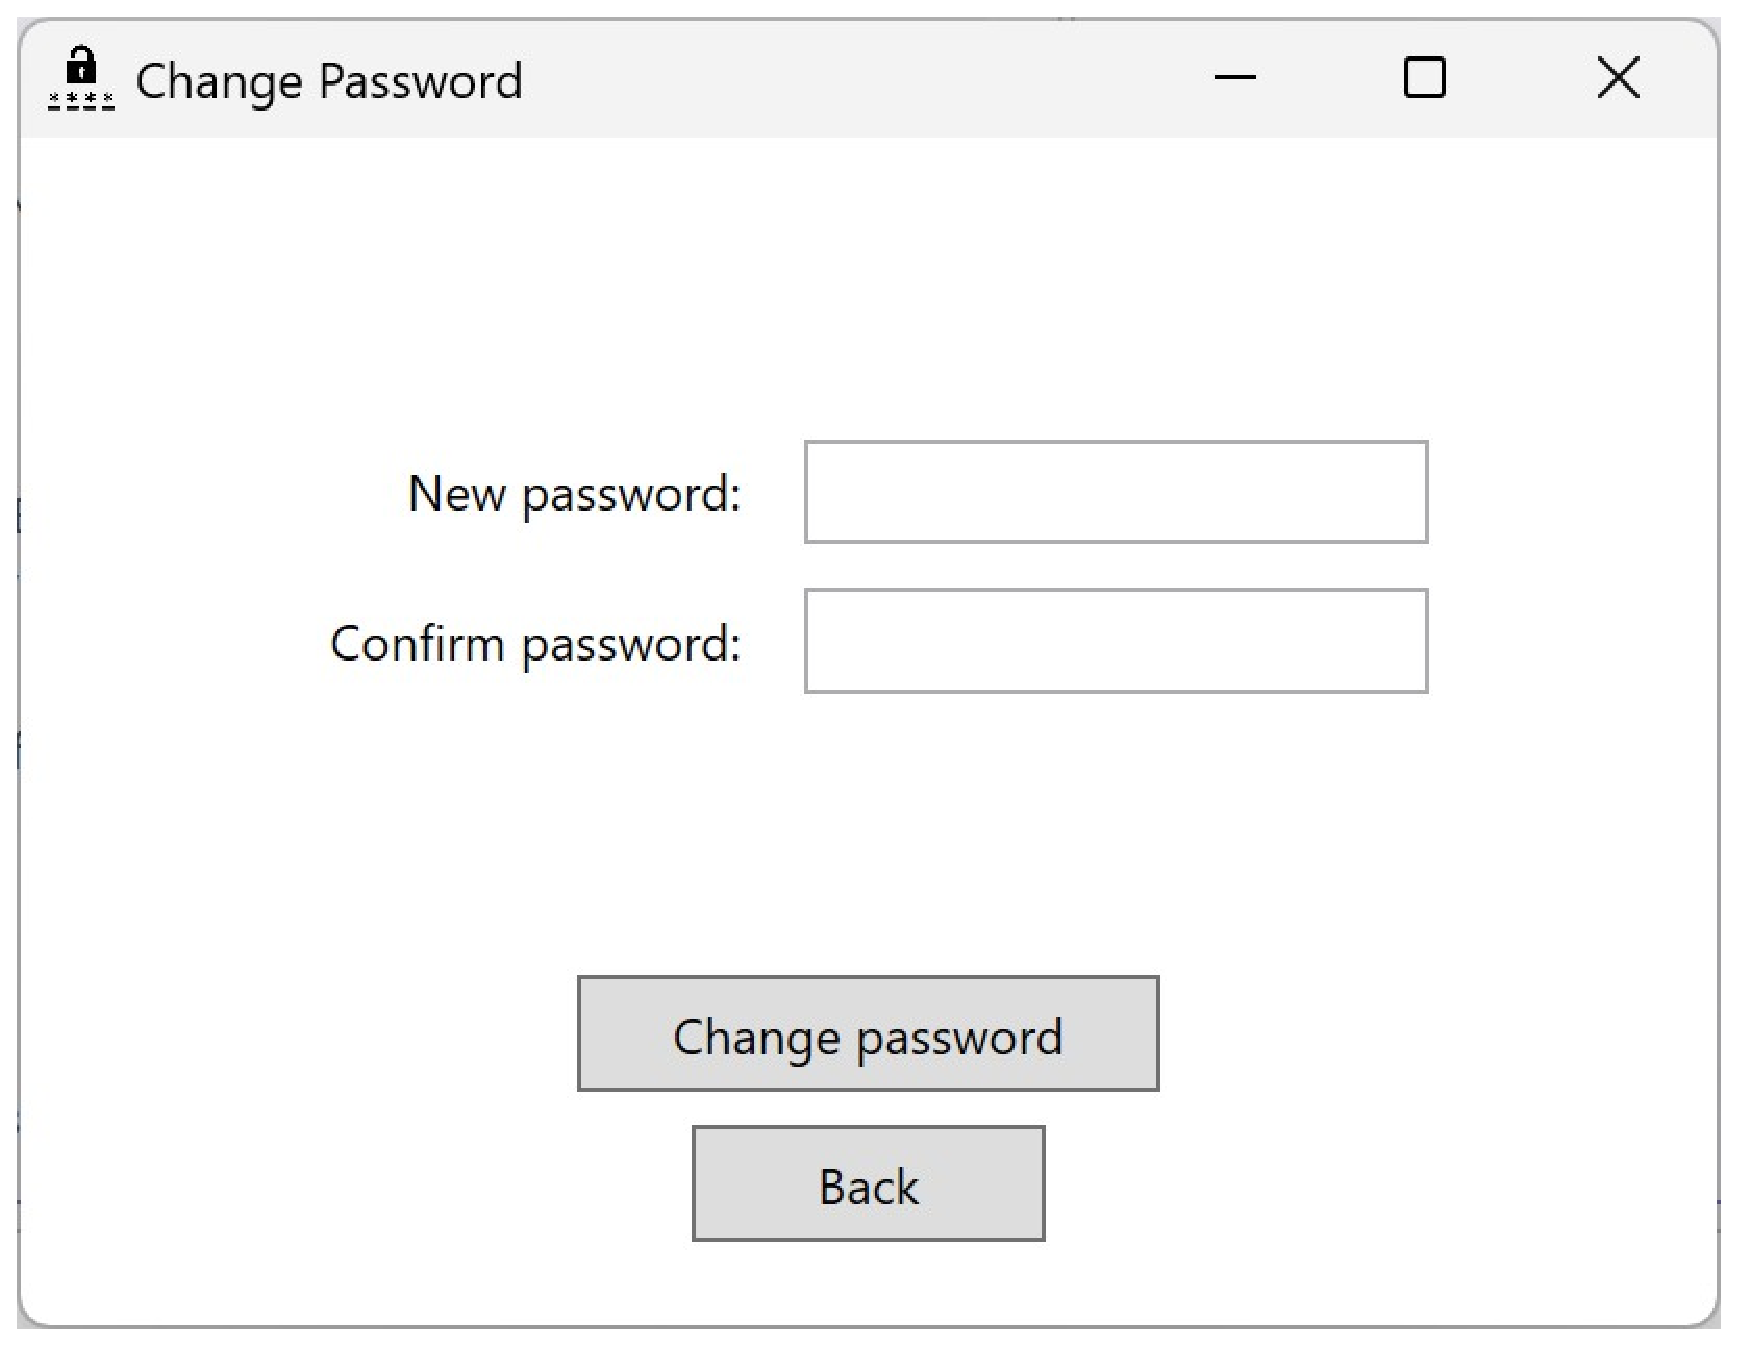
\includegraphics[width=0.55\linewidth]{figures/show/show14.eps}
    \caption{Formularz zmiany hasła użytkownika.\label{fig:ui_change_password}}
\end{figure}

Wyszukiwarka na liście użytkowników działa dynamicznie -- poniższy przykład ilustruje filtrowanie po imieniu (pole \textit{First name}) z wpisaną frazą ,,A''. System wyświetla wyłącznie pasujące rekordy, w tym przypadku użytkowniczkę Annę Nowak z rolą \textit{reader}.
\begin{figure}[H]
    \centering
    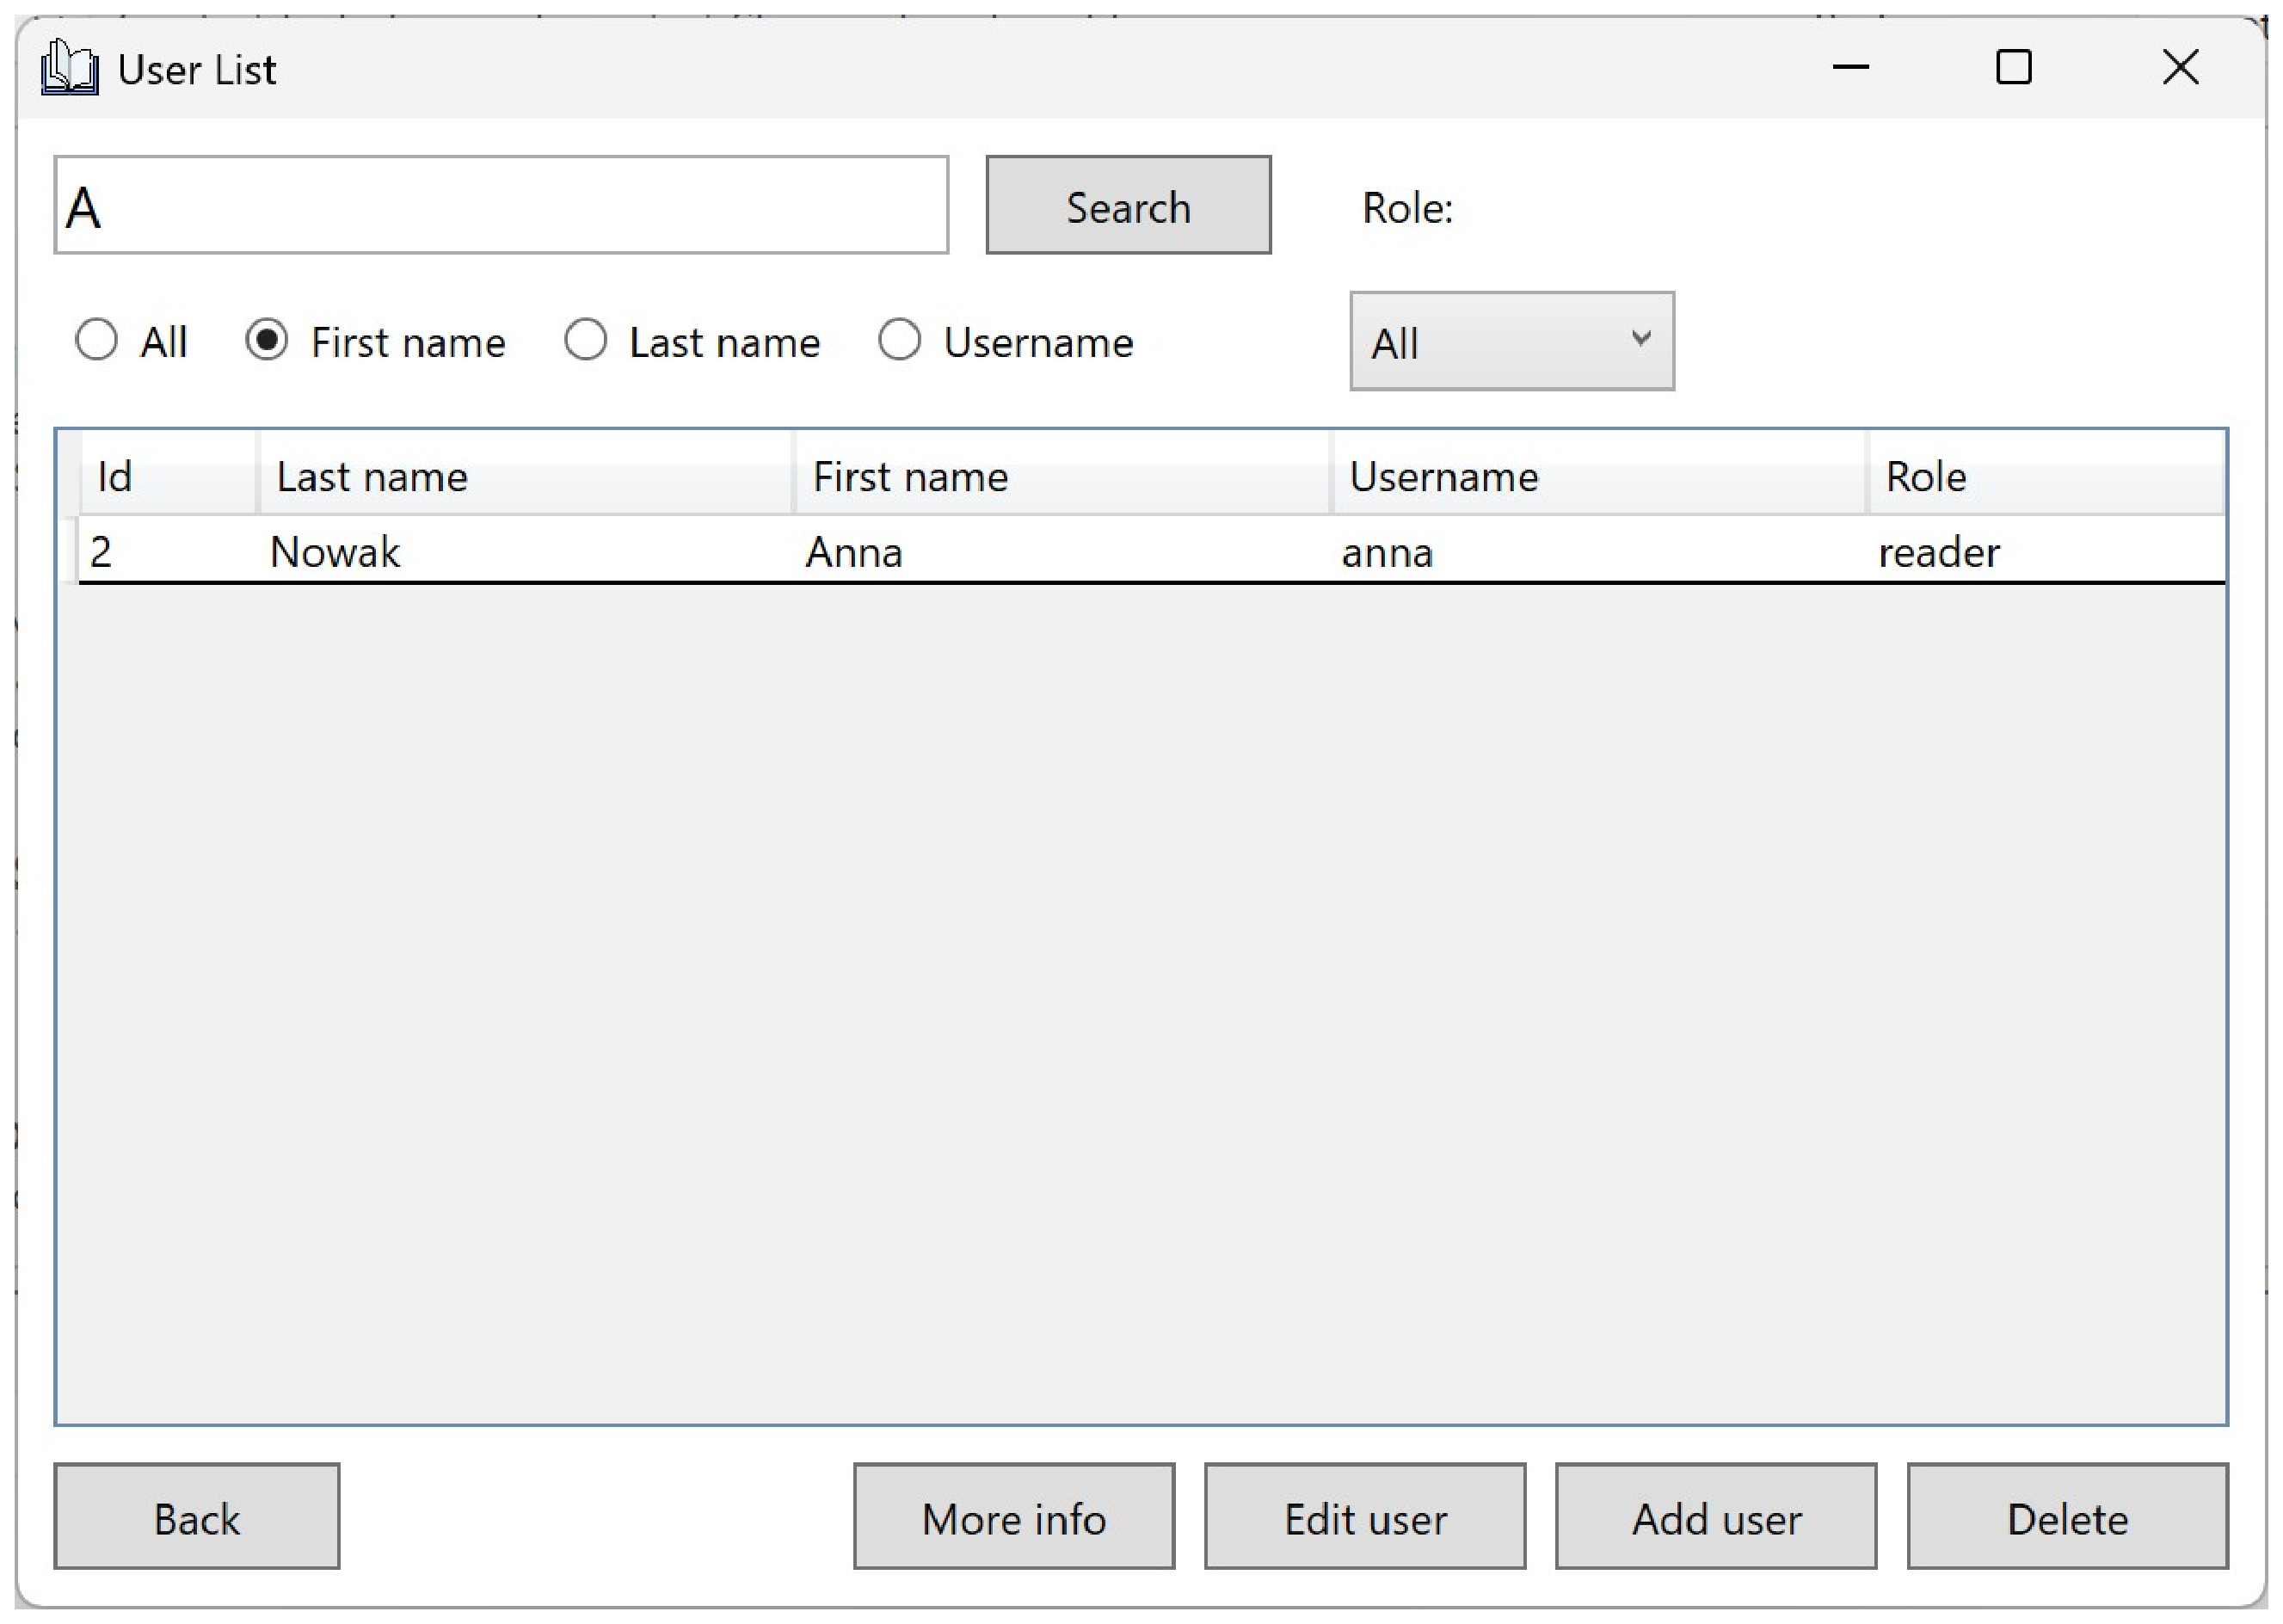
\includegraphics[width=0.8\linewidth]{figures/show/show13.eps}
    \caption{Przykład działania wyszukiwarki na liście użytkowników.\label{fig:ui_user_search}}
\end{figure}

Format pliku eksportu danych to \textbf{JSON} (\texttt{LibraryBackup.json}). Plik zawiera ustrukturyzowane dane wszystkich wybranych tabel w postaci zagnieżdżonych obiektów. Każdy rekord użytkownika zawiera m.in. pola: \texttt{IdUser}, \texttt{Username}, \texttt{Password} (w postaci zahashowanej, co gwarantuje bezpieczeństwo danych), \texttt{FirstName}, \texttt{LastName}, \texttt{Role} oraz zagnieżdżony obiekt \texttt{UserRole} z listą powiązanych encji. Plik ten może zostać ponownie zaimportowany do systemu poprzez mechanizm \textit{Import data}.
\begin{figure}[H]
    \centering
    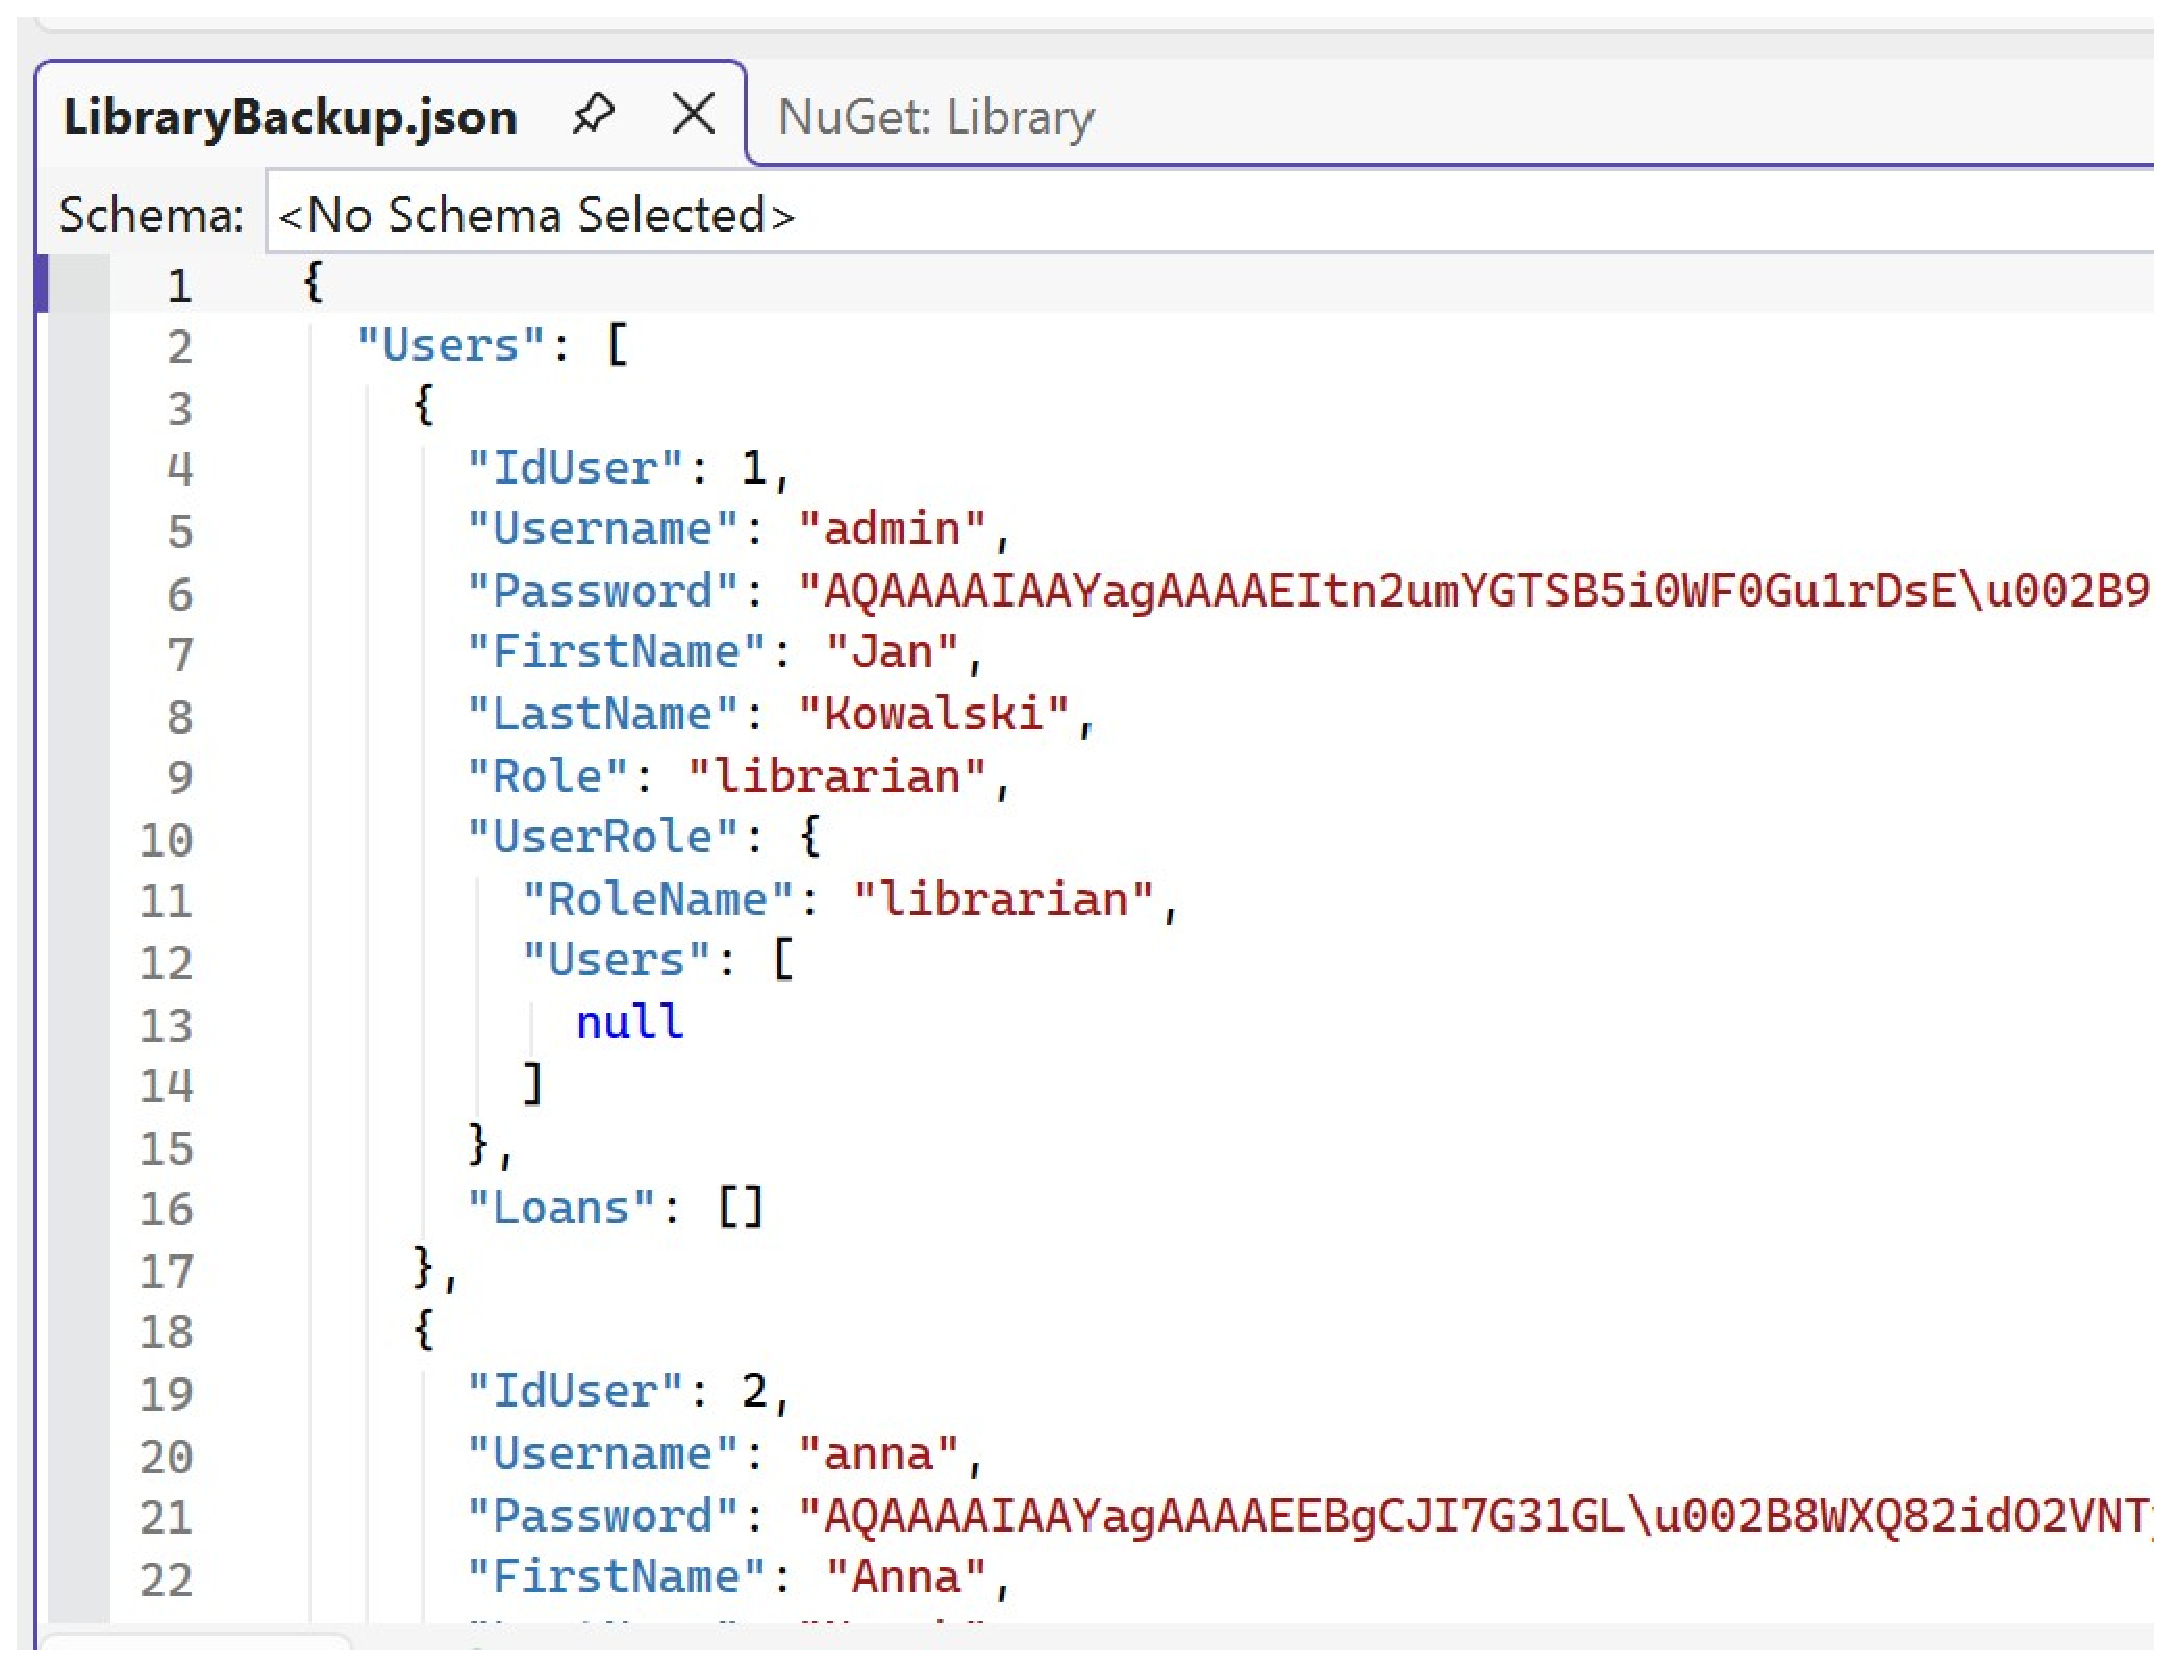
\includegraphics[width=0.9\linewidth]{figures/show/show15.eps}
    \caption{Przykładowa zawartość pliku eksportu danych \texttt{LibraryBackup.json}.\label{fig:ui_json_export}}
\end{figure}


\chapter{Podsumowanie}
Stworzony system pomyślnie zrealizował wszystkie kluczowe założenia projektowe. Aplikacja ułatwia codzienne procesy biblioteczne zarówno z perspektywy pracownika, jak i użytkownika. Napotkane wyzwania techniczne przy konfiguracji WPF zostały rozwiązane poprzez podział widoków. Potencjalnym kierunkiem na przyszły rozwój projektu jest zaimplementowanie rezerwacji książek przez użytkowników, wdrożenie autoryzacji biometrycznej czy utworzenie powiadomień e-mailowych z przypomnieniami o nadchodzących terminach zwrotu.